% !TEX program = xelatex
\documentclass[UTF8,fontset=fandol,a4paper,11pt]{ctexart}
\usepackage[margin=21mm,top=23mm,bottom=22mm,headheight=16pt]{geometry}
\usepackage{amsmath,amssymb,mathtools,bm}
\usepackage{tikz}
\usetikzlibrary{arrows.meta,calc,angles,quotes,patterns}
\usepackage{xcolor,booktabs,array,longtable,enumitem,fancyhdr,needspace}
\usepackage[unicode,hidelinks]{hyperref}
\definecolor{ink}{HTML}{24343C}
\definecolor{accent}{HTML}{166A70}
\definecolor{muted}{HTML}{65747A}
\definecolor{rulegray}{HTML}{D4DDE0}
\definecolor{warm}{HTML}{966037}
\color{ink}
\setlength{\parindent}{2em}
\setlength{\parskip}{4pt}
\linespread{1.12}
\AtBeginDocument{\setlength{\abovedisplayskip}{6pt plus 2pt minus 1pt}
\setlength{\belowdisplayskip}{6pt plus 2pt minus 1pt}
\setlength{\abovedisplayshortskip}{0pt plus 1pt}
\setlength{\belowdisplayshortskip}{4pt plus 1pt}}
\setlist[enumerate]{label=(\arabic*),leftmargin=2.3em,itemsep=3pt,topsep=4pt}
\setlist[itemize]{leftmargin=2em,itemsep=2pt,topsep=4pt}
\allowdisplaybreaks[1]
\setlength{\emergencystretch}{2em}
\setcounter{secnumdepth}{0}
\providecommand{\tightlist}{\setlength{\itemsep}{0pt}\setlength{\parskip}{0pt}}
\ctexset{section={format=\Large\bfseries\color{accent},beforeskip=10pt,afterskip=9pt},
subsection={format=\normalsize\bfseries\color{accent},beforeskip=10pt,afterskip=4pt},
subsubsection={format=\normalsize\bfseries,beforeskip=8pt,afterskip=3pt}}
\pagestyle{fancy}
\fancyhf{}
\fancyhead[L]{\small\color{muted}物理学难题集萃}
% 页眉仅保留书名；版本名称只在封面显示。
\fancyfoot[L]{\small\color{muted}\chapterlabel}
\fancyfoot[R]{\small\thepage}
\renewcommand{\headrulewidth}{0.4pt}
\renewcommand{\footrulewidth}{0pt}
\newcommand{\dd}{\mathop{}\!\mathrm{d}}
\newcommand{\vect}[1]{\bm{#1}}
\newcommand{\tagline}[1]{\noindent{\small\color{muted}#1}\par}
\newcommand{\result}[1]{\begin{equation*}\boxed{#1}\end{equation*}}
\newcommand{\figcaption}[1]{\par\vspace{2pt}{\small\color{muted}#1}\par}
\newcommand{\teach}[2]{\Needspace{4\baselineskip}\subsection*{讲解要点与追问}#1\par\smallskip\noindent\textbf{追问：}#2\par}
\newcommand{\workarea}{\par\vspace{7mm}\noindent{\small\color{muted}作答区}\par\vspace{4mm}
\noindent\textcolor{rulegray}{\rule{\linewidth}{0.3pt}}\par\vspace{16mm}
\noindent\textcolor{rulegray}{\rule{\linewidth}{0.3pt}}\par\vspace{16mm}
\noindent\textcolor{rulegray}{\rule{\linewidth}{0.3pt}}\par\vspace{16mm}
\noindent\textcolor{rulegray}{\rule{\linewidth}{0.3pt}}}
\tikzset{axis/.style={-{Stealth[length=2mm]},thin,color=muted},
motion/.style={-{Stealth[length=2.3mm]},thick,color=accent},
force/.style={-{Stealth[length=2.3mm]},thick,color=warm},
traj/.style={thick,color=accent},guide/.style={dashed,thin,color=muted},
object/.style={thick,color=ink},every node/.style={font=\small}}\widowpenalty=10000\clubpenalty=10000\displaywidowpenalty=10000\newcommand{\chapterlabel}{综合试题（三）}







\hypersetup{pdftitle={综合试题（三）·学生解答版},pdfauthor={}}

\begin{document}\pdfbookmark[0]{综合试题（三）}{cover}

\thispagestyle{empty}\vspace*{22mm}

\noindent{\Huge\bfseries 物理学难题集萃}\par\vspace{12mm}

\noindent{\LARGE 综合试题（三）}\par\vspace{12mm}

\noindent{\Large\color{accent}学生解答版}\par\vspace{9mm}

\noindent\textcolor{accent}{\rule{\linewidth}{1pt}}\par\vspace{9mm}

\noindent 第1--6题\par\vfill\clearpage

\pdfbookmark[1]{题目目录}{contents}\section*{题目目录}

\begin{longtable}{@{}r p{113mm} r@{}}\toprule 题号 & 题目 & 页码\\\midrule

\hyperref[q:1]{1} & \hyperref[q:1]{滚轮线的加速度、曲率与等时摆} & \pageref{q:1} \\

\hyperref[q:2]{2} & \hyperref[q:2]{限定地面投影范围的卫星轨道} & \pageref{q:2} \\

\hyperref[q:3]{3} & \hyperref[q:3]{悬挂弹性杆的长度与密度} & \pageref{q:3} \\

\hyperref[q:4]{4} & \hyperref[q:4]{阻尼振动、感应制动与受迫响应} & \pageref{q:4} \\

\hyperref[q:5]{5} & \hyperref[q:5]{随机选择、方向分布与二维分子速率} & \pageref{q:5} \\

\hyperref[q:6]{6} & \hyperref[q:6]{四相电源与断线后的浮动星点} & \pageref{q:6} \\

\bottomrule\end{longtable}

\clearpage

\pdfbookmark[2]{第 1 题 滚轮线的加速度、曲率与等时摆}{q1}

\section*{第 1 题\quad 滚轮线的加速度、曲率与等时摆}\label{q:1}


\begin{enumerate}
\item 半径$R$的圆环在水平地面向前纯滚动，环心速率恒为$v_0>0$。求环上任一点$P$在一周内加速度大小最大值与最小值之差。
\item 无论环心匀速还是变速前进，只要始终向前纯滚动，环上一点的轨迹都是同一条滚轮线。求轨迹最低接地点的曲率半径极限$\rho_1$及最高点的曲率半径$\rho_2$，并解释最低点为何需用极限表述。
\item 将生成圆环置于水平$x$轴下方沿轴纯滚动，得到向下凹的摆线轨道。小球从该轨道一拱内的任一光滑、非最低位置静止释放，无摩擦往返。已知其周期与质量及初位置无关，求全周期$T$，并由弧长坐标推导这种等时性。
\end{enumerate}
重力加速度为$g$；配图中区分向上滚轮线的接地尖点与下方凹轨道的光滑稳定最低点。


\begin{center}\begin{minipage}{.98\linewidth}\centering
\begin{tikzpicture}[scale=.85,transform shape]

\draw[axis] (-.4,0)--(5.7,0) node[right] {$x$};
\draw[object] (0,.8) circle (.8);
\fill (0,.8) circle (2pt) node[left] {$C$};
\draw[motion] (0,.8)--(1.2,.8) node[right] {$v_0$};
\fill (0,0) circle (2pt) node[below] {$P$};
\node at (2.6,2.3) {向上生成：接地处为尖点};
\draw[traj,domain=0:360,samples=160] plot ({.8*(rad(\x)-sin(\x))},{1*.8*(1-cos(\x))});
\begin{scope}[yshift=-2cm]
\draw[axis] (-.4,0)--(5.7,0);\draw[traj,domain=0:360,samples=160] plot ({.8*(rad(\x)-sin(\x))},{-1*.8*(1-cos(\x))});
\fill (2.513,-1.6) circle (2pt) node[below] {稳定最低点};
\node at (2.6,-2.4) {倒置凹轨道：最低点光滑};
\end{scope}

\end{tikzpicture}
\figcaption{图综三.1\quad 同一摆线的两种朝向；等时摆沿下方凹轨道运动。}
\end{minipage}\end{center}

\Needspace{6\baselineskip}\subsection*{解答}


图综三.1分别画圆环在地面上方滚动的轮上点轨迹，以及第（3）问在水平线下方生成的凹轨道。上方轨迹的最低位置是接地尖点；小球作等时摆动的最低位置则在下方轨道的光滑中部。

第（1）问，环心随地面作匀速直线运动，因此随环心平动的坐标系也是惯性系。$P$在此系中绕环心匀速转动，角速度$\omega=v_0/R$，加速度大小恒为
\[
|\boldsymbol a|=\omega^2R=\frac{v_0^2}{R}.
\]
匀速前进与无滑动接触使每转过$\mathrm d\theta$便平移$R\mathrm d\theta$，所以环心的恒定速率也固定了角速度。轮上点在环心系的运动半径始终为$R$，向心加速度模与转角无关，其方向随点的位置绕环心转动。在地面观察时还叠加恒定的平移速度，这会改变点的速率和速度方向，却不增加加速度。两个惯性系之间只差匀速平动，加速度矢量相同。故
\[
\boxed{a_{\max}-a_{\min}=0}.
\]
这里速度随位置变化，而指向环心的加速度保持相同的模，其方向随轮转动。
\begin{center}\begin{minipage}{.98\linewidth}\centering
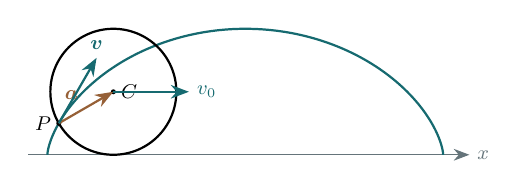
\begin{tikzpicture}[scale=.8,transform shape]
\draw[axis] (-.3,0)--(6.7,0) node[right] {$x$};\draw[traj] plot coordinates {(0.000000000,0.000000000) (0.000007088,0.000609173) (0.000056696,0.002435950) (0.000191292,0.005478105) (0.000453239,0.009731931) (0.000884748,0.015192247) (0.001527819,0.021852399) (0.002424200,0.029704274) (0.003615325,0.038738304) (0.005142271,0.048943484) (0.007045707,0.060307379) (0.009365842,0.072816145) (0.012142377,0.086454542) (0.015414459,0.101205954) (0.019220628,0.117052407) (0.023598776,0.133974596) (0.028586096,0.151951904) (0.034219042,0.170962427) (0.040533278,0.190983006) (0.047563640,0.211989246) (0.055344091,0.233955557) (0.063907679,0.256855175) (0.073286500,0.280660200) (0.083511656,0.305341630) (0.094613215,0.330869394) (0.106620183,0.357212390) (0.119560457,0.384338525) (0.133460802,0.412214748) (0.148346809,0.440807097) (0.164242870,0.470080736) (0.181172147,0.500000000) (0.199156543,0.530528437) (0.218216675,0.561628853) (0.238371849,0.593263357) (0.259640037,0.625393407) (0.282037856,0.657979857) (0.305580545,0.690983006) (0.330281951,0.724362644) (0.356154505,0.758078104) (0.383209216,0.792088309) (0.411455649,0.826351822) (0.440901918,0.860826899) (0.471554676,0.895471537) (0.503419106,0.930243526) (0.536498915,0.965100503) (0.570796327,1.000000000) (0.606312085,1.034899497) (0.643045447,1.069756474) (0.680994187,1.104528463) (0.720154598,1.139173101) (0.760521499,1.173648178) (0.802088236,1.207911691) (0.844846696,1.241921896) (0.888787311,1.275637356) (0.933899076,1.309016994) (0.980169556,1.342020143) (1.027584908,1.374606593) (1.076129890,1.406736643) (1.125787886,1.438371147) (1.176540924,1.469471563) (1.228369699,1.500000000) (1.281253591,1.529919264) (1.335170700,1.559192903) (1.390097863,1.587785252) (1.446010689,1.615661475) (1.502883584,1.642787610) (1.560689787,1.669130606) (1.619401397,1.694658370) (1.678989412,1.719339800) (1.739423761,1.743144825) (1.800673343,1.766044443) (1.862706063,1.788010754) (1.925488871,1.809016994) (1.988987804,1.829037573) (2.053168029,1.848048096) (2.117993878,1.866025404) (2.183428900,1.882947593) (2.249435901,1.898794046) (2.315976990,1.913545458) (2.383013625,1.927183855) (2.450506660,1.939692621) (2.518416394,1.951056516) (2.586702617,1.961261696) (2.655324663,1.970295726) (2.724241453,1.978147601) (2.793411551,1.984807753) (2.862793212,1.990268069) (2.932344435,1.994521895) (3.002023010,1.997564050) (3.071786572,1.999390827) (3.141592654,2.000000000) (3.211398735,1.999390827) (3.281162297,1.997564050) (3.350840872,1.994521895) (3.420392095,1.990268069) (3.489773756,1.984807753) (3.558943855,1.978147601) (3.627860644,1.970295726) (3.696482690,1.961261696) (3.764768913,1.951056516) (3.832678647,1.939692621) (3.900171682,1.927183855) (3.967208317,1.913545458) (4.033749406,1.898794046) (4.099756407,1.882947593) (4.165191429,1.866025404) (4.230017278,1.848048096) (4.294197503,1.829037573) (4.357696437,1.809016994) (4.420479245,1.788010754) (4.482511964,1.766044443) (4.543761546,1.743144825) (4.604195895,1.719339800) (4.663783910,1.694658370) (4.722495520,1.669130606) (4.780301723,1.642787610) (4.837174618,1.615661475) (4.893087444,1.587785252) (4.948014607,1.559192903) (5.001931716,1.529919264) (5.054815609,1.500000000) (5.106644383,1.469471563) (5.157397421,1.438371147) (5.207055418,1.406736643) (5.255600400,1.374606593) (5.303015751,1.342020143) (5.349286231,1.309016994) (5.394397996,1.275637356) (5.438338611,1.241921896) (5.481097071,1.207911691) (5.522663808,1.173648178) (5.563030709,1.139173101) (5.602191121,1.104528463) (5.640139861,1.069756474) (5.676873222,1.034899497) (5.712388980,1.000000000) (5.746686392,0.965100503) (5.779766201,0.930243526) (5.811630631,0.895471537) (5.842283389,0.860826899) (5.871729659,0.826351822) (5.899976091,0.792088309) (5.927030802,0.758078104) (5.952903357,0.724362644) (5.977604762,0.690983006) (6.001147452,0.657979857) (6.023545270,0.625393407) (6.044813459,0.593263357) (6.064968632,0.561628853) (6.084028764,0.530528437) (6.102013160,0.500000000) (6.118942437,0.470080736) (6.134838499,0.440807097) (6.149724505,0.412214748) (6.163624850,0.384338525) (6.176565124,0.357212390) (6.188572092,0.330869394) (6.199673652,0.305341630) (6.209898807,0.280660200) (6.219277628,0.256855175) (6.227841216,0.233955557) (6.235621667,0.211989246) (6.242652029,0.190983006) (6.248966265,0.170962427) (6.254599211,0.151951904) (6.259586532,0.133974596) (6.263964679,0.117052407) (6.267770848,0.101205954) (6.271042930,0.086454542) (6.273819465,0.072816145) (6.276139600,0.060307379) (6.278043036,0.048943484) (6.279569983,0.038738304) (6.280761108,0.029704274) (6.281657488,0.021852399) (6.282300560,0.015192247) (6.282732068,0.009731931) (6.282994015,0.005478105) (6.283128611,0.002435950) (6.283178219,0.000609173) (6.283185307,0.000000000)};\draw[thick] (1.0471975511965976,1) circle(1);\fill (1.0471975511965976,1) circle(.04) node[right] {$C$};\fill (0.18117214741215903,0.4999999999999999) circle(.04) node[left] {$P$};\draw[force] (0.18117214741215903,0.4999999999999999)--(1.0471975511965976,1) node[midway,above left] {$\boldsymbol a$};\draw[motion] (0.18117214741215903,0.4999999999999999)--(0.781172147412159,1.539230484541326) node[above] {$\boldsymbol v$};\draw[motion] (1.0471975511965976,1)--(2.2471975511965976,1) node[right] {$v_0$};
\end{tikzpicture}
\figcaption{解图综三.1A\quad 真实滚轮线与生成圆，横纵同尺度；加速度指向轮心}
\end{minipage}\end{center}
第（2）问，解图综三.1A取地面接地点为参数起点，$y$向上。设圆环转过$\theta$，纯滚动给环心平移$R\theta$，故
\[
x=R(\theta-\sin\theta),\qquad
y=R(1-\cos\theta).
\]
环心坐标为$(R\theta,R)$，轮上点相对环心的坐标为$(-R\sin\theta,-R\cos\theta)$，逐分量相加就是这组参数式。只要向前纯滚动，转角可以随时间非匀速增加，所有位置仍依次落在这条曲线上。轨迹的几何形状与$\theta$随时间变化的方式无关。为计算曲率，可选择环心匀速的方便运动：
\[
\begin{aligned}
\dot x&=v_0(1-\cos\theta),&
\dot y&=v_0\sin\theta,\\
\ddot x&=\frac{v_0^2}{R}\sin\theta,&
\ddot y&=\frac{v_0^2}{R}\cos\theta.
\end{aligned}
\]
对$0<\theta<2\pi$，
\[
v=2v_0\sin\frac\theta2,\qquad
|\dot x\ddot y-\dot y\ddot x|
=\frac{2v_0^3}{R}\sin^2\frac\theta2.
\]
速度平方化简用$(1-\cos\theta)^2+\sin^2\theta=2(1-\cos\theta)=4\sin^2(\theta/2)$。叉积中的三角项为$(1-\cos\theta)\cos\theta-\sin^2\theta=\cos\theta-1$，取绝对值得到上式。曲率只由轨迹的局部几何决定，分子、分母中所选生成速率的三次因子随后相消。因此正则点曲率半径为
\[
\boxed{\rho=
\frac{(\dot x^2+\dot y^2)^{3/2}}
{|\dot x\ddot y-\dot y\ddot x|}
=4R\sin\frac\theta2}.
\]
\begin{center}\begin{minipage}{.98\linewidth}\centering
\begin{tikzpicture}[scale=.8,transform shape]
\draw[axis] (-1,0)--(1.2,0) node[right] {$x$};\draw[axis] (0,0)--(0,3.1) node[above] {切线极限};\draw[traj] plot coordinates {(-0.661151273,2.426346325) (-0.637173821,2.369237475) (-0.613764646,2.312691696) (-0.590918091,2.256714643) (-0.568628439,2.201311914) (-0.546889920,2.146489049) (-0.525696707,2.092251530) (-0.505042920,2.038604781) (-0.484922624,1.985554167) (-0.465329832,1.933104992) (-0.446258502,1.881262502) (-0.427702542,1.830031880) (-0.409655808,1.779418250) (-0.392112104,1.729426673) (-0.375065184,1.680062148) (-0.358508754,1.631329612) (-0.342436469,1.583233937) (-0.326841936,1.535779934) (-0.311718716,1.488972347) (-0.297060319,1.442815857) (-0.282860213,1.397315081) (-0.269111817,1.352474567) (-0.255808506,1.308298801) (-0.242943610,1.264792199) (-0.230510417,1.221959112) (-0.218502169,1.179803824) (-0.206912067,1.138330549) (-0.195733270,1.097543436) (-0.184958897,1.057446563) (-0.174582025,1.018043939) (-0.164595691,0.979339505) (-0.154992895,0.941337131) (-0.145766596,0.904040618) (-0.136909717,0.867453694) (-0.128415144,0.831580020) (-0.120275727,0.796423181) (-0.112484279,0.761986694) (-0.105033581,0.728274003) (-0.097916376,0.695288478) (-0.091125376,0.663033417) (-0.084653262,0.631512048) (-0.078492679,0.600727521) (-0.072636245,0.570682915) (-0.067076544,0.541381235) (-0.061806134,0.512825411) (-0.056817540,0.485018297) (-0.052103263,0.457962676) (-0.047655773,0.431661252) (-0.043467515,0.406116655) (-0.039530908,0.381331441) (-0.035838347,0.357308087) (-0.032382199,0.334048996) (-0.029154811,0.311556494) (-0.026148506,0.289832829) (-0.023355585,0.268880175) (-0.020768326,0.248700626) (-0.018378989,0.229296201) (-0.016179812,0.210668840) (-0.014163015,0.192820405) (-0.012320801,0.175752682) (-0.010645354,0.159467377) (-0.009128840,0.143966119) (-0.007763413,0.129250458) (-0.006541207,0.115321865) (-0.005454347,0.102181733) (-0.004494940,0.089831377) (-0.003655083,0.078272030) (-0.002926859,0.067504850) (-0.002302342,0.057530913) (-0.001773593,0.048351216) (-0.001332667,0.039966678) (-0.000971606,0.032378136) (-0.000682448,0.025586350) (-0.000457221,0.019591998) (-0.000287948,0.014395681) (-0.000166646,0.009997917) (-0.000085327,0.006399147) (-0.000035998,0.003599730) (-0.000010666,0.001599947) (-0.000001333,0.000399997) (0.000000000,0.000000000) (0.000001333,0.000399997) (0.000010666,0.001599947) (0.000035998,0.003599730) (0.000085327,0.006399147) (0.000166646,0.009997917) (0.000287948,0.014395681) (0.000457221,0.019591998) (0.000682448,0.025586350) (0.000971606,0.032378136) (0.001332667,0.039966678) (0.001773593,0.048351216) (0.002302342,0.057530913) (0.002926859,0.067504850) (0.003655083,0.078272030) (0.004494940,0.089831377) (0.005454347,0.102181733) (0.006541207,0.115321865) (0.007763413,0.129250458) (0.009128840,0.143966119) (0.010645354,0.159467377) (0.012320801,0.175752682) (0.014163015,0.192820405) (0.016179812,0.210668840) (0.018378989,0.229296201) (0.020768326,0.248700626) (0.023355585,0.268880175) (0.026148506,0.289832829) (0.029154811,0.311556494) (0.032382199,0.334048996) (0.035838347,0.357308087) (0.039530908,0.381331441) (0.043467515,0.406116655) (0.047655773,0.431661252) (0.052103263,0.457962676) (0.056817540,0.485018297) (0.061806134,0.512825411) (0.067076544,0.541381235) (0.072636245,0.570682915) (0.078492679,0.600727521) (0.084653262,0.631512048) (0.091125376,0.663033417) (0.097916376,0.695288478) (0.105033581,0.728274003) (0.112484279,0.761986694) (0.120275727,0.796423181) (0.128415144,0.831580020) (0.136909717,0.867453694) (0.145766596,0.904040618) (0.154992895,0.941337131) (0.164595691,0.979339505) (0.174582025,1.018043939) (0.184958897,1.057446563) (0.195733270,1.097543436) (0.206912067,1.138330549) (0.218502169,1.179803824) (0.230510417,1.221959112) (0.242943610,1.264792199) (0.255808506,1.308298801) (0.269111817,1.352474567) (0.282860213,1.397315081) (0.297060319,1.442815857) (0.311718716,1.488972347) (0.326841936,1.535779934) (0.342436469,1.583233937) (0.358508754,1.631329612) (0.375065184,1.680062148) (0.392112104,1.729426673) (0.409655808,1.779418250) (0.427702542,1.830031880) (0.446258502,1.881262502) (0.465329832,1.933104992) (0.484922624,1.985554167) (0.505042920,2.038604781) (0.525696707,2.092251530) (0.546889920,2.146489049) (0.568628439,2.201311914) (0.590918091,2.256714643) (0.613764646,2.312691696) (0.637173821,2.369237475) (0.661151273,2.426346325)};\fill (0,0) circle(.04) node[below] {接地尖点};\node at (0,-.8) {$x\sim R\theta^3/6,\quad y\sim R\theta^2/2$};
\end{tikzpicture}
\figcaption{解图综三.1B\quad 真实尖点曲线，两坐标共同放大8倍}
\end{minipage}\end{center}
解图综三.1B放大最低接地位置。$\theta=0$时轨迹参数导数为零，是尖点，不是普通光滑点；曲率由两侧邻近的正则点取极限描述。邻近点满足
\[
x\simeq\frac R6\theta^3,\qquad
y\simeq\frac R2\theta^2,
\]
两侧切线都趋于竖直方向。更具体地，$\mathrm dx/\mathrm dy=(1-\cos\theta)/\sin\theta=\tan(\theta/2)\to0$，横向变化相对竖向变化更小。速度在尖点为零，切线却由邻近位移方向确定，图B的两侧分支都贴向同一竖直直线。由上面的正则点公式，
\[
\boxed{\rho_1=\lim_{\theta\to0^+}\rho=0}.
\]
曲率半径趋零描述的是邻近正则曲线的弯曲圆越来越小。与此同时，速度也趋零，比较二者的相对阶数才给法向加速度；这两个极限与尖点处的有限总加速度分别对应不同量。在所选匀速生成运动中，法向加速度为
$a_n=(v_0^2/R)\sin(\theta/2)$，也趋于零；尖点处有限的总加速度主要沿切线极限方向，切向与法向分量分别按速度方向分解。

最高点$\theta=\pi$是光滑点，速度水平、大小$2v_0$，加速度竖直向下，纯法向，故
\[
\boxed{\rho_2=\frac{(2v_0)^2}{v_0^2/R}=4R}.
\]
它与参数曲率式在$\theta=\pi$的值一致。
\begin{center}\begin{minipage}{.98\linewidth}\centering
\begin{tikzpicture}[scale=.8,transform shape]
\draw[axis] (-.3,0)--(6.7,0) node[right] {$x$};\draw[axis] (0,.4)--(0,-2.7) node[below] {$y$向下};\draw[traj] plot coordinates {(0.000000000,-0.000000000) (0.000007088,-0.000609173) (0.000056696,-0.002435950) (0.000191292,-0.005478105) (0.000453239,-0.009731931) (0.000884748,-0.015192247) (0.001527819,-0.021852399) (0.002424200,-0.029704274) (0.003615325,-0.038738304) (0.005142271,-0.048943484) (0.007045707,-0.060307379) (0.009365842,-0.072816145) (0.012142377,-0.086454542) (0.015414459,-0.101205954) (0.019220628,-0.117052407) (0.023598776,-0.133974596) (0.028586096,-0.151951904) (0.034219042,-0.170962427) (0.040533278,-0.190983006) (0.047563640,-0.211989246) (0.055344091,-0.233955557) (0.063907679,-0.256855175) (0.073286500,-0.280660200) (0.083511656,-0.305341630) (0.094613215,-0.330869394) (0.106620183,-0.357212390) (0.119560457,-0.384338525) (0.133460802,-0.412214748) (0.148346809,-0.440807097) (0.164242870,-0.470080736) (0.181172147,-0.500000000) (0.199156543,-0.530528437) (0.218216675,-0.561628853) (0.238371849,-0.593263357) (0.259640037,-0.625393407) (0.282037856,-0.657979857) (0.305580545,-0.690983006) (0.330281951,-0.724362644) (0.356154505,-0.758078104) (0.383209216,-0.792088309) (0.411455649,-0.826351822) (0.440901918,-0.860826899) (0.471554676,-0.895471537) (0.503419106,-0.930243526) (0.536498915,-0.965100503) (0.570796327,-1.000000000) (0.606312085,-1.034899497) (0.643045447,-1.069756474) (0.680994187,-1.104528463) (0.720154598,-1.139173101) (0.760521499,-1.173648178) (0.802088236,-1.207911691) (0.844846696,-1.241921896) (0.888787311,-1.275637356) (0.933899076,-1.309016994) (0.980169556,-1.342020143) (1.027584908,-1.374606593) (1.076129890,-1.406736643) (1.125787886,-1.438371147) (1.176540924,-1.469471563) (1.228369699,-1.500000000) (1.281253591,-1.529919264) (1.335170700,-1.559192903) (1.390097863,-1.587785252) (1.446010689,-1.615661475) (1.502883584,-1.642787610) (1.560689787,-1.669130606) (1.619401397,-1.694658370) (1.678989412,-1.719339800) (1.739423761,-1.743144825) (1.800673343,-1.766044443) (1.862706063,-1.788010754) (1.925488871,-1.809016994) (1.988987804,-1.829037573) (2.053168029,-1.848048096) (2.117993878,-1.866025404) (2.183428900,-1.882947593) (2.249435901,-1.898794046) (2.315976990,-1.913545458) (2.383013625,-1.927183855) (2.450506660,-1.939692621) (2.518416394,-1.951056516) (2.586702617,-1.961261696) (2.655324663,-1.970295726) (2.724241453,-1.978147601) (2.793411551,-1.984807753) (2.862793212,-1.990268069) (2.932344435,-1.994521895) (3.002023010,-1.997564050) (3.071786572,-1.999390827) (3.141592654,-2.000000000) (3.211398735,-1.999390827) (3.281162297,-1.997564050) (3.350840872,-1.994521895) (3.420392095,-1.990268069) (3.489773756,-1.984807753) (3.558943855,-1.978147601) (3.627860644,-1.970295726) (3.696482690,-1.961261696) (3.764768913,-1.951056516) (3.832678647,-1.939692621) (3.900171682,-1.927183855) (3.967208317,-1.913545458) (4.033749406,-1.898794046) (4.099756407,-1.882947593) (4.165191429,-1.866025404) (4.230017278,-1.848048096) (4.294197503,-1.829037573) (4.357696437,-1.809016994) (4.420479245,-1.788010754) (4.482511964,-1.766044443) (4.543761546,-1.743144825) (4.604195895,-1.719339800) (4.663783910,-1.694658370) (4.722495520,-1.669130606) (4.780301723,-1.642787610) (4.837174618,-1.615661475) (4.893087444,-1.587785252) (4.948014607,-1.559192903) (5.001931716,-1.529919264) (5.054815609,-1.500000000) (5.106644383,-1.469471563) (5.157397421,-1.438371147) (5.207055418,-1.406736643) (5.255600400,-1.374606593) (5.303015751,-1.342020143) (5.349286231,-1.309016994) (5.394397996,-1.275637356) (5.438338611,-1.241921896) (5.481097071,-1.207911691) (5.522663808,-1.173648178) (5.563030709,-1.139173101) (5.602191121,-1.104528463) (5.640139861,-1.069756474) (5.676873222,-1.034899497) (5.712388980,-1.000000000) (5.746686392,-0.965100503) (5.779766201,-0.930243526) (5.811630631,-0.895471537) (5.842283389,-0.860826899) (5.871729659,-0.826351822) (5.899976091,-0.792088309) (5.927030802,-0.758078104) (5.952903357,-0.724362644) (5.977604762,-0.690983006) (6.001147452,-0.657979857) (6.023545270,-0.625393407) (6.044813459,-0.593263357) (6.064968632,-0.561628853) (6.084028764,-0.530528437) (6.102013160,-0.500000000) (6.118942437,-0.470080736) (6.134838499,-0.440807097) (6.149724505,-0.412214748) (6.163624850,-0.384338525) (6.176565124,-0.357212390) (6.188572092,-0.330869394) (6.199673652,-0.305341630) (6.209898807,-0.280660200) (6.219277628,-0.256855175) (6.227841216,-0.233955557) (6.235621667,-0.211989246) (6.242652029,-0.190983006) (6.248966265,-0.170962427) (6.254599211,-0.151951904) (6.259586532,-0.133974596) (6.263964679,-0.117052407) (6.267770848,-0.101205954) (6.271042930,-0.086454542) (6.273819465,-0.072816145) (6.276139600,-0.060307379) (6.278043036,-0.048943484) (6.279569983,-0.038738304) (6.280761108,-0.029704274) (6.281657488,-0.021852399) (6.282300560,-0.015192247) (6.282732068,-0.009731931) (6.282994015,-0.005478105) (6.283128611,-0.002435950) (6.283178219,-0.000609173) (6.283185307,-0.000000000)};\fill (3.141592653589793,-2) circle(.05) node[below] {稳定最低点};\fill (3.141592653589793,2) circle(.05) node[above] {$O$};\draw[guide] (3.141592653589793,-2)--(3.141592653589793,2) node[midway,right] {$4R$};\draw[dashed,color=warm] plot coordinates {(1.583919284,-1.684243976) (1.633179540,-1.704684855) (1.682707953,-1.724467134) (1.732495720,-1.743587295) (1.782533990,-1.762041939) (1.832813866,-1.779827785) (1.883326411,-1.796941672) (1.934062644,-1.813380558) (1.985013546,-1.829141518) (2.036170059,-1.844221753) (2.087523089,-1.858618581) (2.139063506,-1.872329442) (2.190782148,-1.885351899) (2.242669820,-1.897683638) (2.294717299,-1.909322465) (2.346915330,-1.920266311) (2.399254636,-1.930513232) (2.451725911,-1.940061405) (2.504319827,-1.948909134) (2.557027034,-1.957054844) (2.609838163,-1.964497088) (2.662743824,-1.971234543) (2.715734613,-1.977266012) (2.768801109,-1.982590421) (2.821933878,-1.987206825) (2.875123474,-1.991114403) (2.928360442,-1.994312459) (2.981635317,-1.996800427) (3.034938628,-1.998577862) (3.088260900,-1.999644450) (3.141592654,-2.000000000) (3.194924407,-1.999644450) (3.248246679,-1.998577862) (3.301549990,-1.996800427) (3.354824866,-1.994312459) (3.408061833,-1.991114403) (3.461251429,-1.987206825) (3.514384198,-1.982590421) (3.567450694,-1.977266012) (3.620441483,-1.971234543) (3.673347144,-1.964497088) (3.726158273,-1.957054844) (3.778865480,-1.948909134) (3.831459396,-1.940061405) (3.883930671,-1.930513232) (3.936269977,-1.920266311) (3.988468009,-1.909322465) (4.040515487,-1.897683638) (4.092403159,-1.885351899) (4.144121801,-1.872329442) (4.195662218,-1.858618581) (4.247015248,-1.844221753) (4.298171761,-1.829141518) (4.349122663,-1.813380558) (4.399858896,-1.796941672) (4.450371441,-1.779827785) (4.500651317,-1.762041939) (4.550689587,-1.743587295) (4.600477354,-1.724467134) (4.650005767,-1.704684855) (4.699266023,-1.684243976)};
\end{tikzpicture}
\figcaption{解图综三.1C\quad 倒置凹轨道最低点的曲率圆半径4R，横纵同尺度}
\end{minipage}\end{center}
第（3）问，解图综三.1C改取$y$向下，凹轨道仍可用
$x=R(\theta-\sin\theta),y=R(1-\cos\theta)$表示。稳定最低点在$\theta=\pi$，其曲率半径是$4R$，它位于一拱的光滑中部。

两种朝向的最高、最低位置随倒置互换，第三问用的光滑最低点对应第二问的光滑最高点，几何曲率半径保持相同。取该点附近的短轨道，用其曲率圆近似时，误差从更高阶位移开始，线性的切向恢复力由这个半径决定。

因为已知周期与振幅无关，可以取任意小振幅。在最低点附近，轨道等同于半径$4R$的曲率圆，等效小角单摆长$4R$：
\[
\boxed{T=2\pi\sqrt{\frac{4R}{g}}
=4\pi\sqrt{\frac Rg}}.
\]
这个推理用到了题给等时性；对一般光滑曲线，用最低点曲率只能求小振幅周期，有限振幅还由轨道整段的势能关系决定。
\begin{center}\begin{minipage}{.98\linewidth}\centering
\begin{tikzpicture}[scale=.8,transform shape]
\draw[axis] (0,0)--(10.7,0) node[right] {$s/R$};
\draw[axis] (0,0)--(0,3.2) node[above] {$\Delta h/R$};\foreach \y/\lab in {0/0,1.3/1,2.6/2}{\draw[thin] (0,\y)--(-.08,\y) node[left] {$\lab$};}
\node[above] at (5,3.5) {有向弧长坐标下，高度精确为二次函数};
\draw[traj] plot coordinates {(0.250000000,2.346500000) (0.329166667,2.268935139) (0.408333333,2.192673889) (0.487500000,2.117716250) (0.566666667,2.044062222) (0.645833333,1.971711806) (0.725000000,1.900665000) (0.804166667,1.830921806) (0.883333333,1.762482222) (0.962500000,1.695346250) (1.041666667,1.629513889) (1.120833333,1.564985139) (1.200000000,1.501760000) (1.279166667,1.439838472) (1.358333333,1.379220556) (1.437500000,1.319906250) (1.516666667,1.261895556) (1.595833333,1.205188472) (1.675000000,1.149785000) (1.754166667,1.095685139) (1.833333333,1.042888889) (1.912500000,0.991396250) (1.991666667,0.941207222) (2.070833333,0.892321806) (2.150000000,0.844740000) (2.229166667,0.798461806) (2.308333333,0.753487222) (2.387500000,0.709816250) (2.466666667,0.667448889) (2.545833333,0.626385139) (2.625000000,0.586625000) (2.704166667,0.548168472) (2.783333333,0.511015556) (2.862500000,0.475166250) (2.941666667,0.440620556) (3.020833333,0.407378472) (3.100000000,0.375440000) (3.179166667,0.344805139) (3.258333333,0.315473889) (3.337500000,0.287446250) (3.416666667,0.260722222) (3.495833333,0.235301806) (3.575000000,0.211185000) (3.654166667,0.188371806) (3.733333333,0.166862222) (3.812500000,0.146656250) (3.891666667,0.127753889) (3.970833333,0.110155139) (4.050000000,0.093860000) (4.129166667,0.078868472) (4.208333333,0.065180556) (4.287500000,0.052796250) (4.366666667,0.041715556) (4.445833333,0.031938472) (4.525000000,0.023465000) (4.604166667,0.016295139) (4.683333333,0.010428889) (4.762500000,0.005866250) (4.841666667,0.002607222) (4.920833333,0.000651806) (5.000000000,0.000000000) (5.079166667,0.000651806) (5.158333333,0.002607222) (5.237500000,0.005866250) (5.316666667,0.010428889) (5.395833333,0.016295139) (5.475000000,0.023465000) (5.554166667,0.031938472) (5.633333333,0.041715556) (5.712500000,0.052796250) (5.791666667,0.065180556) (5.870833333,0.078868472) (5.950000000,0.093860000) (6.029166667,0.110155139) (6.108333333,0.127753889) (6.187500000,0.146656250) (6.266666667,0.166862222) (6.345833333,0.188371806) (6.425000000,0.211185000) (6.504166667,0.235301806) (6.583333333,0.260722222) (6.662500000,0.287446250) (6.741666667,0.315473889) (6.820833333,0.344805139) (6.900000000,0.375440000) (6.979166667,0.407378472) (7.058333333,0.440620556) (7.137500000,0.475166250) (7.216666667,0.511015556) (7.295833333,0.548168472) (7.375000000,0.586625000) (7.454166667,0.626385139) (7.533333333,0.667448889) (7.612500000,0.709816250) (7.691666667,0.753487222) (7.770833333,0.798461806) (7.850000000,0.844740000) (7.929166667,0.892321806) (8.008333333,0.941207222) (8.087500000,0.991396250) (8.166666667,1.042888889) (8.245833333,1.095685139) (8.325000000,1.149785000) (8.404166667,1.205188472) (8.483333333,1.261895556) (8.562500000,1.319906250) (8.641666667,1.379220556) (8.720833333,1.439838472) (8.800000000,1.501760000) (8.879166667,1.564985139) (8.958333333,1.629513889) (9.037500000,1.695346250) (9.116666667,1.762482222) (9.195833333,1.830921806) (9.275000000,1.900665000) (9.354166667,1.971711806) (9.433333333,2.044062222) (9.512500000,2.117716250) (9.591666667,2.192673889) (9.670833333,2.268935139) (9.750000000,2.346500000)};
\node[below] at (0,-.12) {$-4$};
\node[below] at (5,-.12) {$0$};
\node[below] at (10,-.12) {$4$};
\end{tikzpicture}
\figcaption{解图综三.1D\quad 有向弧长坐标下，高度精确为二次函数}
\end{minipage}\end{center}
解图综三.1D把最低点量起的有向弧长$s$与竖直上升高度相联系。沿一拱$0<\theta<2\pi$，
\[
\frac{ds}{d\theta}=2R\sin\frac\theta2,\qquad
s(\pi)=0,
\]
积分下限选在$\theta=\pi$，有$s=\int_\pi^\theta2R\sin(\eta/2)\mathrm d\eta=-4R\cos(\theta/2)$，使右侧位置为正、左侧位置为负。这个符号约定和$\mathrm ds/\mathrm d\theta>0$一致，所以
\[
s=-4R\cos\frac\theta2.
\]
小球相对最低点的竖直上升高度为
\[
\Delta h=2R-y=2R\cos^2\frac\theta2
=\frac{s^2}{8R}.
\]
以弧长作广义坐标，沿轨道的速率就是$|\dot s|$，动能为$m\dot s^2/2$，势能为$mg\Delta h$。沿弧长的重力分量为势能的负导数，质量在运动方程两端相消，切向运动方程或能量的弧长导数给
\[
m\ddot s=-mg\frac{d\Delta h}{ds}
=-\frac{mg}{4R}s,
\qquad
\ddot s+\frac g{4R}s=0.
\]
它对一拱内的有限振幅也是严格简谐方程，再次给全周期$4\pi\sqrt{R/g}$。一侧释放至最低点为四分之一周期，完整往返包含四段这样的运动。
从静止释放时$s(0)=s_0,\dot s(0)=0$，因此$s=s_0\cos[\sqrt{g/(4R)}\,t]$；质量和$s_0$只影响能量及运动幅度，方程中的频率保持相同。振幅限定在$|s_0|<4R$，对应一拱内的光滑释放点，运动在两个等高转向点之间往返。到最低点时速度最大，再爬升到另一侧转向，接着按相反次序返回，完整过程构成上式的一个周期。



\Needspace{13\baselineskip}

\pdfbookmark[2]{第 2 题 限定地面投影范围的卫星轨道}{q2}

\section*{第 2 题\quad 限定地面投影范围的卫星轨道}\label{q:2}


在一个假想规则下，卫星与地心连线同地表的交点必须始终位于本国领土或领海。忽略摄动，地球视为球形。取地球自转周期$T_0=1\,\mathrm d=86400\,\mathrm s$，同步圆轨道的地心距离$R_0=4.21\times10^4\,\mathrm{km}$。
\begin{enumerate}
\item 一个国家仅有北纬$20^\circ$至$50^\circ$的领土，能否发射入轨后不靠动力且始终不越界的卫星？另一个国家有北纬$15^\circ$至南纬$10^\circ$的领土，且有赤道领土，能否找到一种可行轨道？
\item 某国在赤道只拥有总经度宽$\theta_0=2^\circ$的连续区域，发射周期$T_0$的赤道面无动力椭圆轨道卫星。长短半轴为$A,B$，焦距$C=\sqrt{A^2-B^2}$，偏心率$e=C/A\ll1$。求使卫星地面投影不越出该经度范围的最大$e$，保留一阶推导，并说明全摆幅与半摆幅。
\item 另有卫星需靠动力定点在北纬$\phi=40^\circ$的某城市上空，距地心恰为$R_0$。入轨后卫星主体质量100公斤，火箭空载1000公斤，燃料9000公斤；喷气相对速度$u=5\,\mathrm{km/s}$。求维持该位置的最久时间，给出所需推力方向和随质量变化的燃耗关系。
\end{enumerate}
第（2）问可选择初始经度使投影摆动区间居中；第（3）问假定推力连续可调，忽略其他燃耗。


\begin{center}\begin{minipage}{.98\linewidth}\centering
\begin{tikzpicture}[scale=.8,transform shape]

\draw[object] (0,0) circle (1.7);
\draw[guide] (-2,0)--(2,0) node[right] {赤道};
\draw[guide] (0,-2.1)--(0,2.1) node[above] {地轴};
\draw[traj] (-1.597477455,0.581434244)--(1.597477455,0.581434244);
\draw[traj] (-1.092738936,1.302275553)--(1.092738936,1.302275553);
\node[right] at (1.7,1) {$20^\circ$至$50^\circ$};
\begin{scope}[xshift=6.5cm]
\draw[object] (0,0) circle (1.1);
\draw[guide] (0,-1.7)--(0,2.3) node[above] {$z$};
\draw[guide] (-1.5,0)--(2.8,0);
\fill (2.1,1.76) circle (3pt) node[above right] {动力定点};
\draw[object] (0,0)--(2.1,1.76) node[midway,above left] {$R_0$};
\draw[guide] (.8,0) arc[start angle=0,end angle=40,radius=.8];
\node at (1.05,.35) {$\phi$};
\end{scope}

\end{tikzpicture}
\figcaption{图综三.2\quad 不含赤道的纬带与固定北纬位置；距离均由地心量起。}
\end{minipage}\end{center}

\Needspace{6\baselineskip}\subsection*{解答}


图综三.2先区别不含赤道的纬带、赤道椭圆的经度摆动，以及定纬动力飞行。以下按题给的投影范围判断轨道。

第（1）问，无动力平方反比引力轨道所在平面通过地心。非赤道轨道平面与赤道平面相交，卫星每周必经过赤道；若轨道恰为赤道面，其地面纬度始终为零。两种情况都不可能始终留在北纬$20^\circ$至$50^\circ$，故第一个国家不可行。

第二个国家拥有赤道领土，可在本国赤道某经度上方放置顺行同步圆轨道卫星，其地面投影固定于该点。这一轨道给出了符合要求的无动力可行例子。
\begin{center}\begin{minipage}{.98\linewidth}\centering
\begin{tikzpicture}[scale=.8,transform shape]
\draw[object] (0,0) ellipse (3.0 and 2.749545416973504);\fill (0,0) circle(.04) node[below left] {$O$};\fill (1.2000000000000002,0) circle(.04) node[below right] {$E$};\fill (0.3198902119638038,2.7338696040454074) circle(.04) node[above] {$P$};\fill (0.3198902119638038,-2.7338696040454074) circle(.04) node[below] {$P'$};\draw[guide] (1.2000000000000002,0)--(0.3198902119638038,2.7338696040454074);\draw[guide] (1.2000000000000002,0)--(0.3198902119638038,-2.7338696040454074);\draw[guide] (0.3198902119638038,-2.7338696040454074)--(0.3198902119638038,2.7338696040454074);\draw[axis] (-3.5,0)--(3.6,0) node[right] {$x$};\node at (0,3.6) {$P,P':\ \omega=\omega_0,\quad r_*^2=AB$};\node at (0,-3.6) {几何图放大偏心率，折返点按精确角速度条件定位};
\end{tikzpicture}
\figcaption{解图综三.2A\quad 地心位于焦点，折返点位置由面积速度与同步角速度共同给出}
\end{minipage}\end{center}
顺行同步圆轨道的周期等于地球自转周期，轨道平面与赤道重合，所以卫星和该国赤道上的参考点保持相同角速度，地心连线的表面交点便固定。这是存在性判断，采用圆轨道即可满足本问。

第（2）问，解图综三.2A把地心$E$置于椭圆右焦点，椭圆中心为坐标原点，$E=(C,0)$。地球角速度$\omega_0=2\pi/T_0$。以$K$记卫星绕地心的面积速度，
\[
K=\frac12r^2\omega,\qquad
T_0=\frac{\pi AB}{K}.
\]
地固经度相对惯性方向减去地球转角，其变化率为$\dot\lambda=\omega-\omega_0$。一周后两者都转过$2\pi$，累计相对经度回到起点；在中间各段，其变化率仍可正或负，所以出现往返。

卫星角速度有快于和慢于$\omega_0$的部分，投影相对地面的经度先向一侧移动再折返。设两折返点为$P,P'$，在它们处$\omega=\omega_0$，对应地心距离$r_*$满足
\[
K=\frac12r_*^2\omega_0
=\frac{\pi AB}{T_0}
\ \Longrightarrow\
\boxed{r_*^2=AB}.
\]
快行段位于近地点一侧，地固投影向东；慢行段经过远地点，地固投影向西。每一段从一个经度极限走到另一极限，两个方向累计量相同，都是整个摆动区间的宽度。为定位这一转折，取上方$P=(x,y)$，同时满足
\[
(C-x)^2+y^2=AB,\qquad
\frac{x^2}{A^2}+\frac{y^2}{B^2}=1.
\]
用$C=eA$、$B=A\sqrt{1-e^2}\simeq A(1-e^2/2)$，消去$y^2$并保留确定$x$所需的最低阶：
\[
2Ax-ex^2\simeq\frac12eA^2,\qquad
x\simeq\frac14eA.
\]
从第一式减去椭圆方程消去$y^2$，零阶$A^2$项互相消去，剩下$e^2x^2-2eAx\simeq-e^2A^2/2$。除以$-e$便得到上式；因$x$本身是一阶小量，$ex^2$属三阶，故先取$x=eA/4$。虽然所求最终摆幅是一阶，两个大项相消之前仍须将$B$保留至$e^2$，否则会丢掉$x$的位置。

令$EP$与竖直方向夹角为$\alpha$，则
\[
\alpha\simeq\frac{C-x}{B}\simeq\frac34e.
\]
从$P$经远地点慢行至$P'$的地心转角为
$\varphi\simeq\pi-2\alpha=\pi-3e/2$。
\begin{center}\begin{minipage}{.98\linewidth}\centering
\begin{tikzpicture}[scale=.8,transform shape]
\fill[accent!12] (1.2000000000000002,0)--(0.319890212,2.733869604) --(0.257272027,2.739416238) --(0.194540709,2.743758241) --(0.131723844,2.746893703) --(0.068849055,2.748821245) --(0.005943990,2.749540020) --(-0.056963689,2.749049711) --(-0.119846319,2.747350535) --(-0.182676247,2.744443238) --(-0.245425846,2.740329099) --(-0.308067520,2.735009927) --(-0.370573726,2.728488060) --(-0.432916974,2.720766368) --(-0.495069852,2.711848246) --(-0.557005028,2.701737614) --(-0.618695266,2.690438920) --(-0.680113439,2.677957131) --(-0.741232539,2.664297737) --(-0.802025689,2.649466744) --(-0.862466156,2.633470674) --(-0.922527361,2.616316560) --(-0.982182895,2.598011947) --(-1.041406523,2.578564884) --(-1.100172203,2.557983922) --(-1.158454092,2.536278111) --(-1.216226563,2.513456997) --(-1.273464210,2.489530614) --(-1.330141864,2.464509485) --(-1.386234600,2.438404612) --(-1.441717754,2.411227474) --(-1.496566926,2.382990022) --(-1.550757998,2.353704674) --(-1.604267138,2.323384307) --(-1.657070818,2.292042254) --(-1.709145817,2.259692298) --(-1.760469236,2.226348665) --(-1.811018506,2.192026016) --(-1.860771398,2.156739445) --(-1.909706034,2.120504469) --(-1.957800896,2.083337022) --(-2.005034833,2.045253448) --(-2.051387076,2.006270494) --(-2.096837242,1.966405301) --(-2.141365343,1.925675401) --(-2.184951801,1.884098704) --(-2.227577447,1.841693494) --(-2.269223537,1.798478416) --(-2.309871759,1.754472475) --(-2.349504237,1.709695022) --(-2.388103543,1.664165747) --(-2.425652704,1.617904671) --(-2.462135208,1.570932138) --(-2.497535012,1.523268802) --(-2.531836550,1.474935624) --(-2.565024737,1.425953857) --(-2.597084979,1.376345041) --(-2.628003179,1.326130991) --(-2.657765740,1.275333788) --(-2.686359574,1.223975769) --(-2.713772107,1.172079518) --(-2.739991286,1.119667857) --(-2.765005581,1.066763833) --(-2.788803991,1.013390710) --(-2.811376052,0.959571958) --(-2.832711838,0.905331244) --(-2.852801966,0.850692419) --(-2.871637602,0.795679511) --(-2.889210464,0.740316710) --(-2.905512824,0.684628363) --(-2.920537512,0.628638956) --(-2.934277923,0.572373112) --(-2.946728014,0.515855572) --(-2.957882309,0.459111190) --(-2.967735905,0.402164918) --(-2.976284468,0.345041798) --(-2.983524239,0.287766949) --(-2.989452034,0.230365558) --(-2.994065247,0.172862865) --(-2.997361849,0.115284158) --(-2.999340390,0.057654755) --(-3.000000000,0.000000000) --(-2.999340390,-0.057654755) --(-2.997361849,-0.115284158) --(-2.994065247,-0.172862865) --(-2.989452034,-0.230365558) --(-2.983524239,-0.287766949) --(-2.976284468,-0.345041798) --(-2.967735905,-0.402164918) --(-2.957882309,-0.459111190) --(-2.946728014,-0.515855572) --(-2.934277923,-0.572373112) --(-2.920537512,-0.628638956) --(-2.905512824,-0.684628363) --(-2.889210464,-0.740316710) --(-2.871637602,-0.795679511) --(-2.852801966,-0.850692419) --(-2.832711838,-0.905331244) --(-2.811376052,-0.959571958) --(-2.788803991,-1.013390710) --(-2.765005581,-1.066763833) --(-2.739991286,-1.119667857) --(-2.713772107,-1.172079518) --(-2.686359574,-1.223975769) --(-2.657765740,-1.275333788) --(-2.628003179,-1.326130991) --(-2.597084979,-1.376345041) --(-2.565024737,-1.425953857) --(-2.531836550,-1.474935624) --(-2.497535012,-1.523268802) --(-2.462135208,-1.570932138) --(-2.425652704,-1.617904671) --(-2.388103543,-1.664165747) --(-2.349504237,-1.709695022) --(-2.309871759,-1.754472475) --(-2.269223537,-1.798478416) --(-2.227577447,-1.841693494) --(-2.184951801,-1.884098704) --(-2.141365343,-1.925675401) --(-2.096837242,-1.966405301) --(-2.051387076,-2.006270494) --(-2.005034833,-2.045253448) --(-1.957800896,-2.083337022) --(-1.909706034,-2.120504469) --(-1.860771398,-2.156739445) --(-1.811018506,-2.192026016) --(-1.760469236,-2.226348665) --(-1.709145817,-2.259692298) --(-1.657070818,-2.292042254) --(-1.604267138,-2.323384307) --(-1.550757998,-2.353704674) --(-1.496566926,-2.382990022) --(-1.441717754,-2.411227474) --(-1.386234600,-2.438404612) --(-1.330141864,-2.464509485) --(-1.273464210,-2.489530614) --(-1.216226563,-2.513456997) --(-1.158454092,-2.536278111) --(-1.100172203,-2.557983922) --(-1.041406523,-2.578564884) --(-0.982182895,-2.598011947) --(-0.922527361,-2.616316560) --(-0.862466156,-2.633470674) --(-0.802025689,-2.649466744) --(-0.741232539,-2.664297737) --(-0.680113439,-2.677957131) --(-0.618695266,-2.690438920) --(-0.557005028,-2.701737614) --(-0.495069852,-2.711848246) --(-0.432916974,-2.720766368) --(-0.370573726,-2.728488060) --(-0.308067520,-2.735009927) --(-0.245425846,-2.740329099) --(-0.182676247,-2.744443238) --(-0.119846319,-2.747350535) --(-0.056963689,-2.749049711) --(0.005943990,-2.749540020) --(0.068849055,-2.748821245) --(0.131723844,-2.746893703) --(0.194540709,-2.743758241) --(0.257272027,-2.739416238) --(0.319890212,-2.733869604)--cycle;\draw[object] (0,0) ellipse (3.0 and 2.749545416973504);\fill (0,0) circle(.04) node[below left] {$O$};\fill (1.2000000000000002,0) circle(.04) node[below right] {$E$};\fill (0.3198902119638038,2.7338696040454074) circle(.04) node[above] {$P$};\fill (0.3198902119638038,-2.7338696040454074) circle(.04) node[below] {$P'$};\draw[guide] (1.2000000000000002,0)--(0.3198902119638038,2.7338696040454074);\draw[guide] (1.2000000000000002,0)--(0.3198902119638038,-2.7338696040454074);\draw[guide] (0.3198902119638038,-2.7338696040454074)--(0.3198902119638038,2.7338696040454074);\draw[motion] (-3.2,.6)--(-3.2,-.6) node[midway,left] {慢行段};\node at (0,3.6) {$S\simeq(\pi/2+5e/4)AB$};\node at (0,-3.6) {$\omega_0t-\varphi\simeq4e$：两极限间的全宽};
\end{tikzpicture}
\figcaption{解图综三.2B\quad 慢行段的实际椭圆扇区与两端地心连线}
\end{minipage}\end{center}
解图综三.2B将慢行段地心扫过面积分为半椭圆与两侧小条。其一阶面积为
\[
S\simeq\frac12\pi AB+B(C+x)
=\left(\frac\pi2+\frac54e\right)AB.
\]
其中半椭圆给$\pi AB/2$，从椭圆中心到折返点竖线的两片窄区域与焦点引出的三角形共同给一阶附加面积$B(C+x)$。将$C=eA,x=eA/4$代入便是$5eAB/4$；把$B$的高阶差留在共同面积因子里，最后与面积速度相消。由此面积比直接确定该段占周期的比例，因此慢行段耗时
\[
t=\frac SK
=\frac{2S}{AB\omega_0}
\simeq\left(\frac12+\frac{5e}{4\pi}\right)T_0.
\]
同一时间地球自转$\omega_0t$，卫星只转$\varphi$，故投影从东极限至西极限的\emph{总经度变化}为
\[
\Delta\lambda_{\rm full}
=\omega_0t-\varphi
\simeq\left(\pi+\frac52e\right)
-\left(\pi-\frac32e\right)
=\boxed{4e}.
\]
这是从一个极限到另一个极限的全宽；相对居中经度的半振幅为$2e$。
与题给总宽$\theta_0$比较：
\[
\boxed{e_{\max}\simeq\frac{\theta_0}{4}
=\frac{2\pi/180}{4}
=8.73\times10^{-3}}.
\]
$2^\circ=0.0349066\,\mathrm{rad}$，按弧度换算后再除以4得到偏心率。

为画出连续的地固经度曲线，取偏近点角$\mathcal E$表示轨道位置。以近地点为相位零点，
\[
\mathcal M=\mathcal E-e\sin\mathcal E=\omega_0t,\qquad
r=A(1-e\cos\mathcal E).
\]
真近点角$f$满足
\[
f=2\operatorname{atan2}
\left(\sqrt{1+e}\sin\frac{\mathcal E}{2},
\sqrt{1-e}\cos\frac{\mathcal E}{2}\right).
\]
地固经度差是$f-\mathcal M$，其极值满足
\[
\frac{\dot f}{\omega_0}
=\frac{\sqrt{1-e^2}}{(1-e\cos\mathcal E)^2}=1,
\quad
\cos\mathcal E_*=\frac{1-(1-e^2)^{1/4}}e.
\]
于是精确全宽为$2(f_*-\mathcal M_*)$。\begin{center}\begin{minipage}{.98\linewidth}\centering
\begin{tikzpicture}[scale=.8,transform shape]
\draw[axis] (0,0)--(10.7,0) node[right] {$\omega_0t$};
\draw[axis] (0,0)--(0,3.2) node[above] {相对经度（度）};\foreach \y/\lab in {0.13/-1,2.73/1}{\draw[thin] (0,\y)--(-.08,\y) node[left] {$\lab$};}
\node[above] at (5,3.5) {精确允许偏心率下的实际投影，居中后范围约$\pm1^\circ$};
\draw[traj] plot coordinates {(0.000000000,1.430000000) (0.062500000,1.481599486) (0.125000000,1.533116759) (0.187500000,1.584469747) (0.250000000,1.635576668) (0.312500000,1.686356169) (0.375000000,1.736727468) (0.437500000,1.786610495) (0.500000000,1.835926032) (0.562500000,1.884595849) (0.625000000,1.932542835) (0.687500000,1.979691136) (0.750000000,2.025966281) (0.812500000,2.071295306) (0.875000000,2.115606880) (0.937500000,2.158831424) (1.000000000,2.200901221) (1.062500000,2.241750534) (1.125000000,2.281315708) (1.187500000,2.319535271) (1.250000000,2.356350035) (1.312500000,2.391703188) (1.375000000,2.425540377) (1.437500000,2.457809797) (1.500000000,2.488462262) (1.562500000,2.517451282) (1.625000000,2.544733125) (1.687500000,2.570266879) (1.750000000,2.594014510) (1.812500000,2.615940909) (1.875000000,2.636013937) (1.937500000,2.654204463) (2.000000000,2.670486398) (2.062500000,2.684836725) (2.125000000,2.697235514) (2.187500000,2.707665947) (2.250000000,2.716114325) (2.312500000,2.722570072) (2.375000000,2.727025742) (2.437500000,2.729477010) (2.500000000,2.729922664) (2.562500000,2.728364593) (2.625000000,2.724807763) (2.687500000,2.719260201) (2.750000000,2.711732960) (2.812500000,2.702240092) (2.875000000,2.690798608) (2.937500000,2.677428439) (3.000000000,2.662152393) (3.062500000,2.644996103) (3.125000000,2.625987978) (3.187500000,2.605159149) (3.250000000,2.582543404) (3.312500000,2.558177133) (3.375000000,2.532099262) (3.437500000,2.504351181) (3.500000000,2.474976677) (3.562500000,2.444021860) (3.625000000,2.411535088) (3.687500000,2.377566889) (3.750000000,2.342169879) (3.812500000,2.305398682) (3.875000000,2.267309846) (3.937500000,2.227961756) (4.000000000,2.187414546) (4.062500000,2.145730012) (4.125000000,2.102971518) (4.187500000,2.059203909) (4.250000000,2.014493411) (4.312500000,1.968907545) (4.375000000,1.922515023) (4.437500000,1.875385658) (4.500000000,1.827590264) (4.562500000,1.779200558) (4.625000000,1.730289061) (4.687500000,1.680929002) (4.750000000,1.631194214) (4.812500000,1.581159034) (4.875000000,1.530898207) (4.937500000,1.480486779) (5.000000000,1.430000000) (5.062500000,1.379513221) (5.125000000,1.329101793) (5.187500000,1.278840966) (5.250000000,1.228805786) (5.312500000,1.179070998) (5.375000000,1.129710939) (5.437500000,1.080799442) (5.500000000,1.032409736) (5.562500000,0.984614342) (5.625000000,0.937484977) (5.687500000,0.891092455) (5.750000000,0.845506589) (5.812500000,0.800796091) (5.875000000,0.757028482) (5.937500000,0.714269988) (6.000000000,0.672585454) (6.062500000,0.632038244) (6.125000000,0.592690154) (6.187500000,0.554601318) (6.250000000,0.517830121) (6.312500000,0.482433111) (6.375000000,0.448464912) (6.437500000,0.415978140) (6.500000000,0.385023323) (6.562500000,0.355648819) (6.625000000,0.327900738) (6.687500000,0.301822867) (6.750000000,0.277456596) (6.812500000,0.254840851) (6.875000000,0.234012022) (6.937500000,0.215003897) (7.000000000,0.197847607) (7.062500000,0.182571561) (7.125000000,0.169201392) (7.187500000,0.157759908) (7.250000000,0.148267040) (7.312500000,0.140739799) (7.375000000,0.135192237) (7.437500000,0.131635407) (7.500000000,0.130077336) (7.562500000,0.130522990) (7.625000000,0.132974258) (7.687500000,0.137429928) (7.750000000,0.143885675) (7.812500000,0.152334053) (7.875000000,0.162764486) (7.937500000,0.175163275) (8.000000000,0.189513602) (8.062500000,0.205795537) (8.125000000,0.223986063) (8.187500000,0.244059091) (8.250000000,0.265985490) (8.312500000,0.289733121) (8.375000000,0.315266875) (8.437500000,0.342548718) (8.500000000,0.371537738) (8.562500000,0.402190203) (8.625000000,0.434459623) (8.687500000,0.468296812) (8.750000000,0.503649965) (8.812500000,0.540464729) (8.875000000,0.578684292) (8.937500000,0.618249466) (9.000000000,0.659098779) (9.062500000,0.701168576) (9.125000000,0.744393120) (9.187500000,0.788704694) (9.250000000,0.834033719) (9.312500000,0.880308864) (9.375000000,0.927457165) (9.437500000,0.975404151) (9.500000000,1.024073968) (9.562500000,1.073389505) (9.625000000,1.123272532) (9.687500000,1.173643831) (9.750000000,1.224423332) (9.812500000,1.275530253) (9.875000000,1.326883241) (9.937500000,1.378400514) (10.000000000,1.430000000)};
\node[below] at (0,-.12) {$0$};
\node[below] at (5,-.12) {$\pi$};
\node[below] at (10,-.12) {$2\pi$};
\draw[dotted] (0,1.43)--(10,1.43);\node[left] at (0,1.43) {$0$};
\end{tikzpicture}
\figcaption{解图综三.2E\quad 精确允许偏心率下的实际投影，居中后范围约$\pm1^\circ$}
\end{minipage}\end{center}
图E把卫星真近点角减去同期地球转角，零点为居中经度，两个极值相距整个允许宽度。折返点条件中的$(1-e^2)^{1/4}$来自面积速度与半径平方之比，代入一次即可同时确定极值的时间和地心经度。令它等于$2^\circ$，数值解得
$e_{\max}=0.00872657\ldots$，一阶值已足够题设精度；图E以两个极限之差表示全宽，以居中经度到极限表示半幅。
\begin{center}\begin{minipage}{.98\linewidth}\centering
\begin{tikzpicture}[scale=.8,transform shape]
\draw[axis] (0,0)--(3.5,0) node[right] {$\hat e_\rho$};\draw[axis] (0,0)--(0,3.2) node[above] {$\hat e_z$};\draw[guide] (0,0)--(2.298133329356934,1.9283628290596178);\fill (2.298133329356934,1.9283628290596178) circle(.05) node[right] {卫星};\draw[force] (2.298133329356934,1.9283628290596178)--(0.9192533317427737,0.7713451316238471) node[midway,below right] {$\boldsymbol F_g$};\draw[force,color=warm] (0.9192533317427737,0.7713451316238471)--(0.9192533317427737,1.9283628290596178) node[midway,left] {$\boldsymbol F$};\draw[motion] (2.298133329356934,1.9283628290596178)--(0.9192533317427737,1.9283628290596178) node[midway,above] {$m\boldsymbol a$};\draw (.6,0) arc(0:40:.6);\node at (.85,.3) {$\phi$};\node at (1.7,-.7) {重力与推力相加，合力水平指向地轴};
\end{tikzpicture}
\figcaption{解图综三.2C\quad 定纬位置的力三角形，箭头分量按40度精确计算}
\end{minipage}\end{center}
第（3）问，解图综三.2C以$\hat{\boldsymbol e}_\rho$表示从地轴向外的水平方向，$\hat{\boldsymbol e}_z$沿地轴向北。卫星以$\omega_0$随地球绕轴运动，圆周半径为$R_0\cos\phi$，所需加速度为
\[
\boldsymbol a=-\omega_0^2R_0\cos\phi\,
\hat{\boldsymbol e}_\rho.
\]
同步圆轨道给$GM/R_0^2=\omega_0^2R_0$，所以同一地心距离处的重力为
\[
\boldsymbol F_g=-m\omega_0^2R_0
(\cos\phi\,\hat{\boldsymbol e}_\rho+
\sin\phi\,\hat{\boldsymbol e}_z).
\]
重力的水平分量为$-m\omega_0^2R_0\cos\phi$，与维持定纬圆周运动所需的水平力完全相同；重力还含向南的地轴分量，而卫星在地轴方向的坐标保持固定，加速度为零。发动机需提供相反的向北分量。两者之差才是发动机所需推力：
\[
\boxed{\boldsymbol F=m\boldsymbol a-\boldsymbol F_g
=m\omega_0^2R_0\sin\phi\,\hat{\boldsymbol e}_z}.
\]
在北半球推力沿地轴向北，其方向由上述矢量差唯一确定；向地轴的水平分量已经由重力恰好提供。最小维持推力大小随瞬时总质量成正比，
$F=ma_{\rm th}$，$a_{\rm th}=\omega_0^2R_0\sin\phi$。
\begin{center}\begin{minipage}{.98\linewidth}\centering
\begin{tikzpicture}[scale=.8,transform shape]
\draw[axis] (0,0)--(10.7,0) node[right] {$a_{\rm th}t/u$};
\draw[axis] (0,0)--(0,3.2) node[above] {$m/m_0=F/F_0$};\foreach \y/\lab in {0/0,1.4/.5,2.8/1}{\draw[thin] (0,\y)--(-.08,\y) node[left] {$\lab$};}
\node[above] at (5,3.5) {质量和维持推力同时指数下降，末质量仍为1100公斤};
\draw[traj] plot coordinates {(0.000000000,2.800000000) (0.083333333,2.748739767) (0.166666667,2.698417967) (0.250000000,2.649017419) (0.333333333,2.600521259) (0.416666667,2.552912928) (0.500000000,2.506176174) (0.583333333,2.460295041) (0.666666667,2.415253863) (0.750000000,2.371037265) (0.833333333,2.327630150) (0.916666667,2.285017698) (1.000000000,2.243185363) (1.083333333,2.202118862) (1.166666667,2.161804174) (1.250000000,2.122227536) (1.333333333,2.083375437) (1.416666667,2.045234612) (1.500000000,2.007792040) (1.583333333,1.971034937) (1.666666667,1.934950755) (1.750000000,1.899527174) (1.833333333,1.864752101) (1.916666667,1.830613663) (2.000000000,1.797100205) (2.083333333,1.764200285) (2.166666667,1.731902672) (2.250000000,1.700196338) (2.333333333,1.669070459) (2.416666667,1.638514409) (2.500000000,1.608517755) (2.583333333,1.579070257) (2.666666667,1.550161861) (2.750000000,1.521782698) (2.833333333,1.493923078) (2.916666667,1.466573490) (3.000000000,1.439724598) (3.083333333,1.413367234) (3.166666667,1.387492401) (3.250000000,1.362091264) (3.333333333,1.337155151) (3.416666667,1.312675550) (3.500000000,1.288644102) (3.583333333,1.265052603) (3.666666667,1.241892999) (3.750000000,1.219157383) (3.833333333,1.196837993) (3.916666667,1.174927210) (4.000000000,1.153417552) (4.083333333,1.132301676) (4.166666667,1.111572373) (4.250000000,1.091222567) (4.333333333,1.071245308) (4.416666667,1.051633778) (4.500000000,1.032381281) (4.583333333,1.013481244) (4.666666667,0.994927214) (4.750000000,0.976712856) (4.833333333,0.958831953) (4.916666667,0.941278400) (5.000000000,0.924046203) (5.083333333,0.907129481) (5.166666667,0.890522456) (5.250000000,0.874219460) (5.333333333,0.858214927) (5.416666667,0.842503393) (5.500000000,0.827079493) (5.583333333,0.811937961) (5.666666667,0.797073630) (5.750000000,0.782481422) (5.833333333,0.768156358) (5.916666667,0.754093546) (6.000000000,0.740288185) (6.083333333,0.726735562) (6.166666667,0.713431050) (6.250000000,0.700370106) (6.333333333,0.687548272) (6.416666667,0.674961171) (6.500000000,0.662604504) (6.583333333,0.650474054) (6.666666667,0.638565678) (6.750000000,0.626875312) (6.833333333,0.615398964) (6.916666667,0.604132716) (7.000000000,0.593072722) (7.083333333,0.582215206) (7.166666667,0.571556460) (7.250000000,0.561092847) (7.333333333,0.550820793) (7.416666667,0.540736793) (7.500000000,0.530837402) (7.583333333,0.521119242) (7.666666667,0.511578994) (7.750000000,0.502213402) (7.833333333,0.493019267) (7.916666667,0.483993452) (8.000000000,0.475132875) (8.083333333,0.466434510) (8.166666667,0.457895388) (8.250000000,0.449512593) (8.333333333,0.441283265) (8.416666667,0.433204592) (8.500000000,0.425273818) (8.583333333,0.417488234) (8.666666667,0.409845182) (8.750000000,0.402342054) (8.833333333,0.394976287) (8.916666667,0.387745367) (9.000000000,0.380646825) (9.083333333,0.373678237) (9.166666667,0.366837226) (9.250000000,0.360121454) (9.333333333,0.353528629) (9.416666667,0.347056500) (9.500000000,0.340702858) (9.583333333,0.334465534) (9.666666667,0.328342398) (9.750000000,0.322331360) (9.833333333,0.316430366) (9.916666667,0.310637404) (10.000000000,0.304950495)};
\node[below] at (0,-.12) {$0$};
\node[below] at (10,-.12) {$\ln(10100/1100)$};
\end{tikzpicture}
\figcaption{解图综三.2D\quad 质量和维持推力同时指数下降，末质量仍为1100公斤}
\end{minipage}\end{center}
解图综三.2D将燃料消耗后质量与推力一起降低。喷气相对速率固定为$u$，推力关系为
\[
F=-u\frac{dm}{dt}=m a_{\rm th},
\qquad
\frac{dm}{m}=-\frac{a_{\rm th}}u\,dt.
\]
这条关系把排出燃料的相对动量率与实际维持力对应。发动机方向对准所需力时，全部喷气动量用于维持位置；额外方向分量会消耗更多燃料。将质量从初值积分至干质量，时间达到给定喷速和可用燃料下的上限。起始总质量$m_0=10100\,\mathrm{kg}$，燃料用尽时$m_f=1100\,\mathrm{kg}$，积分得
\[
\boxed{t_{\max}=\frac{u}{a_{\rm th}}\ln\frac{m_0}{m_f}
=\frac{T_0^2u}{4\pi^2R_0\sin\phi}
\ln\frac{m_0}{m_f}}.
\]
代入一致的米、秒单位，
\[
a_{\rm th}\simeq0.1431\,\mathrm{m/s^2},\qquad
\boxed{t_{\max}\simeq7.75\times10^4\,\mathrm s
=21.5\,\mathrm h}.
\]
若始终按起始质量给固定推力，会在质量降低后偏离所需位置并更快耗料；维持力应随$m(t)$连续调节。这里$R_0$是距地心的距离，直接以题给地心距离参与引力与圆周加速度计算。


\Needspace{13\baselineskip}

\pdfbookmark[2]{第 3 题 悬挂弹性杆的长度与密度}{q3}

\section*{第 3 题\quad 悬挂弹性杆的长度与密度}\label{q:3}


一根均匀弹性圆柱杆的自然长度为$L_0$、质量为$m$，忽略形变引起的截面积变化。将整根杆沿轴线均匀拉伸时，其劲度系数为$K$，并假定在所讨论范围内服从胡克定律。现将上端固定，杆在重力作用下竖直悬挂，达到静止。

（1）求杆的伸长量。（2）特别取$K=mg/L_0$，求悬挂后质量线密度随到上端距离$x$的分布，并写明$x$的范围。须区分形变前的材料坐标与形变后的空间坐标。


\begin{center}\begin{minipage}{.98\linewidth}\centering
\begin{tikzpicture}[scale=.85,transform shape]

\fill[accent!15] (0,0) rectangle (.7,-3);
\draw[object] (0,0) rectangle (.7,-3);
\fill[warm!25] (0,-.6) rectangle (.7,-.9);
\draw[axis,<->] (-.6,0)--(-.6,-3) node[midway,left] {$L_0$};
\node at (.35,.5) {自然状态};
\begin{scope}[xshift=4cm]
\draw[object] (-.5,0)--(1.2,0);
\fill[accent!15] (0,0) rectangle (.7,-4.5);
\draw[object] (0,0) rectangle (.7,-4.5);
\fill[warm!25] (0,-1.14) rectangle (.7,-1.665);
\draw[axis,<->] (1.3,0)--(1.3,-4.5) node[midway,right] {$L_0+\Delta L$};
\draw[axis] (2.7,0)--(2.7,-4.8) node[below] {$x$向下};
\node at (.35,.5) {悬挂状态};
\end{scope}
\draw[guide,->] (.8,-.75)--(3.9,-1.4);

\end{tikzpicture}
\figcaption{图综三.3\quad 同色小段含相同材料质量，悬挂后长度和空间位置均改变。}
\end{minipage}\end{center}

\Needspace{6\baselineskip}\subsection*{解答}


图综三.3把同一段材料在伸长前后用相同色块标出。以自然状态上端为起点定义材料坐标$\xi$，自然线密度$\lambda_0=m/L_0$。悬挂后，这个材料点到固定端的距离记作$x(\xi)$；一般有$x\ne\xi$。
\begin{center}\begin{minipage}{.98\linewidth}\centering
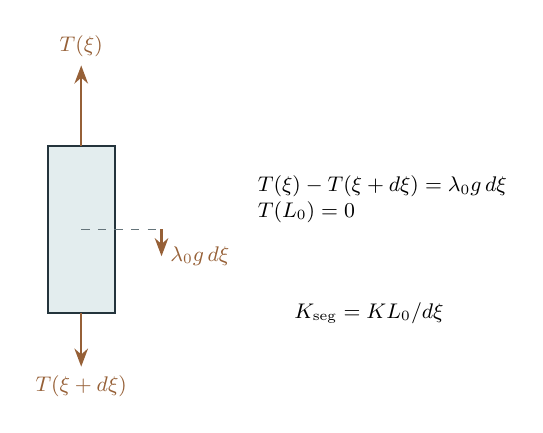
\begin{tikzpicture}[scale=.85,transform shape]

\fill[accent!12] (0,0) rectangle (1,-2.5);
\draw[object] (0,0) rectangle (1,-2.5);
\draw[force] (.5,0)--(.5,1.2) node[above] {$T(\xi)$};
\draw[force] (.5,-2.5)--(.5,-3.3) node[below] {$T(\xi+d\xi)$};
\draw[guide] (.5,-1.25)--(1.7,-1.25);
\draw[force,color=warm] (1.7,-1.25)--(1.7,-1.65) node[right] {$\lambda_0g\,d\xi$};
\node[align=left] at (5,-.8) {$T(\xi)-T(\xi+d\xi)=\lambda_0g\,d\xi$\\$T(L_0)=0$};
\node at (4.8,-2.5) {$K_{\rm seg}=KL_0/d\xi$};

\end{tikzpicture}
\figcaption{解图综三.3A\quad 一个材料微段的两端张力与重力；图中微段长度已经放大。}
\end{minipage}\end{center}
可把$\xi$想成刻在材料上的尺，读数一直跟随同一个材料点；外部固定的空间尺读数$x$记录该点在悬挂后的实际位置。自然长度微元$\mathrm d\xi$对应不变质量$\lambda_0\mathrm d\xi$，伸长后它占据$\mathrm dx=\mathrm d\xi+\mathrm d(\Delta\ell)$。因而求伸长与求密度共用同一个材料映射，长度微元随形变改变，质量保留。

解图综三.3A中，截面$\xi$以下的材料质量为$\lambda_0(L_0-\xi)$。它的重力由该截面张力承担，故
\[
T(\xi)=\lambda_0g(L_0-\xi).
\]
同样，图A的单个微段在静力平衡下满足$T(\xi)=T(\xi+\mathrm d\xi)+\lambda_0g\mathrm d\xi$，所以$\mathrm dT/\mathrm d\xi=-\lambda_0g$。从自由下端$T(L_0)=0$积分，也得到上述截面张力。上端张力为$mg$，下端为零，截面张力随其下方剩余材料质量从$mg$连续降到零。自然长度为$d\xi$的小段，其劲度系数为$KL_0/d\xi$。记恒定截面积为$S$，这个比例也可由杨氏模量导出：均匀端拉时应力为$F/S$、工程应变为$\Delta L/L_0$，故$E=FL_0/(S\Delta L)=KL_0/S$。轴向刚度$ES=KL_0$，对微段使用$T/S=E\,\mathrm d(\Delta\ell)/\mathrm d\xi$，即得微段劲度$ES/\mathrm d\xi$。因此该段伸长
\[
d(\Delta\ell)=\frac{T(\xi)}{KL_0}\,d\xi.
\]
将全杆看作这些串联小段并积分，得到
\[
\Delta L=\frac1{KL_0}\int_0^{L_0}\frac{mg}{L_0}(L_0-\xi)\,d\xi
=\boxed{\frac{mg}{2K}}.
\]
积分中的$\int_0^{L_0}(L_0-\xi)\mathrm d\xi=L_0^2/2$，与前面的$mg/(KL_0^2)$相乘，给$mg/(2K)$。上方小段承担下方全部材料重量，下方小段只承担更少重量，累积伸长按这种线性下降的张力积分。它等于把平均拉力$mg/2$作用于整根杆所得的伸长。这里的平均是对自然长度积分的结果，局部伸长使用各截面的实际张力。

为求密度，先保留一般参数$\alpha=mg/(KL_0)$。局部伸长比由原长加伸长给出，$\mathrm dx/\mathrm d\xi=1+T/(KL_0)=1+\alpha(1-\xi/L_0)$。它在上端为$1+\alpha$，在下端为1。把从上端到材料点的所有微段长度相加，得到该点的实际位置。从上端累积局部伸长，得
\[
x(\xi)=\int_0^\xi\left[1+\alpha\left(1-\frac{\eta}{L_0}\right)\right]d\eta
=(1+\alpha)\xi-\frac{\alpha\xi^2}{2L_0},
\quad
\frac{dx}{d\xi}=1+\alpha-\frac{\alpha\xi}{L_0}>0.
\]
\begin{center}\begin{minipage}{.98\linewidth}\centering
\begin{tikzpicture}[scale=.8,transform shape]
\draw[axis] (0,0)--(10.7,0) node[right] {$\xi/L_0$};
\draw[axis] (0,0)--(0,3.2) node[above] {$x/L_0$};\foreach \y/\lab in {0/0,0.9/.5,1.8/1,2.7/1.5}{\draw[thin] (0,\y)--(-.08,\y) node[left] {$\lab$};}
\node[above] at (5,3.5) {材料标签到空间位置的映射，题设$\alpha=1$};
\draw[traj] plot coordinates {(0.000000000,0.000000000) (0.083333333,0.029937500) (0.166666667,0.059750000) (0.250000000,0.089437500) (0.333333333,0.119000000) (0.416666667,0.148437500) (0.500000000,0.177750000) (0.583333333,0.206937500) (0.666666667,0.236000000) (0.750000000,0.264937500) (0.833333333,0.293750000) (0.916666667,0.322437500) (1.000000000,0.351000000) (1.083333333,0.379437500) (1.166666667,0.407750000) (1.250000000,0.435937500) (1.333333333,0.464000000) (1.416666667,0.491937500) (1.500000000,0.519750000) (1.583333333,0.547437500) (1.666666667,0.575000000) (1.750000000,0.602437500) (1.833333333,0.629750000) (1.916666667,0.656937500) (2.000000000,0.684000000) (2.083333333,0.710937500) (2.166666667,0.737750000) (2.250000000,0.764437500) (2.333333333,0.791000000) (2.416666667,0.817437500) (2.500000000,0.843750000) (2.583333333,0.869937500) (2.666666667,0.896000000) (2.750000000,0.921937500) (2.833333333,0.947750000) (2.916666667,0.973437500) (3.000000000,0.999000000) (3.083333333,1.024437500) (3.166666667,1.049750000) (3.250000000,1.074937500) (3.333333333,1.100000000) (3.416666667,1.124937500) (3.500000000,1.149750000) (3.583333333,1.174437500) (3.666666667,1.199000000) (3.750000000,1.223437500) (3.833333333,1.247750000) (3.916666667,1.271937500) (4.000000000,1.296000000) (4.083333333,1.319937500) (4.166666667,1.343750000) (4.250000000,1.367437500) (4.333333333,1.391000000) (4.416666667,1.414437500) (4.500000000,1.437750000) (4.583333333,1.460937500) (4.666666667,1.484000000) (4.750000000,1.506937500) (4.833333333,1.529750000) (4.916666667,1.552437500) (5.000000000,1.575000000) (5.083333333,1.597437500) (5.166666667,1.619750000) (5.250000000,1.641937500) (5.333333333,1.664000000) (5.416666667,1.685937500) (5.500000000,1.707750000) (5.583333333,1.729437500) (5.666666667,1.751000000) (5.750000000,1.772437500) (5.833333333,1.793750000) (5.916666667,1.814937500) (6.000000000,1.836000000) (6.083333333,1.856937500) (6.166666667,1.877750000) (6.250000000,1.898437500) (6.333333333,1.919000000) (6.416666667,1.939437500) (6.500000000,1.959750000) (6.583333333,1.979937500) (6.666666667,2.000000000) (6.750000000,2.019937500) (6.833333333,2.039750000) (6.916666667,2.059437500) (7.000000000,2.079000000) (7.083333333,2.098437500) (7.166666667,2.117750000) (7.250000000,2.136937500) (7.333333333,2.156000000) (7.416666667,2.174937500) (7.500000000,2.193750000) (7.583333333,2.212437500) (7.666666667,2.231000000) (7.750000000,2.249437500) (7.833333333,2.267750000) (7.916666667,2.285937500) (8.000000000,2.304000000) (8.083333333,2.321937500) (8.166666667,2.339750000) (8.250000000,2.357437500) (8.333333333,2.375000000) (8.416666667,2.392437500) (8.500000000,2.409750000) (8.583333333,2.426937500) (8.666666667,2.444000000) (8.750000000,2.460937500) (8.833333333,2.477750000) (8.916666667,2.494437500) (9.000000000,2.511000000) (9.083333333,2.527437500) (9.166666667,2.543750000) (9.250000000,2.559937500) (9.333333333,2.576000000) (9.416666667,2.591937500) (9.500000000,2.607750000) (9.583333333,2.623437500) (9.666666667,2.639000000) (9.750000000,2.654437500) (9.833333333,2.669750000) (9.916666667,2.684937500) (10.000000000,2.700000000)};
\node[below] at (0,-.12) {$0$};
\node[below] at (5,-.12) {$1/2$};
\node[below] at (10,-.12) {$1$};
\end{tikzpicture}
\figcaption{解图综三.3B\quad 材料标签到空间位置的映射，题设$\alpha=1$}
\end{minipage}\end{center}
解图综三.3B中同一质量元满足$\lambda(x)\,dx=\lambda_0\,d\xi$，所以
\[
\lambda(x(\xi))=\frac{\lambda_0}{1+\alpha-\alpha\xi/L_0}.
\]
相同质量在空间中被拉长得越多，单位空间长度内的质量就越少；因此密度除以局部伸长比。上式仍把密度对应到材料标签$\xi$，实际问题则使用固定尺读出的$x$。要把密度写成实际位置的函数，还须从映射中解出材料坐标。解二次方程，并取满足$x=0$时$\xi=0$的根，
\[
\xi=\frac{L_0}{\alpha}
\left[1+\alpha-\sqrt{(1+\alpha)^2-\frac{2\alpha x}{L_0}}\right].
\]
映射的导数始终为正，故$\xi$从0增加到$L_0$时，$x$从0单调增加到$L_0(1+\alpha/2)$，逆映射在这一区间唯一。代回后，分母$1+\alpha-\alpha\xi/L_0$恰变为二次根式中的平方根；其符号由正伸长比固定。代回雅可比，得到空间坐标下的分布
\[
\boxed{\lambda(x)=
\frac{m}{L_0\sqrt{(1+\alpha)^2-2\alpha x/L_0}}},
\quad 0\le x\le L_0(1+\alpha/2).
\]
所取根连续连接$\xi=0$的上端，并随$x$增加到$\xi=L_0$的下端。
\begin{center}\begin{minipage}{.98\linewidth}\centering
\begin{tikzpicture}[scale=.8,transform shape]
\draw[axis] (0,0)--(10.7,0) node[right] {$x/L_0$};
\draw[axis] (0,0)--(0,3.2) node[above] {$\lambda/\lambda_0$};
\node[above] at (5,3.5) {上端密度为$1/2$，下端恢复自然值1};
\draw[traj] plot coordinates {(0.000000000,1.400000000) (0.083333333,1.404395615) (0.166666667,1.408832895) (0.250000000,1.413312502) (0.333333333,1.417835114) (0.416666667,1.422401422) (0.500000000,1.427012136) (0.583333333,1.431667979) (0.666666667,1.436369693) (0.750000000,1.441118035) (0.833333333,1.445913783) (0.916666667,1.450757728) (1.000000000,1.455650686) (1.083333333,1.460593487) (1.166666667,1.465586983) (1.250000000,1.470632048) (1.333333333,1.475729575) (1.416666667,1.480880479) (1.500000000,1.486085699) (1.583333333,1.491346196) (1.666666667,1.496662955) (1.750000000,1.502036986) (1.833333333,1.507469326) (1.916666667,1.512961035) (2.000000000,1.518513205) (2.083333333,1.524126951) (2.166666667,1.529803421) (2.250000000,1.535543792) (2.333333333,1.541349271) (2.416666667,1.547221099) (2.500000000,1.553160549) (2.583333333,1.559168930) (2.666666667,1.565247584) (2.750000000,1.571397893) (2.833333333,1.577621275) (2.916666667,1.583919190) (3.000000000,1.590293136) (3.083333333,1.596744656) (3.166666667,1.603275336) (3.250000000,1.609886809) (3.333333333,1.616580754) (3.416666667,1.623358900) (3.500000000,1.630223027) (3.583333333,1.637174969) (3.666666667,1.644216615) (3.750000000,1.651349909) (3.833333333,1.658576858) (3.916666667,1.665899528) (4.000000000,1.673320053) (4.083333333,1.680840631) (4.166666667,1.688463530) (4.250000000,1.696191092) (4.333333333,1.704025734) (4.416666667,1.711969953) (4.500000000,1.720026327) (4.583333333,1.728197520) (4.666666667,1.736486284) (4.750000000,1.744895468) (4.833333333,1.753428015) (4.916666667,1.762086971) (5.000000000,1.770875490) (5.083333333,1.779796833) (5.166666667,1.788854382) (5.250000000,1.798051637) (5.333333333,1.807392228) (5.416666667,1.816879917) (5.500000000,1.826518605) (5.583333333,1.836312340) (5.666666667,1.846265326) (5.750000000,1.856381924) (5.833333333,1.866666667) (5.916666667,1.877124265) (6.000000000,1.887759615) (6.083333333,1.898577810) (6.166666667,1.909584151) (6.250000000,1.920784154) (6.333333333,1.932183566) (6.416666667,1.943788377) (6.500000000,1.955604828) (6.583333333,1.967639433) (6.666666667,1.979898987) (6.750000000,1.992390588) (6.833333333,2.005121647) (6.916666667,2.018099916) (7.000000000,2.031333500) (7.083333333,2.044830881) (7.166666667,2.058600942) (7.250000000,2.072652989) (7.333333333,2.086996779) (7.416666667,2.101642550) (7.500000000,2.116601049) (7.583333333,2.131883565) (7.666666667,2.147501969) (7.750000000,2.163468746) (7.833333333,2.179797044) (7.916666667,2.196500714) (8.000000000,2.213594362) (8.083333333,2.231093404) (8.166666667,2.249014121) (8.250000000,2.267373725) (8.333333333,2.286190427) (8.416666667,2.305483515) (8.500000000,2.325273436) (8.583333333,2.345581886) (8.666666667,2.366431913) (8.750000000,2.387848023) (8.833333333,2.409856304) (8.916666667,2.432484559) (9.000000000,2.455762454) (9.083333333,2.479721680) (9.166666667,2.504396135) (9.250000000,2.529822128) (9.333333333,2.556038602) (9.416666667,2.583087382) (9.500000000,2.611013463) (9.583333333,2.639865316) (9.666666667,2.669695250) (9.750000000,2.700559804) (9.833333333,2.732520204) (9.916666667,2.765642871) (10.000000000,2.800000000)};
\node[below] at (0,-.12) {$0$};
\node[below] at (6.666666666666667,-.12) {$1$};
\node[below] at (10,-.12) {$3/2$};
\node[left] at (0,1.4) {$1/2$};\node[left] at (0,2.8) {$1$};
\end{tikzpicture}
\figcaption{解图综三.3C\quad 上端密度为$1/2$，下端恢复自然值1}
\end{minipage}\end{center}
取题设$K=mg/L_0$，即$\alpha=1$，解图综三.3C中的曲线为
\[
\boxed{\lambda(x)=\frac{m}{L_0\sqrt{4-2x/L_0}}},
\qquad \boxed{0\le x\le\frac32L_0}.
\]
上端被拉得最疏，$\lambda(0)=m/(2L_0)$；下端张力为零，$\lambda(3L_0/2)=m/L_0$。积分实际空间密度得到总质量：
\[
\int_0^{3L_0/2}\lambda(x)\,dx
=m\left[-\sqrt{4-2x/L_0}\right]_0^{3L_0/2}=m.
\]
各段质量固定，伸长最大的上半部线密度较低。解图综三.3B 中材料坐标 $\xi=L_0/2$ 恰好平分质量；代入位置函数得 $x=L_0(1/2+3\alpha/8)$，比伸长后的长度中点 $L_0(1/2+\alpha/4)$ 低 $\alpha L_0/8$。题设 $\alpha=1$ 时上端工程应变为 $1$，这里按给定的线性拉伸关系和不变截面计算。
在一般参数下，空间下端的根式化为$\sqrt{(1+\alpha)^2-2\alpha(1+\alpha/2)}=1$，所以自由端恢复自然线密度；上端根式为$1+\alpha$，对应最大伸长比。

也可沿空间坐标理解静力平衡：$\mathrm dT/\mathrm dx=(\mathrm dT/\mathrm d\xi)/(\mathrm dx/\mathrm d\xi)=-g\lambda(x)$，表示上、下截面张力差支撑实际微段的重量。材料坐标中的常量质量密度与空间坐标中的变密度，通过相同伸长比相连。全长积分使用空间下端$3L_0/2$，上端和下端密度分别对应最大应变与零应变，三者都由映射的两端条件给出。



\Needspace{13\baselineskip}

\pdfbookmark[2]{第 4 题 阻尼振动、感应制动与受迫响应}{q4}

\section*{第 4 题\quad 阻尼振动、感应制动与受迫响应}\label{q:4}


（1）分别建立下列系统的运动方程，讨论能否振动及其条件。

甲：质量$m$、密度为水的$a$倍（$a>1$）的小球，用长$l$的轻质刚杆悬于水中，水对球的阻力为$-\gamma\boldsymbol v$。忽略杆的浮力、阻力，讨论小角度运动。

乙：间距$l$的水平平行导轨上有质量$m$的导体棒，与电阻$R$、自感$L$串联构成闭合回路。匀强磁场$B$垂直纸面向里。导轨和棒的电阻、摩擦忽略；初始棒向右以$v_0$运动，回路电流为零。分析速度和电流随时间的变化。

（2）对一般受迫振动方程
\[
\ddot x+2\beta\dot x+\omega_0^2x=h\cos pt
\]
（$\beta,\omega_0,h,p>0$），求完整解的结构和稳态振幅、相位，并说明暂态何时消失、振幅在何种频率达到最大。


\begin{center}\begin{minipage}{.98\linewidth}\centering
\begin{tikzpicture}[scale=.65,transform shape]

\draw[object] (-.7,0)--(.7,0);
\draw[guide] (0,0)--(0,-3.1);
\draw[object] (0,0)--(1.4,-2.4) node[midway,right] {$l$};
\fill[accent] (1.4,-2.4) circle (5pt) node[right] {$m$};
\draw[guide] (0,-.9) arc[start angle=-90,end angle=-59.74,radius=.9];
\node at (.45,-1.15) {$\theta$};
\draw[guide] (-1.5,-.8)--(2.7,-.8) node[right] {水面};

\begin{scope}[xshift=5.8cm]
\draw[object] (0,0)--(0,2)--(1.1,2);
\draw[object] (2.5,2)--(4,2)--(4,0)--(0,0);
\draw[object] (1.1,1.8) rectangle (2.5,2.2);
\node[above] at (1.8,2.2) {$L$};
\fill[white] (-.2,.5) rectangle (.2,1.5);
\draw[object] (-.2,.5) rectangle (.2,1.5);
\node[left] at (-.2,1) {$R$};
\draw[object,line width=2pt] (4,0)--(4,2);
\draw[motion] (4.2,1.3)--(5.3,1.3) node[right] {$v$};
\draw[motion] (3.7,.4)--(3.7,1.3) node[left] {$i$};
\node at (2,1) {$\otimes B$};
\draw[axis,<->] (5.8,0)--(5.8,2) node[midway,right] {$l$};
\end{scope}

\end{tikzpicture}
\figcaption{图综三.4\quad 水中轻杆摆与含串联电阻、自感的导体棒回路。}
\end{minipage}\end{center}

\Needspace{6\baselineskip}\subsection*{解答}


图综三.4中的轻杆可推可拉，摆球始终位于以悬点为圆心的圆周上。水的浮力为$mg/a$，因此重力与浮力的合力向下，大小$mg'=m(1-1/a)g$。
\begin{center}\begin{minipage}{.98\linewidth}\centering
\begin{tikzpicture}[scale=.85,transform shape]

\draw[object] (-.7,0)--(.7,0);
\draw[guide] (0,0)--(0,-3.1);
\draw[object] (0,0)--(1.4,-2.4) node[midway,right] {$l$};
\fill[accent] (1.4,-2.4) circle (5pt) node[right] {$m$};
\draw[guide] (0,-.9) arc[start angle=-90,end angle=-59.74,radius=.9];
\node at (.45,-1.15) {$\theta$};
\draw[guide] (-1.5,-.8)--(2.7,-.8) node[right] {水面};

\draw[force] (1.4,-2.4)--(1.4,-4) node[below] {$mg$};
\draw[force,color=warm] (1.65,-2.4)--(1.65,-1.25) node[right] {$mg/a$};
\draw[motion] (1.3,-2.5)--(.3,-3.08) node[below left] {$-\gamma\boldsymbol v$};
\node[align=left] at (5,-2) {$g'=(1-1/a)g$\\$\beta_1=\gamma/(2m)$\\$\omega_1^2=g'/l$};

\end{tikzpicture}
\figcaption{解图综三.4A\quad 重力、浮力及切向阻力；恢复力用有效重力，惯性仍用m。}
\end{minipage}\end{center}
密度比$a$使排开水的质量为$m/a$，所以浮力为$mg/a$。两力都沿竖直方向，它们关于悬点的力矩之差以同一个力臂$l\sin\theta$计算；球本身绕悬点的转动惯量仍是$ml^2$。

解图综三.4A以偏离竖直向下方向的$\theta$为坐标。阻力沿切线反向，大小$\gamma l|\dot\theta|$。关于悬点列力矩方程：
\[
ml^2\ddot\theta=-mg'l\sin\theta-\gamma l^2\dot\theta.
\]
小角度近似$\sin\theta\simeq\theta$，得到
\[
\ddot\theta+\frac{\gamma}{m}\dot\theta+\frac{g'}l\theta=0.
\]
阻力矩是阻力乘杆长，速度又等于$l\dot\theta$，所以阻力矩含$l^2$；除以惯性矩$ml^2$后阻尼率为$\gamma/m$。恢复力矩只含一个$l$，除后为$g'/l$，杆越长恢复频率越低。记$\beta_1=\gamma/(2m)$、$\omega_1=\sqrt{g'/l}$。特征根为
$-\beta_1\pm\sqrt{\beta_1^2-\omega_1^2}$。只有$\beta_1<\omega_1$时有衰减的正弦运动：
\[
\theta=e^{-\beta_1t}(C\cos\Omega_1t+D\sin\Omega_1t),\quad
\Omega_1=\sqrt{\omega_1^2-\beta_1^2}.
\]
故振动条件为
\[
\boxed{\gamma<2m\sqrt{\frac{(1-1/a)g}{l}}}
\quad\Longleftrightarrow\quad
\boxed{l<\frac{4m^2(1-1/a)g}{\gamma^2}}.
\]
等号为临界阻尼，大于临界值为过阻尼，均无往复的正弦振荡。浮力只改变恢复力，阻力项仍含小球本身的惯性质量$m$。
\begin{center}\begin{minipage}{.98\linewidth}\centering
\begin{tikzpicture}[scale=.85,transform shape]

\draw[object] (0,0)--(0,2)--(1.1,2);
\draw[object] (2.5,2)--(4,2)--(4,0)--(0,0);
\draw[object] (1.1,1.8) rectangle (2.5,2.2);
\node[above] at (1.8,2.2) {$L$};
\fill[white] (-.2,.5) rectangle (.2,1.5);
\draw[object] (-.2,.5) rectangle (.2,1.5);
\node[left] at (-.2,1) {$R$};
\draw[object,line width=2pt] (4,0)--(4,2);
\draw[motion] (4.2,1.3)--(5.3,1.3) node[right] {$v$};
\draw[motion] (3.7,.4)--(3.7,1.3) node[left] {$i$};
\node at (2,1) {$\otimes B$};
\draw[axis,<->] (5.8,0)--(5.8,2) node[midway,right] {$l$};

\draw[force] (3.8,.5)--(2.7,.5) node[midway,below] {$Bli$};
\node at (2.5,-1) {$L\dot i+Ri=Blv,\qquad m\dot v=-Bli$};
\node at (2.5,-2) {逆时针为正电流，初始$i=0$};

\end{tikzpicture}
\figcaption{解图综三.4B\quad 回路正向与棒的磁力；电感允许能量先储存再返回机械运动。}
\end{minipage}\end{center}
解图综三.4B将逆时针电流$i$定为正：右侧棒内正电流向上，所受磁力向左。运动电动势使这一方向的电流增大，回路和棒分别满足
\[
L\dot i+Ri=Blv,\qquad m\dot v=-Bli.
\]
由机械方程先得$i=-m\dot v/(Bl)$，再对时间求导得到$\dot i=-m\ddot v/(Bl)$。代入回路式后，$-Lm\ddot v/(Bl)-Rm\dot v/(Bl)=Blv$，乘$-Bl/(mL)$并移项，消去$i$，得到
\[
\boxed{\ddot v+\frac RL\dot v+\frac{B^2l^2}{mL}v=0},\qquad
v(0)=v_0,\quad\dot v(0)=0.
\]
两个一阶状态分别记录棒的机械运动和电感储能，初态$v_0,0$给$\dot i(0)=Blv_0/L$、$\dot v(0)=0$。电流先从零增长，随后磁力才逐渐制动棒。自感使电流不能瞬时跳变，故初始磁力与初始加速度均为零。令
$\beta_2=R/(2L)$、$\omega_2=Bl/\sqrt{mL}$，临界电阻为
\[
\boxed{R_c=2Bl\sqrt{L/m}}.
\]
在$0<R<R_c$时，$\Omega_2=\sqrt{\omega_2^2-\beta_2^2}$，
\[
\boxed{v=v_0e^{-\beta_2t}
\left(\cos\Omega_2t+\frac{\beta_2}{\Omega_2}\sin\Omega_2t\right)},\qquad
\boxed{i=\frac{Blv_0}{L\Omega_2}e^{-\beta_2t}\sin\Omega_2t}.
\]
欠阻尼速度表达式中的余弦、正弦系数由$v(0)=v_0,\dot v(0)=0$确定，电流则由$-m\dot v/(Bl)$求出，求导时两个余弦项相消，只留下正弦项。速度过零后，电感中的原方向电流还可持续一段时间。棒可反向运动，磁场能在机械能与电感能之间交换。在$R=R_c$时
\[
v=v_0(1+\beta_2t)e^{-\beta_2t},\qquad
i=\frac{Blv_0}{L}t e^{-\beta_2t}.
\]
在$R>R_c$时，令$q=\sqrt{\beta_2^2-\omega_2^2}$，则
\[
v=v_0e^{-\beta_2t}
\left(\cosh qt+\frac{\beta_2}{q}\sinh qt\right),\qquad
i=\frac{Blv_0}{Lq}e^{-\beta_2t}\sinh qt.
\]
\begin{center}\begin{minipage}{.98\linewidth}\centering
\begin{tikzpicture}[scale=.8,transform shape]
\draw[axis] (0,0)--(10.7,0) node[right] {$\omega_2t$};
\draw[axis] (0,0)--(0,3.2) node[above] {$v/v_0$};\foreach \y/\lab in {0.38/-.2,2.66/1}{\draw[thin] (0,\y)--(-.08,\y) node[left] {$\lab$};}
\node[above] at (5,3.5) {实线欠阻尼，细线临界，虚线过阻尼；各曲线初始斜率为零};
\draw[traj] plot coordinates {(0.000000000,2.660000000) (0.062500000,2.657649062) (0.125000000,2.650694911) (0.187500000,2.639290716) (0.250000000,2.623596078) (0.312500000,2.603776443) (0.375000000,2.580002527) (0.437500000,2.552449737) (0.500000000,2.521297599) (0.562500000,2.486729200) (0.625000000,2.448930623) (0.687500000,2.408090409) (0.750000000,2.364399016) (0.812500000,2.318048292) (0.875000000,2.269230964) (0.937500000,2.218140138) (1.000000000,2.164968809) (1.062500000,2.109909392) (1.125000000,2.053153265) (1.187500000,1.994890328) (1.250000000,1.935308577) (1.312500000,1.874593701) (1.375000000,1.812928691) (1.437500000,1.750493469) (1.500000000,1.687464536) (1.562500000,1.624014639) (1.625000000,1.560312455) (1.687500000,1.496522298) (1.750000000,1.432803843) (1.812500000,1.369311868) (1.875000000,1.306196020) (1.937500000,1.243600597) (2.000000000,1.181664349) (2.062500000,1.120520305) (2.125000000,1.060295611) (2.187500000,1.001111389) (2.250000000,0.943082623) (2.312500000,0.886318050) (2.375000000,0.830920084) (2.437500000,0.776984745) (2.500000000,0.724601613) (2.562500000,0.673853800) (2.625000000,0.624817935) (2.687500000,0.577564165) (2.750000000,0.532156177) (2.812500000,0.488651232) (2.875000000,0.447100211) (2.937500000,0.407547679) (3.000000000,0.370031966) (3.062500000,0.334585251) (3.125000000,0.301233668) (3.187500000,0.269997421) (3.250000000,0.240890907) (3.312500000,0.213922854) (3.375000000,0.189096465) (3.437500000,0.166409577) (3.500000000,0.145854820) (3.562500000,0.127419794) (3.625000000,0.111087245) (3.687500000,0.096835252) (3.750000000,0.084637418) (3.812500000,0.074463071) (3.875000000,0.066277459) (3.937500000,0.060041963) (4.000000000,0.055714301) (4.062500000,0.053248745) (4.125000000,0.052596333) (4.187500000,0.053705085) (4.250000000,0.056520220) (4.312500000,0.060984375) (4.375000000,0.067037821) (4.437500000,0.074618684) (4.500000000,0.083663152) (4.562500000,0.094105701) (4.625000000,0.105879296) (4.687500000,0.118915609) (4.750000000,0.133145221) (4.812500000,0.148497826) (4.875000000,0.164902431) (4.937500000,0.182287551) (5.000000000,0.200581398) (5.062500000,0.219712070) (5.125000000,0.239607728) (5.187500000,0.260196773) (5.250000000,0.281408014) (5.312500000,0.303170835) (5.375000000,0.325415344) (5.437500000,0.348072532) (5.500000000,0.371074412) (5.562500000,0.394354159) (5.625000000,0.417846236) (5.687500000,0.441486523) (5.750000000,0.465212429) (5.812500000,0.488963001) (5.875000000,0.512679028) (5.937500000,0.536303133) (6.000000000,0.559779863) (6.062500000,0.583055764) (6.125000000,0.606079459) (6.187500000,0.628801708) (6.250000000,0.651175471) (6.312500000,0.673155954) (6.375000000,0.694700657) (6.437500000,0.715769408) (6.500000000,0.736324396) (6.562500000,0.756330189) (6.625000000,0.775753758) (6.687500000,0.794564482) (6.750000000,0.812734156) (6.812500000,0.830236984) (6.875000000,0.847049576) (6.937500000,0.863150934) (7.000000000,0.878522431) (7.062500000,0.893147786) (7.125000000,0.907013039) (7.187500000,0.920106513) (7.250000000,0.932418776) (7.312500000,0.943942600) (7.375000000,0.954672911) (7.437500000,0.964606739) (7.500000000,0.973743162) (7.562500000,0.982083251) (7.625000000,0.989630005) (7.687500000,0.996388286) (7.750000000,1.002364757) (7.812500000,1.007567808) (7.875000000,1.012007484) (7.937500000,1.015695416) (8.000000000,1.018644738) (8.062500000,1.020870019) (8.125000000,1.022387177) (8.187500000,1.023213404) (8.250000000,1.023367087) (8.312500000,1.022867724) (8.375000000,1.021735844) (8.437500000,1.019992929) (8.500000000,1.017661329) (8.562500000,1.014764183) (8.625000000,1.011325340) (8.687500000,1.007369277) (8.750000000,1.002921021) (8.812500000,0.998006072) (8.875000000,0.992650325) (8.937500000,0.986879996) (9.000000000,0.980721546) (9.062500000,0.974201610) (9.125000000,0.967346926) (9.187500000,0.960184266) (9.250000000,0.952740369) (9.312500000,0.945041876) (9.375000000,0.937115268) (9.437500000,0.928986806) (9.500000000,0.920682470) (9.562500000,0.912227906) (9.625000000,0.903648373) (9.687500000,0.894968689) (9.750000000,0.886213187) (9.812500000,0.877405667) (9.875000000,0.868569354) (9.937500000,0.859726857) (10.000000000,0.850900131)};
\draw[thin,color=black] plot coordinates {(0.000000000,2.660000000) (0.062500000,2.657702702) (0.125000000,2.651110204) (0.187500000,2.640646928) (0.250000000,2.626706117) (0.312500000,2.609651860) (0.375000000,2.589821005) (0.437500000,2.567524950) (0.500000000,2.543051322) (0.562500000,2.516665558) (0.625000000,2.488612380) (0.687500000,2.459117192) (0.750000000,2.428387374) (0.812500000,2.396613510) (0.875000000,2.363970531) (0.937500000,2.330618788) (1.000000000,2.296705057) (1.062500000,2.262363486) (1.125000000,2.227716472) (1.187500000,2.192875492) (1.250000000,2.157941876) (1.312500000,2.123007533) (1.375000000,2.088155624) (1.437500000,2.053461203) (1.500000000,2.018991806) (1.562500000,1.984808007) (1.625000000,1.950963936) (1.687500000,1.917507764) (1.750000000,1.884482156) (1.812500000,1.851924691) (1.875000000,1.819868261) (1.937500000,1.788341433) (2.000000000,1.757368799) (2.062500000,1.726971290) (2.125000000,1.697166478) (2.187500000,1.667968855) (2.250000000,1.639390085) (2.312500000,1.611439256) (2.375000000,1.584123092) (2.437500000,1.557446171) (2.500000000,1.531411114) (2.562500000,1.506018766) (2.625000000,1.481268362) (2.687500000,1.457157684) (2.750000000,1.433683203) (2.812500000,1.410840212) (2.875000000,1.388622950) (2.937500000,1.367024718) (3.000000000,1.346037978) (3.062500000,1.325654460) (3.125000000,1.305865241) (3.187500000,1.286660837) (3.250000000,1.268031275) (3.312500000,1.249966163) (3.375000000,1.232454755) (3.437500000,1.215486011) (3.500000000,1.199048652) (3.562500000,1.183131207) (3.625000000,1.167722061) (3.687500000,1.152809493) (3.750000000,1.138381720) (3.812500000,1.124426923) (3.875000000,1.110933287) (3.937500000,1.097889020) (4.000000000,1.085282388) (4.062500000,1.073101728) (4.125000000,1.061335478) (4.187500000,1.049972187) (4.250000000,1.039000537) (4.312500000,1.028409356) (4.375000000,1.018187628) (4.437500000,1.008324510) (4.500000000,0.998809334) (4.562500000,0.989631623) (4.625000000,0.980781091) (4.687500000,0.972247656) (4.750000000,0.964021439) (4.812500000,0.956092771) (4.875000000,0.948452196) (4.937500000,0.941090470) (5.000000000,0.933998569) (5.062500000,0.927167685) (5.125000000,0.920589225) (5.187500000,0.914254815) (5.250000000,0.908156299) (5.312500000,0.902285733) (5.375000000,0.896635389) (5.437500000,0.891197750) (5.500000000,0.885965507) (5.562500000,0.880931561) (5.625000000,0.876089014) (5.687500000,0.871431170) (5.750000000,0.866951532) (5.812500000,0.862643797) (5.875000000,0.858501851) (5.937500000,0.854519770) (6.000000000,0.850691812) (6.062500000,0.847012416) (6.125000000,0.843476196) (6.187500000,0.840077938) (6.250000000,0.836812596) (6.312500000,0.833675288) (6.375000000,0.830661293) (6.437500000,0.827766044) (6.500000000,0.824985129) (6.562500000,0.822314281) (6.625000000,0.819749379) (6.687500000,0.817286442) (6.750000000,0.814921624) (6.812500000,0.812651214) (6.875000000,0.810471627) (6.937500000,0.808379405) (7.000000000,0.806371211) (7.062500000,0.804443824) (7.125000000,0.802594140) (7.187500000,0.800819164) (7.250000000,0.799116007) (7.312500000,0.797481888) (7.375000000,0.795914122) (7.437500000,0.794410124) (7.500000000,0.792967404) (7.562500000,0.791583562) (7.625000000,0.790256286) (7.687500000,0.788983350) (7.750000000,0.787762611) (7.812500000,0.786592006) (7.875000000,0.785469547) (7.937500000,0.784393324) (8.000000000,0.783361495) (8.062500000,0.782372291) (8.125000000,0.781424008) (8.187500000,0.780515008) (8.250000000,0.779643714) (8.312500000,0.778808611) (8.375000000,0.778008241) (8.437500000,0.777241202) (8.500000000,0.776506148) (8.562500000,0.775801782) (8.625000000,0.775126859) (8.687500000,0.774480184) (8.750000000,0.773860606) (8.812500000,0.773267020) (8.875000000,0.772698365) (8.937500000,0.772153620) (9.000000000,0.771631807) (9.062500000,0.771131984) (9.125000000,0.770653246) (9.187500000,0.770194728) (9.250000000,0.769755594) (9.312500000,0.769335045) (9.375000000,0.768932313) (9.437500000,0.768546659) (9.500000000,0.768177376) (9.562500000,0.767823785) (9.625000000,0.767485233) (9.687500000,0.767161095) (9.750000000,0.766850769) (9.812500000,0.766553679) (9.875000000,0.766269273) (9.937500000,0.765997020) (10.000000000,0.765736411)};
\draw[dashed,thick,color=warm] plot coordinates {(0.000000000,2.660000000) (0.062500000,2.657739893) (0.125000000,2.651389852) (0.187500000,2.641534309) (0.250000000,2.628684430) (0.312500000,2.613287125) (0.375000000,2.595732970) (0.437500000,2.576363140) (0.500000000,2.555475502) (0.562500000,2.533329957) (0.625000000,2.510153121) (0.687500000,2.486142441) (0.750000000,2.461469793) (0.812500000,2.436284652) (0.875000000,2.410716858) (0.937500000,2.384879058) (1.000000000,2.358868831) (1.062500000,2.332770566) (1.125000000,2.306657102) (1.187500000,2.280591166) (1.250000000,2.254626639) (1.312500000,2.228809659) (1.375000000,2.203179598) (1.437500000,2.177769907) (1.500000000,2.152608869) (1.562500000,2.127720247) (1.625000000,2.103123864) (1.687500000,2.078836103) (1.750000000,2.054870348) (1.812500000,2.031237373) (1.875000000,2.007945677) (1.937500000,1.985001783) (2.000000000,1.962410501) (2.062500000,1.940175148) (2.125000000,1.918297757) (2.187500000,1.896779244) (2.250000000,1.875619567) (2.312500000,1.854817855) (2.375000000,1.834372529) (2.437500000,1.814281400) (2.500000000,1.794541765) (2.562500000,1.775150481) (2.625000000,1.756104032) (2.687500000,1.737398595) (2.750000000,1.719030084) (2.812500000,1.700994203) (2.875000000,1.683286482) (2.937500000,1.665902310) (3.000000000,1.648836971) (3.062500000,1.632085661) (3.125000000,1.615643521) (3.187500000,1.599505648) (3.250000000,1.583667117) (3.312500000,1.568122995) (3.375000000,1.552868350) (3.437500000,1.537898269) (3.500000000,1.523207859) (3.562500000,1.508792263) (3.625000000,1.494646659) (3.687500000,1.480766274) (3.750000000,1.467146381) (3.812500000,1.453782307) (3.875000000,1.440669440) (3.937500000,1.427803221) (4.000000000,1.415179160) (4.062500000,1.402792826) (4.125000000,1.390639855) (4.187500000,1.378715949) (4.250000000,1.367016877) (4.312500000,1.355538476) (4.375000000,1.344276650) (4.437500000,1.333227371) (4.500000000,1.322386679) (4.562500000,1.311750681) (4.625000000,1.301315551) (4.687500000,1.291077532) (4.750000000,1.281032929) (4.812500000,1.271178115) (4.875000000,1.261509529) (4.937500000,1.252023670) (5.000000000,1.242717104) (5.062500000,1.233586458) (5.125000000,1.224628420) (5.187500000,1.215839740) (5.250000000,1.207217225) (5.312500000,1.198757745) (5.375000000,1.190458223) (5.437500000,1.182315644) (5.500000000,1.174327045) (5.562500000,1.166489521) (5.625000000,1.158800218) (5.687500000,1.151256339) (5.750000000,1.143855136) (5.812500000,1.136593914) (5.875000000,1.129470030) (5.937500000,1.122480887) (6.000000000,1.115623940) (6.062500000,1.108896689) (6.125000000,1.102296684) (6.187500000,1.095821520) (6.250000000,1.089468835) (6.312500000,1.083236316) (6.375000000,1.077121688) (6.437500000,1.071122724) (6.500000000,1.065237237) (6.562500000,1.059463080) (6.625000000,1.053798148) (6.687500000,1.048240375) (6.750000000,1.042787736) (6.812500000,1.037438241) (6.875000000,1.032189940) (6.937500000,1.027040919) (7.000000000,1.021989300) (7.062500000,1.017033241) (7.125000000,1.012170935) (7.187500000,1.007400607) (7.250000000,1.002720519) (7.312500000,0.998128963) (7.375000000,0.993624265) (7.437500000,0.989204782) (7.500000000,0.984868902) (7.562500000,0.980615043) (7.625000000,0.976441654) (7.687500000,0.972347213) (7.750000000,0.968330227) (7.812500000,0.964389230) (7.875000000,0.960522784) (7.937500000,0.956729480) (8.000000000,0.953007934) (8.062500000,0.949356789) (8.125000000,0.945774712) (8.187500000,0.942260398) (8.250000000,0.938812564) (8.312500000,0.935429953) (8.375000000,0.932111331) (8.437500000,0.928855487) (8.500000000,0.925661234) (8.562500000,0.922527408) (8.625000000,0.919452864) (8.687500000,0.916436481) (8.750000000,0.913477159) (8.812500000,0.910573820) (8.875000000,0.907725402) (8.937500000,0.904930869) (9.000000000,0.902189200) (9.062500000,0.899499395) (9.125000000,0.896860473) (9.187500000,0.894271473) (9.250000000,0.891731448) (9.312500000,0.889239473) (9.375000000,0.886794640) (9.437500000,0.884396055) (9.500000000,0.882042844) (9.562500000,0.879734150) (9.625000000,0.877469129) (9.687500000,0.875246956) (9.750000000,0.873066820) (9.812500000,0.870927925) (9.875000000,0.868829492) (9.937500000,0.866770756) (10.000000000,0.864750965)};
\node[below] at (0,-.12) {$0$};
\node[below] at (5,-.12) {$4$};
\node[below] at (10,-.12) {$8$};
\draw[dotted] (0,.76)--(10,.76);\node[left] at (0,.76) {$0$};
\end{tikzpicture}
\figcaption{解图综三.4C\quad 实线欠阻尼，细线临界，虚线过阻尼；各曲线初始斜率为零}
\end{minipage}\end{center}
解图综三.4C比较三种阻尼。将力学方程乘$v$、回路方程乘$i$并相加，
\[
\frac d{dt}\left(\frac12mv^2+\frac12Li^2\right)=-Ri^2.
\]
这一步的耦合功率$Blvi$在两式中一正一负，表示机械能与磁能之间的交换；相加后只剩电阻热耗散。对$R>0$，最终$v,i\to0$；从动力学方程积分得
$\int_0^\infty i\,dt=mv_0/(Bl)$，再积分回路方程，左端电感项为$L[i(\infty)-i(0)]=0$，因此$Bl\Delta x=R\int_0^\infty i\,\mathrm dt$。把前式的电流积分代入，便有
\[
\boxed{\Delta x=\int_0^\infty v\,dt=\frac{Rm v_0}{B^2l^2}}.
\]
这里速度按方向带符号积分，得到净位移；总路程使用$|v|$的积分。若$R=0$，系统不衰减，
$v=v_0\cos\omega_2t$，$i=Blv_0\sin\omega_2t/(L\omega_2)$；
零电阻下位移随时间周期变化，前述净位移积分用于$R>0$的衰减过程。

水中摆和导体棒分别使用角度与速度作振子变量，它们的特征方程结构相同，但变量代表的物理对象不同。以下用一般位移坐标$x$讨论外力驱动，令$h$为驱动力幅值除以质量。

一般受迫方程的解等于一个特解加齐次解。先令
$x_s=A\cos(pt-\delta)$，代入后分别比较$\cos pt,\sin pt$的系数：
\[
A[(\omega_0^2-p^2)\cos\delta+2\beta p\sin\delta]=h,
\]
\[
A[(\omega_0^2-p^2)\sin\delta-2\beta p\cos\delta]=0.
\]
将两式分别平方再相加时，含$\sin\delta\cos\delta$的交叉项相消，留下$A^2[(\omega_0^2-p^2)^2+4\beta^2p^2]=h^2$。同时由两方程得到$\cos\delta=(\omega_0^2-p^2)/D$、$\sin\delta=2\beta p/D$，$D$为分母的正平方根。由$A>0$取正振幅，并按图D中的两分量确定相位，得到
\[
\boxed{A=\frac{h}{\sqrt{(\omega_0^2-p^2)^2+4\beta^2p^2}}},
\quad
\boxed{\delta=\operatorname{atan2}(2\beta p,\omega_0^2-p^2)\in(0,\pi)}.
\]
\begin{center}\begin{minipage}{.98\linewidth}\centering
\begin{tikzpicture}[scale=.8,transform shape]
\draw[axis] (-2.5,0)--(2.4,0) node[right] {$\omega_0^2-p^2$};\draw[axis] (0,-.3)--(0,2.6) node[above] {$2\beta p$};\draw[motion] (0,0)--(1.125,.45) node[above right] {低频};\draw[force] (0,0)--(-1.875,1.35) node[above left] {高频};\draw (.65,0) arc(0:144.246113:.65);\node at (-.6,.9) {$\delta$};\node[align=left] at (1,-1.2) {相同坐标比例\qquad $0<\delta<\pi$};
\end{tikzpicture}
\figcaption{解图综三.4D\quad 动态刚度的两个相位示例，位移滞后角按矢量象限确定}
\end{minipage}\end{center}
解图综三.4D中的相位向量横分量为$\omega_0^2-p^2$，纵分量为$2\beta p>0$。
低频时$\delta<\pi/2$，$p=\omega_0$时$\delta=\pi/2$，高频时$\delta>\pi/2$。
相位按两分量的符号进入相应象限。

\begin{center}\begin{minipage}{.98\linewidth}\centering
\begin{tikzpicture}[scale=.8,transform shape]
\draw[axis] (0,0)--(10.7,0) node[right] {$\omega_0t$};
\draw[axis] (0,0)--(0,3.2) node[above] {$x\omega_0^2/h$};\foreach \y/\lab in {0.56/-1,2.16/1,2.96/2}{\draw[thin] (0,\y)--(-.08,\y) node[left] {$\lab$};}
\node[above] at (5,3.5) {取$\beta/\omega_0=.3,p/\omega_0=1.2$；实线完整运动，虚线周期特解};
\draw[traj] plot coordinates {(0.000000000,1.360000000) (0.041666667,1.361541923) (0.083333333,1.366077212) (0.125000000,1.373452460) (0.166666667,1.383491987) (0.208333333,1.395999570) (0.250000000,1.410760291) (0.291666667,1.427542471) (0.333333333,1.446099701) (0.375000000,1.466172927) (0.416666667,1.487492601) (0.458333333,1.509780870) (0.500000000,1.532753789) (0.541666667,1.556123552) (0.583333333,1.579600716) (0.625000000,1.602896414) (0.666666667,1.625724536) (0.708333333,1.647803868) (0.750000000,1.668860179) (0.791666667,1.688628229) (0.833333333,1.706853711) (0.875000000,1.723295091) (0.916666667,1.737725346) (0.958333333,1.749933593) (1.000000000,1.759726596) (1.041666667,1.766930139) (1.083333333,1.771390258) (1.125000000,1.772974339) (1.166666667,1.771572052) (1.208333333,1.767096138) (1.250000000,1.759483033) (1.291666667,1.748693326) (1.333333333,1.734712062) (1.375000000,1.717548866) (1.416666667,1.697237916) (1.458333333,1.673837739) (1.500000000,1.647430853) (1.541666667,1.618123248) (1.583333333,1.586043709) (1.625000000,1.551342991) (1.666666667,1.514192855) (1.708333333,1.474784953) (1.750000000,1.433329599) (1.791666667,1.390054403) (1.833333333,1.345202805) (1.875000000,1.299032496) (1.916666667,1.251813754) (1.958333333,1.203827685) (2.000000000,1.155364413) (2.041666667,1.106721184) (2.083333333,1.058200450) (2.125000000,1.010107892) (2.166666667,0.962750438) (2.208333333,0.916434260) (2.250000000,0.871462777) (2.291666667,0.828134666) (2.333333333,0.786741910) (2.375000000,0.747567871) (2.416666667,0.710885425) (2.458333333,0.676955146) (2.500000000,0.646023577) (2.541666667,0.618321574) (2.583333333,0.594062745) (2.625000000,0.573441997) (2.666666667,0.556634189) (2.708333333,0.543792909) (2.750000000,0.535049379) (2.791666667,0.530511491) (2.833333333,0.530262990) (2.875000000,0.534362792) (2.916666667,0.542844466) (2.958333333,0.555715856) (3.000000000,0.572958865) (3.041666667,0.594529398) (3.083333333,0.620357456) (3.125000000,0.650347394) (3.166666667,0.684378328) (3.208333333,0.722304704) (3.250000000,0.763957008) (3.291666667,0.809142631) (3.333333333,0.857646870) (3.375000000,0.909234065) (3.416666667,0.963648870) (3.458333333,1.020617639) (3.500000000,1.079849930) (3.541666667,1.141040115) (3.583333333,1.203869082) (3.625000000,1.268006025) (3.666666667,1.333110310) (3.708333333,1.398833403) (3.750000000,1.464820856) (3.791666667,1.530714329) (3.833333333,1.596153646) (3.875000000,1.660778866) (3.916666667,1.724232365) (3.958333333,1.786160903) (4.000000000,1.846217683) (4.041666667,1.904064369) (4.083333333,1.959373071) (4.125000000,2.011828269) (4.166666667,2.061128673) (4.208333333,2.106989012) (4.250000000,2.149141730) (4.291666667,2.187338587) (4.333333333,2.221352156) (4.375000000,2.250977199) (4.416666667,2.276031927) (4.458333333,2.296359126) (4.500000000,2.311827141) (4.541666667,2.322330726) (4.583333333,2.327791731) (4.625000000,2.328159655) (4.666666667,2.323412022) (4.708333333,2.313554615) (4.750000000,2.298621539) (4.791666667,2.278675125) (4.833333333,2.253805676) (4.875000000,2.224131052) (4.916666667,2.189796092) (4.958333333,2.150971888) (5.000000000,2.107854904) (5.041666667,2.060665954) (5.083333333,2.009649030) (5.125000000,1.955070004) (5.166666667,1.897215202) (5.208333333,1.836389854) (5.250000000,1.772916439) (5.291666667,1.707132925) (5.333333333,1.639390921) (5.375000000,1.570053745) (5.416666667,1.499494422) (5.458333333,1.428093625) (5.500000000,1.356237569) (5.541666667,1.284315865) (5.583333333,1.212719355) (5.625000000,1.141837938) (5.666666667,1.072058388) (5.708333333,1.003762194) (5.750000000,0.937323425) (5.791666667,0.873106630) (5.833333333,0.811464787) (5.875000000,0.752737316) (5.916666667,0.697248166) (5.958333333,0.645303984) (6.000000000,0.597192375) (6.041666667,0.553180271) (6.083333333,0.513512415) (6.125000000,0.478409957) (6.166666667,0.448069193) (6.208333333,0.422660431) (6.250000000,0.402327011) (6.291666667,0.387184463) (6.333333333,0.377319832) (6.375000000,0.372791150) (6.416666667,0.373627082) (6.458333333,0.379826721) (6.500000000,0.391359564) (6.541666667,0.408165645) (6.583333333,0.430155829) (6.625000000,0.457212282) (6.666666667,0.489189090) (6.708333333,0.525913043) (6.750000000,0.567184569) (6.791666667,0.612778818) (6.833333333,0.662446887) (6.875000000,0.715917185) (6.916666667,0.772896918) (6.958333333,0.833073700) (7.000000000,0.896117278) (7.041666667,0.961681348) (7.083333333,1.029405471) (7.125000000,1.098917066) (7.166666667,1.169833476) (7.208333333,1.241764085) (7.250000000,1.314312487) (7.291666667,1.387078691) (7.333333333,1.459661335) (7.375000000,1.531659929) (7.416666667,1.602677074) (7.458333333,1.672320682) (7.500000000,1.740206155) (7.541666667,1.805958534) (7.583333333,1.869214587) (7.625000000,1.929624838) (7.666666667,1.986855518) (7.708333333,2.040590431) (7.750000000,2.090532718) (7.791666667,2.136406522) (7.833333333,2.177958530) (7.875000000,2.214959390) (7.916666667,2.247205001) (7.958333333,2.274517652) (8.000000000,2.296747025) (8.041666667,2.313771038) (8.083333333,2.325496535) (8.125000000,2.331859809) (8.166666667,2.332826967) (8.208333333,2.328394124) (8.250000000,2.318587434) (8.291666667,2.303462945) (8.333333333,2.283106299) (8.375000000,2.257632252) (8.416666667,2.227184043) (8.458333333,2.191932601) (8.500000000,2.152075590) (8.541666667,2.107836313) (8.583333333,2.059462469) (8.625000000,2.007224773) (8.666666667,1.951415444) (8.708333333,1.892346582) (8.750000000,1.830348422) (8.791666667,1.765767492) (8.833333333,1.698964682) (8.875000000,1.630313228) (8.916666667,1.560196625) (8.958333333,1.489006489) (9.000000000,1.417140368) (9.041666667,1.344999523) (9.083333333,1.272986680) (9.125000000,1.201503789) (9.166666667,1.130949768) (9.208333333,1.061718280) (9.250000000,0.994195529) (9.291666667,0.928758104) (9.333333333,0.865770869) (9.375000000,0.805584930) (9.416666667,0.748535666) (9.458333333,0.694940856) (9.500000000,0.645098903) (9.541666667,0.599287166) (9.583333333,0.557760410) (9.625000000,0.520749377) (9.666666667,0.488459506) (9.708333333,0.461069775) (9.750000000,0.438731709) (9.791666667,0.421568529) (9.833333333,0.409674467) (9.875000000,0.403114243) (9.916666667,0.401922699) (9.958333333,0.406104614) (10.000000000,0.415634676)};
\draw[dashed,thick,color=warm] plot coordinates {(0.000000000,0.865617978) (0.041666667,0.927625067) (0.083333333,0.992063125) (0.125000000,1.058569858) (0.166666667,1.126771341) (0.208333333,1.196284121) (0.250000000,1.266717370) (0.291666667,1.337675089) (0.333333333,1.408758326) (0.375000000,1.479567426) (0.416666667,1.549704275) (0.458333333,1.618774537) (0.500000000,1.686389875) (0.541666667,1.752170130) (0.583333333,1.815745462) (0.625000000,1.876758427) (0.666666667,1.934865989) (0.708333333,1.989741444) (0.750000000,2.041076264) (0.791666667,2.088581826) (0.833333333,2.131991036) (0.875000000,2.171059831) (0.916666667,2.205568552) (0.958333333,2.235323180) (1.000000000,2.260156422) (1.041666667,2.279928658) (1.083333333,2.294528720) (1.125000000,2.303874521) (1.166666667,2.307913517) (1.208333333,2.306622998) (1.250000000,2.300010220) (1.291666667,2.288112363) (1.333333333,2.270996320) (1.375000000,2.248758325) (1.416666667,2.221523407) (1.458333333,2.189444691) (1.500000000,2.152702535) (1.541666667,2.111503517) (1.583333333,2.066079273) (1.625000000,2.016685195) (1.666666667,1.963598994) (1.708333333,1.907119139) (1.750000000,1.847563182) (1.791666667,1.785265967) (1.833333333,1.720577752) (1.875000000,1.653862237) (1.916666667,1.585494523) (1.958333333,1.515858996) (2.000000000,1.445347173) (2.041666667,1.374355497) (2.083333333,1.303283110) (2.125000000,1.232529605) (2.166666667,1.162492786) (2.208333333,1.093566423) (2.250000000,1.026138048) (2.291666667,0.960586765) (2.333333333,0.897281129) (2.375000000,0.836577067) (2.416666667,0.778815880) (2.458333333,0.724322320) (2.500000000,0.673402772) (2.541666667,0.626343523) (2.583333333,0.583409158) (2.625000000,0.544841069) (2.666666667,0.510856100) (2.708333333,0.481645327) (2.750000000,0.457372983) (2.791666667,0.438175537) (2.833333333,0.424160924) (2.875000000,0.415407938) (2.916666667,0.411965792) (2.958333333,0.413853839) (3.000000000,0.421061465) (3.041666667,0.433548144) (3.083333333,0.451243673) (3.125000000,0.474048560) (3.166666667,0.501834589) (3.208333333,0.534445536) (3.250000000,0.571698050) (3.291666667,0.613382684) (3.333333333,0.659265073) (3.375000000,0.709087249) (3.416666667,0.762569092) (3.458333333,0.819409910) (3.500000000,0.879290122) (3.541666667,0.941873059) (3.583333333,1.006806859) (3.625000000,1.073726438) (3.666666667,1.142255552) (3.708333333,1.212008904) (3.750000000,1.282594316) (3.791666667,1.353614931) (3.833333333,1.424671445) (3.875000000,1.495364353) (3.916666667,1.565296193) (3.958333333,1.634073783) (4.000000000,1.701310431) (4.041666667,1.766628107) (4.083333333,1.829659572) (4.125000000,1.890050441) (4.166666667,1.947461172) (4.208333333,2.001568984) (4.250000000,2.052069661) (4.291666667,2.098679271) (4.333333333,2.141135757) (4.375000000,2.179200414) (4.416666667,2.212659228) (4.458333333,2.241324081) (4.500000000,2.265033811) (4.541666667,2.283655110) (4.583333333,2.297083285) (4.625000000,2.305242837) (4.666666667,2.308087889) (4.708333333,2.305602447) (4.750000000,2.297800484) (4.791666667,2.284725865) (4.833333333,2.266452101) (4.875000000,2.243081933) (4.916666667,2.214746758) (4.958333333,2.181605885) (5.000000000,2.143845646) (5.041666667,2.101678341) (5.083333333,2.055341050) (5.125000000,2.005094299) (5.166666667,1.951220593) (5.208333333,1.894022830) (5.250000000,1.833822597) (5.291666667,1.770958360) (5.333333333,1.705783566) (5.375000000,1.638664651) (5.416666667,1.569978982) (5.458333333,1.500112735) (5.500000000,1.429458723) (5.541666667,1.358414189) (5.583333333,1.287378571) (5.625000000,1.216751257) (5.666666667,1.146929339) (5.708333333,1.078305382) (5.750000000,1.011265215) (5.791666667,0.946185762) (5.833333333,0.883432923) (5.875000000,0.823359517) (5.916666667,0.766303299) (5.958333333,0.712585060) (6.000000000,0.662506824) (6.041666667,0.616350148) (6.083333333,0.574374541) (6.125000000,0.536816007) (6.166666667,0.503885713) (6.208333333,0.475768805) (6.250000000,0.452623366) (6.291666667,0.434579529) (6.333333333,0.421738742) (6.375000000,0.414173201) (6.416666667,0.411925443) (6.458333333,0.415008105) (6.500000000,0.423403855) (6.541666667,0.437065489) (6.583333333,0.455916196) (6.625000000,0.479849992) (6.666666667,0.508732311) (6.708333333,0.542400767) (6.750000000,0.580666064) (6.791666667,0.623313059) (6.833333333,0.670101976) (6.875000000,0.720769750) (6.916666667,0.775031510) (6.958333333,0.832582175) (7.000000000,0.893098176) (7.041666667,0.956239268) (7.083333333,1.021650450) (7.125000000,1.088963956) (7.166666667,1.157801325) (7.208333333,1.227775529) (7.250000000,1.298493147) (7.291666667,1.369556579) (7.333333333,1.440566280) (7.375000000,1.511123008) (7.416666667,1.580830068) (7.458333333,1.649295541) (7.500000000,1.716134489) (7.541666667,1.780971119) (7.583333333,1.843440897) (7.625000000,1.903192594) (7.666666667,1.959890265) (7.708333333,2.013215134) (7.750000000,2.062867391) (7.791666667,2.108567871) (7.833333333,2.150059630) (7.875000000,2.187109386) (7.916666667,2.219508833) (7.958333333,2.247075809) (8.000000000,2.269655321) (8.041666667,2.287120421) (8.083333333,2.299372912) (8.125000000,2.306343907) (8.166666667,2.307994212) (8.208333333,2.304314549) (8.250000000,2.295325606) (8.291666667,2.281077922) (8.333333333,2.261651603) (8.375000000,2.237155871) (8.416666667,2.207728449) (8.458333333,2.173534790) (8.500000000,2.134767142) (8.541666667,2.091643471) (8.583333333,2.044406235) (8.625000000,1.993321017) (8.666666667,1.938675039) (8.708333333,1.880775539) (8.750000000,1.819948050) (8.791666667,1.756534565) (8.833333333,1.690891619) (8.875000000,1.623388279) (8.916666667,1.554404075) (8.958333333,1.484326861) (9.000000000,1.413550635) (9.041666667,1.342473329) (9.083333333,1.271494564) (9.125000000,1.201013408) (9.166666667,1.131426133) (9.208333333,1.063123984) (9.250000000,0.996490979) (9.291666667,0.931901755) (9.333333333,0.869719454) (9.375000000,0.810293689) (9.416666667,0.753958573) (9.458333333,0.701030842) (9.500000000,0.651808076) (9.541666667,0.606567022) (9.583333333,0.565562043) (9.625000000,0.529023682) (9.666666667,0.497157373) (9.708333333,0.470142279) (9.750000000,0.448130289) (9.791666667,0.431245162) (9.833333333,0.419581832) (9.875000000,0.413205876) (9.916666667,0.412153141) (9.958333333,0.416429545) (10.000000000,0.426011046)};
\node[below] at (0,-.12) {$0$};
\node[below] at (5,-.12) {$7.5$};
\node[below] at (10,-.12) {$15$};
\draw[dotted] (0,1.36)--(10,1.36);\node[left] at (0,1.36) {$0$};
\end{tikzpicture}
\figcaption{解图综三.4F\quad 实线零初态完整受迫运动，虚线周期特解}
\end{minipage}\end{center}
解图综三.4F中周期特解在零时刻一般有非零位置和速度，零初态的完整运动由齐次项补足差值。驱动决定特解的频率和相位，初始状态则决定叠加在其上的衰减分量。

齐次方程特征根为$r_\pm=-\beta\pm\sqrt{\beta^2-\omega_0^2}$。三种情况下完整解为
\[
x=x_s+\begin{cases}
e^{-\beta t}(C\cos\Omega t+D\sin\Omega t),&
\beta<\omega_0,\quad\Omega=\sqrt{\omega_0^2-\beta^2},\\
(C+Dt)e^{-\beta t},&\beta=\omega_0,\\
Ce^{(-\beta+q)t}+De^{(-\beta-q)t},&
\beta>\omega_0,\quad q=\sqrt{\beta^2-\omega_0^2}.
\end{cases}
\]
给定初位置和初速度后，先减去受迫特解在初始时刻的值，再确定两个常数。具体令$X=x(0)-A\cos\delta$，
$V=\dot x(0)-Ap\sin\delta$。欠阻尼时$C=X,D=(V+\beta X)/\Omega$；
临界时$C=X,D=V+\beta X$；过阻尼时
\[
C=\frac{V+(\beta+q)X}{2q},\qquad
D=\frac{(-\beta+q)X-V}{2q}.
\]
过阻尼两常数来自$C+D=X$及$(-\beta+q)C+(-\beta-q)D=V$，解此二元一次方程就得上式；临界和欠阻尼也分别把零时刻的值与导数代回。若改写特解为$A\cos(pt+\varphi)$，则$\varphi=-\delta$，表示同一滞后关系。由于本题$\beta>0,\omega_0>0$，两特征根实部均为负；暂态衰减后只剩$x_s$。

\begin{center}\begin{minipage}{.98\linewidth}\centering
\begin{tikzpicture}[scale=.8,transform shape]
\draw[axis] (0,0)--(10.7,0) node[right] {$p/\omega_0$};
\draw[axis] (0,0)--(0,3.2) node[above] {$A\omega_0^2/h$};\foreach \y/\lab in {0/0,1/1,2/2}{\draw[thin] (0,\y)--(-.08,\y) node[left] {$\lab$};}
\node[above] at (5,3.5) {实线阻尼比0.2有峰；长虚线0.8，点线1.2随频率下降};
\draw[traj] plot coordinates {(0.000000000,1.000000000) (0.083333333,1.000399451) (0.166666667,1.001599545) (0.250000000,1.003605527) (0.333333333,1.006426194) (0.416666667,1.010073978) (0.500000000,1.014565073) (0.583333333,1.019919583) (0.666666667,1.026161731) (0.750000000,1.033320089) (0.833333333,1.041427870) (0.916666667,1.050523261) (1.000000000,1.060649814) (1.083333333,1.071856893) (1.166666667,1.084200187) (1.250000000,1.097742298) (1.333333333,1.112553397) (1.416666667,1.128711967) (1.500000000,1.146305633) (1.583333333,1.165432086) (1.666666667,1.186200084) (1.750000000,1.208730554) (1.833333333,1.233157752) (1.916666667,1.259630474) (2.000000000,1.288313253) (2.083333333,1.319387476) (2.166666667,1.353052286) (2.250000000,1.389525076) (2.333333333,1.429041259) (2.416666667,1.471852889) (2.500000000,1.518225425) (2.583333333,1.568431679) (2.666666667,1.622741503) (2.750000000,1.681405188) (2.833333333,1.744627765) (2.916666667,1.812530458) (3.000000000,1.885094519) (3.083333333,1.962082056) (3.166666667,2.042928806) (3.250000000,2.126606763) (3.333333333,2.211462421) (3.416666667,2.295052006) (3.500000000,2.374020506) (3.583333333,2.444102739) (3.666666667,2.500346692) (3.750000000,2.537640390) (3.833333333,2.551530626) (3.916666667,2.539159775) (4.000000000,2.500000000) (4.083333333,2.436065667) (4.166666667,2.351490557) (4.250000000,2.251647999) (4.333333333,2.142164679) (4.416666667,2.028138557) (4.500000000,1.913698994) (4.583333333,1.801883262) (4.666666667,1.694722930) (4.750000000,1.593429447) (4.833333333,1.498600391) (4.916666667,1.410404208) (5.000000000,1.328727678) (5.083333333,1.253285238) (5.166666667,1.183695803) (5.250000000,1.119534432) (5.333333333,1.060365667) (5.416666667,1.005764061) (5.500000000,0.955326037) (5.583333333,0.908676035) (5.666666667,0.865469013) (5.750000000,0.825390683) (5.833333333,0.788156414) (5.916666667,0.753509394) (6.000000000,0.721218446) (6.083333333,0.691075728) (6.166666667,0.662894467) (6.250000000,0.636506809) (6.333333333,0.611761819) (6.416666667,0.588523668) (6.500000000,0.566669984) (6.583333333,0.546090384) (6.666666667,0.526685162) (6.750000000,0.508364127) (6.833333333,0.491045567) (6.916666667,0.474655340) (7.000000000,0.459126067) (7.083333333,0.444396417) (7.166666667,0.430410476) (7.250000000,0.417117191) (7.333333333,0.404469873) (7.416666667,0.392425761) (7.500000000,0.380945632) (7.583333333,0.369993458) (7.666666667,0.359536093) (7.750000000,0.349543006) (7.833333333,0.339986032) (7.916666667,0.330839154) (8.000000000,0.322078313) (8.083333333,0.313681226) (8.166666667,0.305627231) (8.250000000,0.297897151) (8.333333333,0.290473160) (8.416666667,0.283338671) (8.500000000,0.276478236) (8.583333333,0.269877447) (8.666666667,0.263522856) (8.750000000,0.257401896) (8.833333333,0.251502813) (8.916666667,0.245814601) (9.000000000,0.240326947) (9.083333333,0.235030176) (9.166666667,0.229915206) (9.250000000,0.224973502) (9.333333333,0.220197037) (9.416666667,0.215578256) (9.500000000,0.211110042) (9.583333333,0.206785686) (9.666666667,0.202598858) (9.750000000,0.198543582) (9.833333333,0.194614209) (9.916666667,0.190805402) (10.000000000,0.187112108)};
\draw[dashed,thick,color=warm] plot coordinates {(0.000000000,1.000000000) (0.083333333,0.999878400) (0.166666667,0.999512738) (0.250000000,0.998900437) (0.333333333,0.998037237) (0.416666667,0.996917251) (0.500000000,0.995533040) (0.583333333,0.993875712) (0.666666667,0.991935045) (0.750000000,0.989699630) (0.833333333,0.987157040) (0.916666667,0.984294023) (1.000000000,0.981096713) (1.083333333,0.977550868) (1.166666667,0.973642126) (1.250000000,0.969356275) (1.333333333,0.964679541) (1.416666667,0.959598888) (1.500000000,0.954102317) (1.583333333,0.948179169) (1.666666667,0.941820423) (1.750000000,0.935018978) (1.833333333,0.927769911) (1.916666667,0.920070718) (2.000000000,0.911921505) (2.083333333,0.903325153) (2.166666667,0.894287426) (2.250000000,0.884817031) (2.333333333,0.874925624) (2.416666667,0.864627761) (2.500000000,0.853940796) (2.583333333,0.842884719) (2.666666667,0.831481954) (2.750000000,0.819757110) (2.833333333,0.807736696) (2.916666667,0.795448808) (3.000000000,0.782922797) (3.083333333,0.770188926) (3.166666667,0.757278021) (3.250000000,0.744221140) (3.333333333,0.731049239) (3.416666667,0.717792870) (3.500000000,0.704481904) (3.583333333,0.691145274) (3.666666667,0.677810766) (3.750000000,0.664504828) (3.833333333,0.651252425) (3.916666667,0.638076921) (4.000000000,0.625000000) (4.083333333,0.612041612) (4.166666667,0.599219948) (4.250000000,0.586551445) (4.333333333,0.574050802) (4.416666667,0.561731029) (4.500000000,0.549603499) (4.583333333,0.537678019) (4.666666667,0.525962910) (4.750000000,0.514465090) (4.833333333,0.503190169) (4.916666667,0.492142540) (5.000000000,0.481325470) (5.083333333,0.470741201) (5.166666667,0.460391036) (5.250000000,0.450275430) (5.333333333,0.440394073) (5.416666667,0.430745978) (5.500000000,0.421329548) (5.583333333,0.412142657) (5.666666667,0.403182711) (5.750000000,0.394446712) (5.833333333,0.385931316) (5.916666667,0.377632885) (6.000000000,0.369547535) (6.083333333,0.361671178) (6.166666667,0.353999562) (6.250000000,0.346528307) (6.333333333,0.339252936) (6.416666667,0.332168904) (6.500000000,0.325271622) (6.583333333,0.318556478) (6.666666667,0.312018860) (6.750000000,0.305654170) (6.833333333,0.299457839) (6.916666667,0.293425341) (7.000000000,0.287552204) (7.083333333,0.281834019) (7.166666667,0.276266446) (7.250000000,0.270845224) (7.333333333,0.265566173) (7.416666667,0.260425202) (7.500000000,0.255418309) (7.583333333,0.250541584) (7.666666667,0.245791214) (7.750000000,0.241163481) (7.833333333,0.236654763) (7.916666667,0.232261538) (8.000000000,0.227980376) (8.083333333,0.223807948) (8.166666667,0.219741018) (8.250000000,0.215776444) (8.333333333,0.211911179) (8.416666667,0.208142264) (8.500000000,0.204466833) (8.583333333,0.200882106) (8.666666667,0.197385390) (8.750000000,0.193974075) (8.833333333,0.190645634) (8.916666667,0.187397619) (9.000000000,0.184227661) (9.083333333,0.181133465) (9.166666667,0.178112809) (9.250000000,0.175163546) (9.333333333,0.172283595) (9.416666667,0.169470942) (9.500000000,0.166723639) (9.583333333,0.164039803) (9.666666667,0.161417609) (9.750000000,0.158855292) (9.833333333,0.156351144) (9.916666667,0.153903515) (10.000000000,0.151510804)};
\draw[dotted,thick,color=warm] plot coordinates {(0.000000000,1.000000000) (0.083333333,0.999184931) (0.166666667,0.996750512) (0.250000000,0.992728704) (0.333333333,0.987171479) (0.416666667,0.980148964) (0.500000000,0.971747029) (0.583333333,0.962064477) (0.666666667,0.951210003) (0.750000000,0.939299088) (0.833333333,0.926450998) (0.916666667,0.912785987) (1.000000000,0.898422827) (1.083333333,0.883476710) (1.166666667,0.868057544) (1.250000000,0.852268663) (1.333333333,0.836205915) (1.416666667,0.819957094) (1.500000000,0.803601677) (1.583333333,0.787210804) (1.666666667,0.770847459) (1.750000000,0.754566813) (1.833333333,0.738416657) (1.916666667,0.722437926) (2.000000000,0.706665253) (2.083333333,0.691127543) (2.166666667,0.675848542) (2.250000000,0.660847399) (2.333333333,0.646139185) (2.416666667,0.631735391) (2.500000000,0.617644385) (2.583333333,0.603871825) (2.666666667,0.590421040) (2.750000000,0.577293367) (2.833333333,0.564488452) (2.916666667,0.552004517) (3.000000000,0.539838596) (3.083333333,0.527986740) (3.166666667,0.516444197) (3.250000000,0.505205569) (3.333333333,0.494264941) (3.416666667,0.483616004) (3.500000000,0.473252147) (3.583333333,0.463166547) (3.666666667,0.453352236) (3.750000000,0.443802165) (3.833333333,0.434509253) (3.916666667,0.425466429) (4.000000000,0.416666667) (4.083333333,0.408103016) (4.166666667,0.399768623) (4.250000000,0.391656752) (4.333333333,0.383760799) (4.416666667,0.376074302) (4.500000000,0.368590952) (4.583333333,0.361304600) (4.666666667,0.354209258) (4.750000000,0.347299104) (4.833333333,0.340568484) (4.916666667,0.334011910) (5.000000000,0.327624062) (5.083333333,0.321399783) (5.166666667,0.315334078) (5.250000000,0.309422114) (5.333333333,0.303659210) (5.416666667,0.298040842) (5.500000000,0.292562632) (5.583333333,0.287220349) (5.666666667,0.282009902) (5.750000000,0.276927337) (5.833333333,0.271968831) (5.916666667,0.267130692) (6.000000000,0.262409351) (6.083333333,0.257801359) (6.166666667,0.253303384) (6.250000000,0.248912204) (6.333333333,0.244624708) (6.416666667,0.240437887) (6.500000000,0.236348834) (6.583333333,0.232354740) (6.666666667,0.228452887) (6.750000000,0.224640650) (6.833333333,0.220915490) (6.916666667,0.217274950) (7.000000000,0.213716657) (7.083333333,0.210238314) (7.166666667,0.206837700) (7.250000000,0.203512664) (7.333333333,0.200261128) (7.416666667,0.197081078) (7.500000000,0.193970567) (7.583333333,0.190927709) (7.666666667,0.187950680) (7.750000000,0.185037710) (7.833333333,0.182187089) (7.916666667,0.179397159) (8.000000000,0.176666313) (8.083333333,0.173992997) (8.166666667,0.171375702) (8.250000000,0.168812967) (8.333333333,0.166303377) (8.416666667,0.163845559) (8.500000000,0.161438181) (8.583333333,0.159079954) (8.666666667,0.156769625) (8.750000000,0.154505982) (8.833333333,0.152287845) (8.916666667,0.150114074) (9.000000000,0.147983560) (9.083333333,0.145895226) (9.166666667,0.143848028) (9.250000000,0.141840954) (9.333333333,0.139873018) (9.416666667,0.137943266) (9.500000000,0.136050770) (9.583333333,0.134194627) (9.666666667,0.132373964) (9.750000000,0.130587929) (9.833333333,0.128835697) (9.916666667,0.127116463) (10.000000000,0.125429449)};
\node[below] at (0,-.12) {$0$};
\node[below] at (4,-.12) {$1$};
\node[below] at (10,-.12) {$2.5$};
\end{tikzpicture}
\figcaption{解图综三.4E\quad 实线阻尼比0.2有峰，虚线0.8与1.2随频率下降}
\end{minipage}\end{center}
记阻尼比为$\beta/\omega_0$，图E把位移振幅按固有静态位移$h/\omega_0^2$归一化，低阻尼时出现正频率峰，较强阻尼时随频率下降。判定峰值要考虑驱动频率$p$，与齐次根是否含虚部的判定分别进行。

要找位移振幅的峰值，应最小化分母平方
$D_p=(\omega_0^2-p^2)^2+4\beta^2p^2$。求导有
\[
\frac{dD_p}{dp}=4p(p^2-\omega_0^2+2\beta^2).
\]
故只有$\beta<\omega_0/\sqrt2$才有正频率共振峰：
\[
\boxed{p_{\rm peak}=\sqrt{\omega_0^2-2\beta^2}},\qquad
A_{\rm peak}=\frac{h}{2\beta\sqrt{\omega_0^2-\beta^2}}.
\]
阻尼更大时振幅随正频率单调下降，其上确界在$p\to0$，为$h/\omega_0^2$。
峰值频率一般不等于$\omega_0$。若另讨论$\beta=0$，齐次运动不会自行消失；在$p=\omega_0$时特解为
$ht\sin\omega_0t/(2\omega_0)$，特解的振幅随时间线性增长。


\Needspace{13\baselineskip}

\pdfbookmark[2]{第 5 题 随机选择、方向分布与二维分子速率}{q5}

\section*{第 5 题\quad 随机选择、方向分布与二维分子速率}\label{q:5}


（1）一位成人把糖放在左右手之一，小孩猜中即可得到糖。成人可以根据此前的结果改变藏糖方法，但每次必须先固定藏糖的手，再让小孩猜。小孩怎样随机选择，才能使每次猜中的概率不受藏糖策略影响？连续猜$N$次，所得糖数的期望和方差是多少？

（2）在平面上，点$S$与水平直线的垂直距离为$h$，垂足为$O$。从$S$向该直线发出一条随机射线，与向下垂线的夹角$\theta$在$(-\pi/2,\pi/2)$均匀分布。求落点相对$O$的有向坐标$x$的概率密度。

（3）二维理想气体中，分子质量为$m$，温度为$T$。两个正交速度分量独立，均服从均值为零、方差为$k_{\rm B}T/m$的高斯分布。求二维速率分布，进而求最概然速率、平均速率和方均根速率。玻尔兹曼常量记为$k_{\rm B}$。


\begin{center}\begin{minipage}{.98\linewidth}\centering
\begin{tikzpicture}[scale=.73,transform shape]

\node at (0,2) {成人先固定藏糖手};
\node[draw,rounded corners] (H) at (0,1) {孩子独立抛公平硬币};
\node[draw] (L) at (-1,-.2) {猜左};
\node[draw] (R) at (1,-.2) {猜右};
\draw[->] (H)--(L) node[midway,left] {$1/2$};
\draw[->] (H)--(R) node[midway,right] {$1/2$};
\begin{scope}[xshift=4cm]
\draw[axis] (-1.3,0)--(1.8,0) node[right] {$x$};
\fill (0,2) circle (2pt) node[above] {$S$};
\draw[guide] (0,2)--(0,0) node[below] {$O$};
\draw[object] (0,2)--(1.3,0);
\node[left] at (0,1) {$h$};
\end{scope}
\begin{scope}[xshift=8.5cm]
\draw[axis] (-1.4,0)--(1.6,0) node[right] {$v_x$};
\draw[axis] (0,-1.3)--(0,1.6) node[above] {$v_y$};
\draw[object] (0,0) circle (1);
\draw[guide] (0,0)--(.707,.707) node[midway,above left] {$v$};
\end{scope}

\end{tikzpicture}
\figcaption{图综三.5\quad 藏糖猜测、随机方向落点与二维速度平面的三个概率模型。}
\end{minipage}\end{center}

\Needspace{6\baselineskip}\subsection*{解答}


图综三.5中的三个小模型分别以一次猜测、一个角度和一个速度点作为随机对象。计算时分别保留一次选择、角度微元和速度圆环的概率。
\begin{center}\begin{minipage}{.98\linewidth}\centering
\begin{tikzpicture}[scale=.8,transform shape]
\node[draw] (a) at (0,2) {成人先固定本次藏手};\node[draw] (c) at (0,.7) {孩子再抛独立公平硬币};\node[draw] (l) at (-2,-1) {正面：猜左};\node[draw] (r) at (2,-1) {反面：猜右};\draw[axis] (a)--(c);\draw[axis] (c)--(l) node[midway,left] {$1/2$};\draw[axis] (c)--(r) node[midway,right] {$1/2$};
\end{tikzpicture}
\figcaption{解图综三.5A\quad 孩子的随机选择发生在本次藏手固定之后}
\end{minipage}\end{center}
解图综三.5A中，小孩每次独立抛一枚公平硬币，正面选左、反面选右，并且不把本次结果提前告诉成人。无论成人在此前历史$\mathcal H$下将糖放在哪只手，
\[
P(\text{猜中}\mid\mathcal H,\text{本次藏糖手})=\frac12.
\]
所以每次成功概率均为$1/2$。设第$j$次是否得到糖的指示量为$X_j\in\{0,1\}$。成人可依历史调整手，但由于下一次硬币仍独立、公平，条件成功概率恒为$1/2$；用条件概率逐次相乘，得到成功指标的联合分布也是独立的伯努利分布。对任意一串成功、失败记录，逐次条件概率都是$1/2$，所以$P(X_1=x_1,\ldots,X_N=x_N)=2^{-N}$。其中有$s$次成功的记录共$\binom Ns$条，给出下列总数分布。每个指标有$X_j^2=X_j$，所以均值为$1/2$、方差为$1/2-1/4=1/4$；相加时独立指标的协方差为零。于是
\[
S_N=\sum_{j=1}^NX_j,\quad
P(S_N=s)=\binom Ns2^{-N},\quad
\boxed{\mathbb E S_N=N/2,\quad \operatorname{Var}S_N=N/4}.
\]
有限次数的总糖数按上述二项分布波动。例如一次也未猜中的概率仍为$2^{-N}$。先固定藏手、再作独立选择给出这一条件概率；若允许成人在看到选择后换手，行动顺序和成功率都会改变。
\begin{center}\begin{minipage}{.98\linewidth}\centering
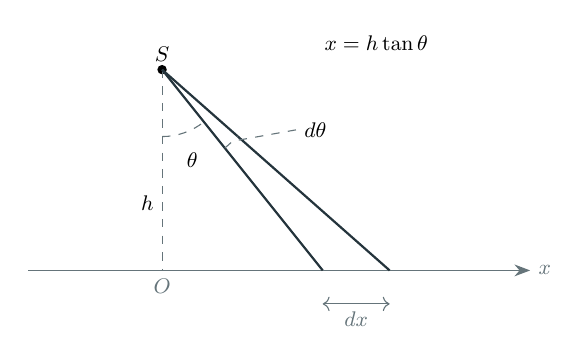
\begin{tikzpicture}[scale=.85,transform shape]

\draw[axis] (-2,0)--(5.5,0) node[right] {$x$};
\coordinate (S) at (0,3);\fill (S) circle (2pt) node[above] {$S$};
\draw[guide] (S)--(0,0) node[below] {$O$};
\draw[object] (S)--(2.4,0);\draw[object] (S)--(3.4,0);
\draw[guide] (0,2) arc[start angle=-90,end angle=-51.34,radius=1];
\node at (.45,1.65) {$\theta$};
\draw[guide] (.937,1.829) arc[start angle=-51.34,end angle=-41.42,radius=1.5];
\node[right] at (2,2.1) {$d\theta$};
\draw[guide] (2,2.1)--(1.05,1.93);
\node[left] at (0,1) {$h$};
\draw[axis,<->] (2.4,-.5)--(3.4,-.5) node[midway,below] {$dx$};
\node at (3.2,3.4) {$x=h\tan\theta$};

\end{tikzpicture}
\figcaption{解图综三.5B\quad 两条相邻射线对应的角度微元与落点微元，密度按雅可比转换。}
\end{minipage}\end{center}
解图综三.5B取向右为$x$正向，从几何关系得到
\[
x=h\tan\theta,\qquad \frac{dx}{d\theta}=h\sec^2\theta
=\frac{h^2+x^2}{h}.
\]
角度密度为常量$c$，其积分$c[\pi/2-(-\pi/2)]=1$给$c=1/\pi$。逆变换$\theta=\arctan(x/h)$在全实轴单调，导数为$h/(h^2+x^2)$。角度密度是$p_\theta=1/\pi$。相邻射线夹成$d\theta$，在直线上截出$dx$；同一事件的概率满足
$p_x(x)\,dx=p_\theta\,d\theta$，故
\[
\boxed{p_x(x)=\frac{h}{\pi(h^2+x^2)}},\quad -\infty<x<\infty.
\]
它的量纲为长度的倒数，它随落点位置改变。远处同样长的线段只对应较小的张角，因而概率密度减小。累积分布和归一化为
\[
F_x(x)=\frac12+\frac1\pi\arctan\frac{x}{h},\qquad
\int_{-\infty}^{\infty}p_x(x)\,dx=1.
\]
\begin{center}\begin{minipage}{.98\linewidth}\centering
\begin{tikzpicture}[scale=.8,transform shape]
\draw[axis] (0,0)--(10.7,0) node[right] {$x/h$};
\draw[axis] (0,0)--(0,3.2) node[above] {$hp_x(x)$};\foreach \y/\lab in {0/0,0.8/.1,1.6/.2,2.4/.3}{\draw[thin] (0,\y)--(-.08,\y) node[left] {$\lab$};}
\node[above] at (5,3.5) {关于零对称的落点密度，远处仍有长尾};
\draw[traj] plot coordinates {(0.000000000,0.149792888) (0.062500000,0.153379256) (0.125000000,0.157093096) (0.187500000,0.160940375) (0.250000000,0.164927402) (0.312500000,0.169060852) (0.375000000,0.173347794) (0.437500000,0.177795712) (0.500000000,0.182412542) (0.562500000,0.187206697) (0.625000000,0.192187101) (0.687500000,0.197363231) (0.750000000,0.202745150) (0.812500000,0.208343554) (0.875000000,0.214169814) (0.937500000,0.220236029) (1.000000000,0.226555079) (1.062500000,0.233140681) (1.125000000,0.240007454) (1.187500000,0.247170987) (1.250000000,0.254647909) (1.312500000,0.262455974) (1.375000000,0.270614143) (1.437500000,0.279142679) (1.500000000,0.288063245) (1.562500000,0.297399018) (1.625000000,0.307174800) (1.687500000,0.317417150) (1.750000000,0.328154522) (1.812500000,0.339417406) (1.875000000,0.351238495) (1.937500000,0.363652851) (2.000000000,0.376698090) (2.062500000,0.390414579) (2.125000000,0.404845642) (2.187500000,0.420037788) (2.250000000,0.436040940) (2.312500000,0.452908686) (2.375000000,0.470698538) (2.437500000,0.489472194) (2.500000000,0.509295818) (2.562500000,0.530240310) (2.625000000,0.552381581) (2.687500000,0.575800812) (2.750000000,0.600584691) (2.812500000,0.626825622) (2.875000000,0.654621874) (2.937500000,0.684077660) (3.000000000,0.715303115) (3.062500000,0.748414134) (3.125000000,0.783532028) (3.187500000,0.820782946) (3.250000000,0.860296990) (3.312500000,0.902206940) (3.375000000,0.946646502) (3.437500000,0.993747937) (3.500000000,1.043638971) (3.562500000,1.096438790) (3.625000000,1.152252982) (3.687500000,1.211167224) (3.750000000,1.273239545) (3.812500000,1.338490980) (3.875000000,1.406894525) (3.937500000,1.478362316) (4.000000000,1.552731152) (4.062500000,1.629746617) (4.125000000,1.709046369) (4.187500000,1.790143472) (4.250000000,1.872411095) (4.312500000,1.955070318) (4.375000000,2.037183272) (4.437500000,2.117654128) (4.500000000,2.195240594) (4.562500000,2.268578253) (4.625000000,2.336219348) (4.687500000,2.396686202) (4.750000000,2.448537586) (4.812500000,2.490444097) (4.875000000,2.521266425) (4.937500000,2.540128768) (5.000000000,2.546479089) (5.062500000,2.540128768) (5.125000000,2.521266425) (5.187500000,2.490444097) (5.250000000,2.448537586) (5.312500000,2.396686202) (5.375000000,2.336219348) (5.437500000,2.268578253) (5.500000000,2.195240594) (5.562500000,2.117654128) (5.625000000,2.037183272) (5.687500000,1.955070318) (5.750000000,1.872411095) (5.812500000,1.790143472) (5.875000000,1.709046369) (5.937500000,1.629746617) (6.000000000,1.552731152) (6.062500000,1.478362316) (6.125000000,1.406894525) (6.187500000,1.338490980) (6.250000000,1.273239545) (6.312500000,1.211167224) (6.375000000,1.152252982) (6.437500000,1.096438790) (6.500000000,1.043638971) (6.562500000,0.993747937) (6.625000000,0.946646502) (6.687500000,0.902206940) (6.750000000,0.860296990) (6.812500000,0.820782946) (6.875000000,0.783532028) (6.937500000,0.748414134) (7.000000000,0.715303115) (7.062500000,0.684077660) (7.125000000,0.654621874) (7.187500000,0.626825622) (7.250000000,0.600584691) (7.312500000,0.575800812) (7.375000000,0.552381581) (7.437500000,0.530240310) (7.500000000,0.509295818) (7.562500000,0.489472194) (7.625000000,0.470698538) (7.687500000,0.452908686) (7.750000000,0.436040940) (7.812500000,0.420037788) (7.875000000,0.404845642) (7.937500000,0.390414579) (8.000000000,0.376698090) (8.062500000,0.363652851) (8.125000000,0.351238495) (8.187500000,0.339417406) (8.250000000,0.328154522) (8.312500000,0.317417150) (8.375000000,0.307174800) (8.437500000,0.297399018) (8.500000000,0.288063245) (8.562500000,0.279142679) (8.625000000,0.270614143) (8.687500000,0.262455974) (8.750000000,0.254647909) (8.812500000,0.247170987) (8.875000000,0.240007454) (8.937500000,0.233140681) (9.000000000,0.226555079) (9.062500000,0.220236029) (9.125000000,0.214169814) (9.187500000,0.208343554) (9.250000000,0.202745150) (9.312500000,0.197363231) (9.375000000,0.192187101) (9.437500000,0.187206697) (9.500000000,0.182412542) (9.562500000,0.177795712) (9.625000000,0.173347794) (9.687500000,0.169060852) (9.750000000,0.164927402) (9.812500000,0.160940375) (9.875000000,0.157093096) (9.937500000,0.153379256) (10.000000000,0.149792888)};
\node[below] at (0,-.12) {$-4$};
\node[below] at (5,-.12) {$0$};
\node[below] at (10,-.12) {$4$};
\end{tikzpicture}
\figcaption{解图综三.5E\quad 关于零对称的落点密度，远处仍有长尾}
\end{minipage}\end{center}
图E把长度用$h$缩放，密度乘$h$后化为标准柯西形状$1/[\pi(1+(x/h)^2)]$。积分的原函数是$\arctan(x/h)/\pi$，两端极限之差为1。尾部$p_x\sim h/(\pi x^2)$，所以$|x|p_x\sim h/(\pi|x|)$产生对数发散，$x^2p_x$趋于正常量而二阶矩发散。关于零的对称性给中位数0和对称主值0；通常期望因两侧一阶积分各自发散而无定义，二阶矩也发散。
\begin{center}\begin{minipage}{.98\linewidth}\centering
\begin{tikzpicture}[scale=.8,transform shape]

\draw[axis] (-2.5,0)--(2.8,0) node[right] {$v_x$};
\draw[axis] (0,-2.4)--(0,2.7) node[above] {$v_y$};
\fill[accent!20,even odd rule] (0,0) circle (1.8) (0,0) circle (1.5);
\draw[object] (0,0) circle (1.5);\draw[object] (0,0) circle (1.8);
\draw[guide] (0,0)--(1.5,0) node[midway,below] {$v$};
\draw[axis,<->] (1.5,.35)--(1.8,.35);
\node[above right] at (1.8,.35) {$dv$};
\node at (5,1) {面积$2\pi v\,dv$};
\node at (5,0) {$f(v)\,dv=F_2\,2\pi v\,dv$};

\end{tikzpicture}
\figcaption{解图综三.5C\quad 等速圆环的面积给二维速率密度，圆环内各方向均须计入。}
\end{minipage}\end{center}
解图综三.5C在速度平面上以$(v_x,v_y)$定位分子。记$\sigma^2=k_{\rm B}T/m$，各分量的归一化密度为
\[
F_1(v_i)=\frac1{\sqrt{2\pi}\sigma}
\exp\left(-\frac{v_i^2}{2\sigma^2}\right).
\]
这里$\sigma$的量纲为速度，归一化因子$1/\sigma$使单分量密度具有速度倒数的量纲。以$v_i/\sigma$代换可把积分化为单位正态积分。独立性给出二维速度密度
\[
F_2(v_x,v_y)=\frac1{2\pi\sigma^2}
\exp\left(-\frac{v_x^2+v_y^2}{2\sigma^2}\right).
\]
联合密度的量纲为速度的负二次方，给的是速度平面小面积的概率。固定速率却未限定方向，所有角度都属于同一事件，故需把小面积元沿角度累加。速率在$v$与$v+dv$间的事件是一条圆环，面积为$2\pi v\,dv$，因此
\[
\boxed{f(v)=\frac{v}{\sigma^2}e^{-v^2/(2\sigma^2)}
=\frac{mv}{k_{\rm B}T}e^{-mv^2/(2k_{\rm B}T)}},\quad v\ge0.
\]
二维圆环面积随$v$成正比，三维球壳面积随$v^2$成正比，各自对应其速度空间的事件。令$u=v^2/(2\sigma^2)$，有$f(v)dv=e^{-u}du$，从而$\int_0^\infty f(v)dv=1$。
\begin{center}\begin{minipage}{.98\linewidth}\centering
\begin{tikzpicture}[scale=.8,transform shape]
\draw[axis] (0,0)--(10.7,0) node[right] {$v/\sigma$};
\draw[axis] (0,0)--(0,3.2) node[above] {$\sigma f(v)$};\foreach \y/\lab in {0/0,0.88/.2,1.76/.4,2.64/.6}{\draw[thin] (0,\y)--(-.08,\y) node[left] {$\lab$};}
\node[above] at (5,3.5) {圆环计数后的二维速率密度，峰在1};
\draw[traj] plot coordinates {(0.000000000,0.000000000) (0.062500000,0.109965630) (0.125000000,0.219725172) (0.187500000,0.329073179) (0.250000000,0.437805491) (0.312500000,0.545719866) (0.375000000,0.652616609) (0.437500000,0.758299188) (0.500000000,0.862574833) (0.562500000,0.965255124) (0.625000000,1.066156558) (0.687500000,1.165101094) (0.750000000,1.261916676) (0.812500000,1.356437726) (0.875000000,1.448505618) (0.937500000,1.537969112) (1.000000000,1.624684770) (1.062500000,1.708517321) (1.125000000,1.789340014) (1.187500000,1.867034916) (1.250000000,1.941493186) (1.312500000,2.012615308) (1.375000000,2.080311288) (1.437500000,2.144500810) (1.500000000,2.205113358) (1.562500000,2.262088297) (1.625000000,2.315374915) (1.687500000,2.364932435) (1.750000000,2.410729978) (1.812500000,2.452746499) (1.875000000,2.490970687) (1.937500000,2.525400821) (2.000000000,2.556044610) (2.062500000,2.582918983) (2.125000000,2.606049860) (2.187500000,2.625471892) (2.250000000,2.641228171) (2.312500000,2.653369918) (2.375000000,2.661956148) (2.437500000,2.667053308) (2.500000000,2.668734903) (2.562500000,2.667081100) (2.625000000,2.662178320) (2.687500000,2.654118813) (2.750000000,2.643000225) (2.812500000,2.628925156) (2.875000000,2.612000710) (2.937500000,2.592338045) (3.000000000,2.570051911) (3.062500000,2.545260201) (3.125000000,2.518083490) (3.187500000,2.488644587) (3.250000000,2.457068089) (3.312500000,2.423479943) (3.375000000,2.388007016) (3.437500000,2.350776671) (3.500000000,2.311916369) (3.562500000,2.271553264) (3.625000000,2.229813829) (3.687500000,2.186823492) (3.750000000,2.142706285) (3.812500000,2.097584513) (3.875000000,2.051578449) (3.937500000,2.004806031) (4.000000000,1.957382595) (4.062500000,1.909420622) (4.125000000,1.861029499) (4.187500000,1.812315313) (4.250000000,1.763380653) (4.312500000,1.714324442) (4.375000000,1.665241785) (4.437500000,1.616223838) (4.500000000,1.567357697) (4.562500000,1.518726307) (4.625000000,1.470408392) (4.687500000,1.422478397) (4.750000000,1.375006457) (4.812500000,1.328058377) (4.875000000,1.281695632) (4.937500000,1.235975379) (5.000000000,1.190950492) (5.062500000,1.146669601) (5.125000000,1.103177149) (5.187500000,1.060513468) (5.250000000,1.018714854) (5.312500000,0.977813662) (5.375000000,0.937838409) (5.437500000,0.898813881) (5.500000000,0.860761257) (5.562500000,0.823698229) (5.625000000,0.787639136) (5.687500000,0.752595104) (5.750000000,0.718574180) (5.812500000,0.685581483) (5.875000000,0.653619350) (5.937500000,0.622687481) (6.000000000,0.592783096) (6.062500000,0.563901079) (6.125000000,0.536034135) (6.187500000,0.509172936) (6.250000000,0.483306270) (6.312500000,0.458421186) (6.375000000,0.434503143) (6.437500000,0.411536145) (6.500000000,0.389502882) (6.562500000,0.368384863) (6.625000000,0.348162547) (6.687500000,0.328815466) (6.750000000,0.310322349) (6.812500000,0.292661236) (6.875000000,0.275809589) (6.937500000,0.259744399) (7.000000000,0.244442287) (7.062500000,0.229879598) (7.125000000,0.216032490) (7.187500000,0.202877022) (7.250000000,0.190389230) (7.312500000,0.178545202) (7.375000000,0.167321145) (7.437500000,0.156693452) (7.500000000,0.146638754) (7.562500000,0.137133981) (7.625000000,0.128156402) (7.687500000,0.119683675) (7.750000000,0.111693882) (7.812500000,0.104165565) (7.875000000,0.097077757) (7.937500000,0.090410006) (8.000000000,0.084142402) (8.062500000,0.078255590) (8.125000000,0.072730790) (8.187500000,0.067549806) (8.250000000,0.062695037) (8.312500000,0.058149483) (8.375000000,0.053896749) (8.437500000,0.049921044) (8.500000000,0.046207183) (8.562500000,0.042740579) (8.625000000,0.039507244) (8.687500000,0.036493779) (8.750000000,0.033687363) (8.812500000,0.031075749) (8.875000000,0.028647249) (8.937500000,0.026390722) (9.000000000,0.024295561) (9.062500000,0.022351683) (9.125000000,0.020549508) (9.187500000,0.018879949) (9.250000000,0.017334394) (9.312500000,0.015904692) (9.375000000,0.014583134) (9.437500000,0.013362439) (9.500000000,0.012235736) (9.562500000,0.011196551) (9.625000000,0.010238785) (9.687500000,0.009356703) (9.750000000,0.008544915) (9.812500000,0.007798362) (9.875000000,0.007112298) (9.937500000,0.006482278) (10.000000000,0.005904142)};
\node[below] at (0,-.12) {$0$};
\node[below] at (2.5,-.12) {$1$};
\node[below] at (5,-.12) {$2$};
\node[below] at (10,-.12) {$4$};
\draw[guide] (2.5,0)--(2.5,2.6687349027355873);
\draw[guide] (3.13328534328875,0)--(3.13328534328875,2.51430828558925);
\draw[guide] (3.5355339059327378,0)--(3.5355339059327378,2.289144418100711);
\node[below] at (3.133285343,-.55) {$\langle v\rangle/\sigma=\sqrt{\pi/2}$};
\node[below] at (3.535533906,-1.05) {$v_{\rm rms}/\sigma=\sqrt2$};
\end{tikzpicture}
\figcaption{解图综三.5D\quad 圆环计数后的二维速率密度，峰在1}
\end{minipage}\end{center}
解图综三.5D画出这个速率曲线。求导
\[
f'(v)=\frac1{\sigma^2}e^{-v^2/(2\sigma^2)}
\left(1-\frac{v^2}{\sigma^2}\right)
\]
可见其唯一最大值在$v=\sigma$。为计算矩，继续使用$u$：
\[
\langle v^q\rangle
=\int_0^\infty(2\sigma^2u)^{q/2}e^{-u}du
=(2\sigma^2)^{q/2}\Gamma(1+q/2),\qquad q>-2.
\]
在原点，矩积分的被积函数按$v^{q+1}$变化，收敛要求$q>-2$；大速率处由高斯指数保证收敛。要计算本题前两阶矩，也可把相关积分联系到三维归一速率密度
\[
f_3(v)=\sqrt{\frac2\pi}\frac{v^2}{\sigma^3}e^{-v^2/(2\sigma^2)},\qquad \int_0^\infty f_3(v)\,\mathrm dv=1.
\]
它由三个独立归一化高斯分量在球壳上积分给出。关系$vf(v)=\sigma\sqrt{\pi/2}\,f_3(v)$直接给二维一阶矩；再乘$v$，用$\int_0^\infty vf_3(v)\mathrm dv=2\sigma\sqrt{2/\pi}$给二阶矩。后一个积分可由$v^2/(2\sigma^2)=u$化为$2\sigma\sqrt{2/\pi}\int_0^\infty ue^{-u}\mathrm du$，分部积分得末积分为1。这样三维归一化与一般伽马矩在同一组积分中给出相同数值。

取$q=1,2$，并用$\Gamma(3/2)=\sqrt\pi/2$、$\Gamma(2)=1$，得到
\[
\boxed{v_{\rm mp}=\sqrt{\frac{k_{\rm B}T}{m}},\quad
\langle v\rangle=\sqrt{\frac{\pi k_{\rm B}T}{2m}},\quad
v_{\rm rms}=\sqrt{\frac{2k_{\rm B}T}{m}}}.
\]
三者按此顺序递增。平均动能$\frac12m\langle v^2\rangle=k_{\rm B}T$，正好等于两个独立平动方向各$k_{\rm B}T/2$之和。
分量法也直接说明二阶矩：$v^2=v_x^2+v_y^2$，两个分量各有方差$\sigma^2$且均值零，所以$\langle v^2\rangle=2\sigma^2$。这一关系与圆环积分和能量均分都一致；一阶速率则把速度矢量的模取平均，按上面的非负速率密度积分，保留方向计数所带来的区别。



\Needspace{13\baselineskip}

\pdfbookmark[2]{第 6 题 四相电源与断线后的浮动星点}{q6}

\section*{第 6 题\quad 四相电源与断线后的浮动星点}\label{q:6}


四相电源的中性点为$N$，各相端点依次为$A,B,C,D$。对$N$的电势为
\[
E_1=E_0\cos\omega t,\quad E_2=E_0\cos(\omega t+\pi/2),\quad
E_3=E_0\cos(\omega t+\pi),\quad E_4=E_0\cos(\omega t+3\pi/2).
\]
四个负载$Z_A,Z_B,Z_C,Z_D$接成星形，星点为$O$。图中$x$是$N$与$O$间的中性线，$y$是$D$相引线；各相电流正方向均由相端流向$O$。

（1）求$U_{AB},U_{AC},U_{AD}$的瞬时表达式。若各相电压有效值为$220\,\mathrm V$，求这三个线电压的峰值。

（2）现同时断开$x,y$，用$Z_A,Z_B,Z_C$和电源电势的复振幅求$A$相电流；须列出所用基尔霍夫方程。

（3）断线情形下取$Z_A=R$、$Z_B=j\omega L$、$Z_C=1/(j\omega C)$，其中$L=R/\omega$、$C=1/(\omega R)$。求$A$相电流的振幅和相位，并求出其余两相电流和各相平均功率。负载与电源均为理想元件，采用$\Re(\widetilde E e^{j\omega t})$约定。


\begin{center}\begin{minipage}{.98\linewidth}\centering
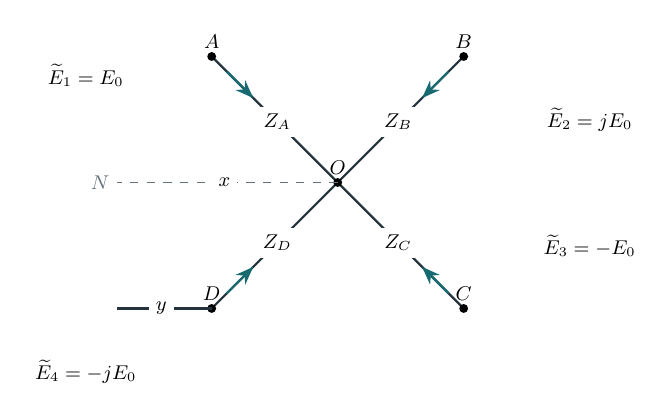
\begin{tikzpicture}[scale=.8,transform shape]

\coordinate (A) at (-2,2);\coordinate (B) at (2,2);
\coordinate (C) at (2,-2);\coordinate (D) at (-2,-2);
\coordinate (O) at (0,0);
\foreach \p/\z in {A/A,B/B,C/C,D/D}{
\draw[object] (\p)--(O);
\node[fill=white,inner sep=3pt] at ($(\p)!.52!(O)$) {$Z_\z$};
\fill (\p) circle (2pt) node[above] {$\p$};
}
\fill (O) circle (2pt) node[above] {$O$};
\foreach \p in {A,B,C,D}{\draw[motion] ($(\p)!.12!(O)$)--($(\p)!.33!(O)$);}

\draw[guide] (0,0)--(-3.5,0) node[left] {$N$};
\node[fill=white] at (-1.8,0) {$x$};
\draw[object] (-2,-2)--(-3.5,-2);
\node[fill=white] at (-2.8,-2) {$y$};
\node at (4,1) {$\widetilde E_2=jE_0$};
\node at (4,-1) {$\widetilde E_3=-E_0$};
\node at (-4,1.7) {$\widetilde E_1=E_0$};
\node at (-4,-3) {$\widetilde E_4=-jE_0$};

\end{tikzpicture}
\figcaption{图综三.6\quad 四相星形负载；$x$为中性线，$y$为$D$相引线。}
\end{minipage}\end{center}

\Needspace{6\baselineskip}\subsection*{解答}


图综三.6中的相序以相邻电势超前$\pi/2$规定。用峰值复振幅表示，四相依次为
\[
(\widetilde E_1,\widetilde E_2,\widetilde E_3,\widetilde E_4)
=E_0(1,j,-1,-j).
\]
这里$\widetilde E_k$只含振幅和初相，瞬时实电势由$E_k(t)=\Re(\widetilde E_ke^{j\omega t})$恢复。后面的电流和星点电势采用相同约定。
\begin{center}\begin{minipage}{.98\linewidth}\centering
\begin{tikzpicture}[scale=.8,transform shape]
\draw[axis] (-3,0)--(3,0) node[right] {实轴};\draw[axis] (0,-2.7)--(0,2.8) node[above] {虚轴};
\draw[motion] (0,0)--(2,0) node[above right] {$\widetilde E_1$};\draw[motion] (0,0)--(0,2) node[above left] {$\widetilde E_2$};\draw[motion] (0,0)--(-2,0) node[above left] {$\widetilde E_3$};\draw[motion] (0,0)--(0,-2) node[below left] {$\widetilde E_4$};
\draw[force] (0,2)--(2,0) node[midway,above right] {$\widetilde U_{AB}$};\draw[force,color=warm] (0,-2)--(2,0) node[midway,below right] {$\widetilde U_{AD}$};
\draw[guide] (-2,0)--(-2,-.45);\draw[guide] (2,0)--(2,-.45);\draw[force] (-2,-.4)--(2,-.4) node[midway,below,fill=white] {$\widetilde U_{AC}=2E_0$};
\node at (0,-3.25) {$|\widetilde U_{AB}|=|\widetilde U_{AD}|=\sqrt2E_0$};
\end{tikzpicture}
\figcaption{解图综三.6A\quad 相量差箭头从被减相量端点指向另一端点}
\end{minipage}\end{center}
解图综三.6A的线电压是两个相端对同一参考点$N$的电势之差。$B$端的$+jE_0$从$A$端电势中减去，给第四象限；$D$端的$-jE_0$被减去，给第一象限；$C$与$A$相反，差矢量沿正实轴。因此
\[
\widetilde U_{AB}=(1-j)E_0=\sqrt2E_0e^{-j\pi/4},\quad
\widetilde U_{AC}=2E_0,\quad
\widetilde U_{AD}=(1+j)E_0=\sqrt2E_0e^{j\pi/4}.
\]
乘回公共因子$e^{j\omega t}$再取实部，返回时间域：
\[
\boxed{U_{AB}=\sqrt2E_0\cos(\omega t-\pi/4)},\quad
\boxed{U_{AC}=2E_0\cos\omega t},\quad
\boxed{U_{AD}=\sqrt2E_0\cos(\omega t+\pi/4)}.
\]
各相有效值$220\,\mathrm V$对应$E_0=220\sqrt2\,\mathrm V$，所以三个线电压的峰值分别为
\[
\boxed{440\,\mathrm V,\quad440\sqrt2\,\mathrm V\approx622\,\mathrm V,\quad440\,\mathrm V}.
\]
相邻相差$\pi/2$，线电压峰值为$\sqrt2E_0$；相反相差$\pi$，线电压峰值为$2E_0$。
\begin{center}\begin{minipage}{.98\linewidth}\centering
\begin{tikzpicture}[scale=.8,transform shape]
\draw[object] (0,4)--(6,4) node[right] {$N:\ 0$};\draw[object] (0,0)--(6,0) node[right] {$O:\ \widetilde V$};
\foreach \x/\e/\z in {0/1/A,3/2/B,6/3/C}{\draw[object] (\x,4)--(\x,0);\node[draw,circle,fill=white,minimum size=10mm] at (\x,3) {$\widetilde E_\e$};\node[fill=white] at (\x,3.62) {$-$};\node[fill=white] at (\x,2.4) {$+$};\node[draw,fill=white,minimum width=11mm,minimum height=8mm] at (\x,1.5) {$Z_\z$};\draw[motion] (\x,.95)--(\x,.25) node[midway,right] {$\widetilde I_\z$};}
\node[align=left] at (8.6,2.3) {中性线开路\\$D$相开路，$I_D=0$};\node at (3,-.8) {$I_A+I_B+I_C=0$};
\end{tikzpicture}
\figcaption{解图综三.6B\quad 各电源下端为正端，三负载汇于浮动星点；参考轨$N$与星点$O$分别画出}
\end{minipage}\end{center}
解图综三.6B保留断线后仍相互构成回路的三条支路。$Z_D$的一端悬空，故$I_D=0$；$O$的电势由其余三条支路共同决定。以$N$为电势零点，记星点的复电势为$\widetilde V$，各负载从相端向$O$的电压降为$\widetilde E_k-\widetilde V$，所以
\[
\widetilde I_A=\frac{\widetilde E_1-\widetilde V}{Z_A},\quad
\widetilde I_B=\frac{\widetilde E_2-\widetilde V}{Z_B},\quad
\widetilde I_C=\frac{\widetilde E_3-\widetilde V}{Z_C}.
\]
在浮动节点$O$应用电流定律，并沿$A\to O\to B$、$A\to O\to C$两路径应用电压定律：
\[
\widetilde I_A+\widetilde I_B+\widetilde I_C=0,
\]
\[
Z_A\widetilde I_A-Z_B\widetilde I_B=\widetilde U_{AB},\qquad
Z_A\widetilde I_A-Z_C\widetilde I_C=\widetilde U_{AC}.
\]
这两个电压式中的负号，来自沿$O\to B$或$O\to C$行走时与相应电流的正方向相反。先解出另外两支路，保留分式消元的中间步骤：
\[
\widetilde I_B=\frac{Z_A}{Z_B}\widetilde I_A-\frac{\widetilde U_{AB}}{Z_B},\quad
\widetilde I_C=\frac{Z_A}{Z_C}\widetilde I_A-\frac{\widetilde U_{AC}}{Z_C},
\]
\[
\widetilde I_A\left(1+\frac{Z_A}{Z_B}+\frac{Z_A}{Z_C}\right)
=\frac{\widetilde U_{AB}}{Z_B}+\frac{\widetilde U_{AC}}{Z_C}.
\]
乘以$Z_BZ_C$，得到
\[
\widetilde I_A(Z_AZ_B+Z_BZ_C+Z_CZ_A)
=Z_C\widetilde U_{AB}+Z_B\widetilde U_{AC}.
\]
因此在分母不为零时
\[
\boxed{\widetilde I_A=
\frac{Z_C\widetilde U_{AB}+Z_B\widetilde U_{AC}}
{Z_AZ_B+Z_BZ_C+Z_CZ_A}
=\frac{[(1-j)Z_C+2Z_B]E_0}
{Z_AZ_B+Z_BZ_C+Z_CZ_A}}.
\]
其中$(1-j)=\sqrt2e^{-j\pi/4}$，把这一形式与时间因子相乘，即为复电流$\widetilde I_Ae^{j\omega t}$。节点形式也可直接由三条支路电流和为零整理出来：
\[
\widetilde V=
\frac{\widetilde E_1/Z_A+\widetilde E_2/Z_B+\widetilde E_3/Z_C}
{1/Z_A+1/Z_B+1/Z_C}.
\]
它把每相电势按该支路导纳加权，再除以总导纳；代入$A$支路所得电流与上面的消元结果相同。消元式中的阻抗组合$D=Z_AZ_B+Z_BZ_C+Z_CZ_A$非零时，方程给唯一稳态复振幅；$D=0$的理想无耗散情形，要由回路方程的相容性与初始储能共同确定响应。本题指定的电阻使$D=R^2>0$。

现在代入$Z_A=R,Z_B=jR,Z_C=-jR$。分母的两项纯虚贡献相反，$Z_BZ_C=R^2$留下实项：
\[
Z_AZ_B+Z_BZ_C+Z_CZ_A=R^2,
\]
分子中的阻抗组合为
\[
(1-j)Z_C+2Z_B=(1-j)(-jR)+2jR=(-1+j)R.
\]
复数$(-1+j)R$位于第二象限，其模为$\sqrt2R$，辐角为$3\pi/4$，故
\[
\boxed{\widetilde I_A=(-1+j)\frac{E_0}{R}
=\frac{\sqrt2E_0}{R}e^{j3\pi/4}},\qquad
\boxed{I_A(t)=\frac{\sqrt2E_0}{R}\cos(\omega t+3\pi/4)}.
\]
$A$相电流比$E_1$超前$3\pi/4$。电阻的实际两端电压是$E_1-V$，其相量$R\widetilde I_A=(-1+j)E_0$与电流同相；$E_1$则是相端对$N$的电势。

为求另外两电流，先在节点式中逐项代入。导纳和$1/R+1/(jR)+1/(-jR)=1/R$，而分子是$E_0/R+jE_0/(jR)-E_0/(-jR)=(2-j)E_0/R$，从而得到星点。随后用$\widetilde I_B=(jE_0-\widetilde V)/(jR)$及$\widetilde I_C=(-E_0-\widetilde V)/(-jR)$，得
\[
\widetilde V=(2-j)E_0,\quad
\widetilde I_B=(2+2j)\frac{E_0}{R},\quad
\widetilde I_C=(-1-3j)\frac{E_0}{R}.
\]
\begin{center}\begin{minipage}{.98\linewidth}\centering
\begin{tikzpicture}[scale=.8,transform shape]
\draw[axis] (-2,0)--(3,0) node[right] {实部};\draw[axis] (0,-3.7)--(0,3.7) node[above] {虚部};
\draw[motion] (0,0)--(-1,1) node[above left] {$\widetilde I_A$};\draw[motion] (0,0)--(2,2) node[above right] {$\widetilde I_B$};\draw[motion] (0,0)--(-1,-3) node[below left] {$\widetilde I_C$};
\draw[guide,->] (-1,1)--(1,3);\draw[guide,->] (1,3)--(0,0);\node[align=left] at (5.5,1) {单位$E_0/R$\\$(-1+j)+(2+2j)+(-1-3j)=0$};
\end{tikzpicture}
\figcaption{解图综三.6C\quad 共起点电流相量与首尾相接的闭三角形采用相同尺度}
\end{minipage}\end{center}
解图综三.6C中三个相量首尾相接回到起点：相加得$(-1+j)+(2+2j)+(-1-3j)=0$，三个相量的实部和、虚部和分别为零，恢复到时间域后的三电流总和恒为零，浮动节点每一瞬间都满足电流守恒。
\begin{center}\begin{minipage}{.98\linewidth}\centering
\begin{tikzpicture}[scale=.8,transform shape]
\draw[axis] (0,0)--(10.7,0) node[right] {$\omega t$};
\draw[axis] (0,0)--(0,3.2) node[above] {归一化瞬时值};\foreach \y/\lab in {0.8/-1,2.4/1}{\draw[thin] (0,\y)--(-.08,\y) node[left] {$\lab$};}
\node[above] at (5,3.5) {虚线$E_1/E_0$，实线$RI_A/E_0=(E_1-V)/E_0$};
\draw[guide] plot coordinates {(0.000000000,2.400000000) (0.055555556,2.399512662) (0.111111111,2.398051240) (0.166666667,2.395617516) (0.222222222,2.392214455) (0.277777778,2.387846202) (0.333333333,2.382518081) (0.388888889,2.376236581) (0.444444444,2.369009357) (0.500000000,2.360845213) (0.555555556,2.351754097) (0.611111111,2.341747084) (0.666666667,2.330836366) (0.722222222,2.319035237) (0.777777778,2.306358074) (0.833333333,2.292820323) (0.888888889,2.278438477) (0.944444444,2.263230058) (1.000000000,2.247213595) (1.055555556,2.230408603) (1.111111111,2.212835554) (1.166666667,2.194515860) (1.222222222,2.175471840) (1.277777778,2.155726696) (1.333333333,2.135304485) (1.388888889,2.114230088) (1.444444444,2.092529180) (1.500000000,2.070228202) (1.555555556,2.047354323) (1.611111111,2.023935411) (1.666666667,2.000000000) (1.722222222,1.975577250) (1.777777778,1.950696917) (1.833333333,1.925389314) (1.888888889,1.899685275) (1.944444444,1.873616115) (2.000000000,1.847213595) (2.055555556,1.820509885) (2.111111111,1.793537516) (2.166666667,1.766329353) (2.222222222,1.738918542) (2.277777778,1.711338481) (2.333333333,1.683622771) (2.388888889,1.655805179) (2.444444444,1.627919597) (2.500000000,1.600000000) (2.555555556,1.572080403) (2.611111111,1.544194821) (2.666666667,1.516377229) (2.722222222,1.488661519) (2.777777778,1.461081458) (2.833333333,1.433670647) (2.888888889,1.406462484) (2.944444444,1.379490115) (3.000000000,1.352786405) (3.055555556,1.326383885) (3.111111111,1.300314725) (3.166666667,1.274610686) (3.222222222,1.249303083) (3.277777778,1.224422750) (3.333333333,1.200000000) (3.388888889,1.176064589) (3.444444444,1.152645677) (3.500000000,1.129771798) (3.555555556,1.107470820) (3.611111111,1.085769912) (3.666666667,1.064695515) (3.722222222,1.044273304) (3.777777778,1.024528160) (3.833333333,1.005484140) (3.888888889,0.987164446) (3.944444444,0.969591397) (4.000000000,0.952786405) (4.055555556,0.936769942) (4.111111111,0.921561523) (4.166666667,0.907179677) (4.222222222,0.893641926) (4.277777778,0.880964763) (4.333333333,0.869163634) (4.388888889,0.858252916) (4.444444444,0.848245903) (4.500000000,0.839154787) (4.555555556,0.830990643) (4.611111111,0.823763419) (4.666666667,0.817481919) (4.722222222,0.812153798) (4.777777778,0.807785545) (4.833333333,0.804382484) (4.888888889,0.801948760) (4.944444444,0.800487338) (5.000000000,0.800000000) (5.055555556,0.800487338) (5.111111111,0.801948760) (5.166666667,0.804382484) (5.222222222,0.807785545) (5.277777778,0.812153798) (5.333333333,0.817481919) (5.388888889,0.823763419) (5.444444444,0.830990643) (5.500000000,0.839154787) (5.555555556,0.848245903) (5.611111111,0.858252916) (5.666666667,0.869163634) (5.722222222,0.880964763) (5.777777778,0.893641926) (5.833333333,0.907179677) (5.888888889,0.921561523) (5.944444444,0.936769942) (6.000000000,0.952786405) (6.055555556,0.969591397) (6.111111111,0.987164446) (6.166666667,1.005484140) (6.222222222,1.024528160) (6.277777778,1.044273304) (6.333333333,1.064695515) (6.388888889,1.085769912) (6.444444444,1.107470820) (6.500000000,1.129771798) (6.555555556,1.152645677) (6.611111111,1.176064589) (6.666666667,1.200000000) (6.722222222,1.224422750) (6.777777778,1.249303083) (6.833333333,1.274610686) (6.888888889,1.300314725) (6.944444444,1.326383885) (7.000000000,1.352786405) (7.055555556,1.379490115) (7.111111111,1.406462484) (7.166666667,1.433670647) (7.222222222,1.461081458) (7.277777778,1.488661519) (7.333333333,1.516377229) (7.388888889,1.544194821) (7.444444444,1.572080403) (7.500000000,1.600000000) (7.555555556,1.627919597) (7.611111111,1.655805179) (7.666666667,1.683622771) (7.722222222,1.711338481) (7.777777778,1.738918542) (7.833333333,1.766329353) (7.888888889,1.793537516) (7.944444444,1.820509885) (8.000000000,1.847213595) (8.055555556,1.873616115) (8.111111111,1.899685275) (8.166666667,1.925389314) (8.222222222,1.950696917) (8.277777778,1.975577250) (8.333333333,2.000000000) (8.388888889,2.023935411) (8.444444444,2.047354323) (8.500000000,2.070228202) (8.555555556,2.092529180) (8.611111111,2.114230088) (8.666666667,2.135304485) (8.722222222,2.155726696) (8.777777778,2.175471840) (8.833333333,2.194515860) (8.888888889,2.212835554) (8.944444444,2.230408603) (9.000000000,2.247213595) (9.055555556,2.263230058) (9.111111111,2.278438477) (9.166666667,2.292820323) (9.222222222,2.306358074) (9.277777778,2.319035237) (9.333333333,2.330836366) (9.388888889,2.341747084) (9.444444444,2.351754097) (9.500000000,2.360845213) (9.555555556,2.369009357) (9.611111111,2.376236581) (9.666666667,2.382518081) (9.722222222,2.387846202) (9.777777778,2.392214455) (9.833333333,2.395617516) (9.888888889,2.398051240) (9.944444444,2.399512662) (10.000000000,2.400000000)};
\draw[traj] plot coordinates {(0.000000000,0.800000000) (0.055555556,0.772567741) (0.111111111,0.746143581) (0.166666667,0.720759713) (0.222222222,0.696447064) (0.277777778,0.673235255) (0.333333333,0.651152567) (0.388888889,0.630225902) (0.444444444,0.610480759) (0.500000000,0.591941191) (0.555555556,0.574629789) (0.611111111,0.558567642) (0.666666667,0.543774319) (0.722222222,0.530267846) (0.777777778,0.518064675) (0.833333333,0.507179677) (0.888888889,0.497626112) (0.944444444,0.489415619) (1.000000000,0.482558203) (1.055555556,0.477062217) (1.111111111,0.472934358) (1.166666667,0.470179655) (1.222222222,0.468801463) (1.277777778,0.468801463) (1.333333333,0.470179655) (1.388888889,0.472934358) (1.444444444,0.477062217) (1.500000000,0.482558203) (1.555555556,0.489415619) (1.611111111,0.497626112) (1.666666667,0.507179677) (1.722222222,0.518064675) (1.777777778,0.530267846) (1.833333333,0.543774319) (1.888888889,0.558567642) (1.944444444,0.574629789) (2.000000000,0.591941191) (2.055555556,0.610480759) (2.111111111,0.630225902) (2.166666667,0.651152567) (2.222222222,0.673235255) (2.277777778,0.696447064) (2.333333333,0.720759713) (2.388888889,0.746143581) (2.444444444,0.772567741) (2.500000000,0.800000000) (2.555555556,0.828406936) (2.611111111,0.857753939) (2.666666667,0.888005254) (2.722222222,0.919124026) (2.777777778,0.951072340) (2.833333333,0.983811272) (2.888888889,1.017300935) (2.944444444,1.051500528) (3.000000000,1.086368382) (3.055555556,1.121862018) (3.111111111,1.157938191) (3.166666667,1.194552948) (3.222222222,1.231661680) (3.277777778,1.269219176) (3.333333333,1.307179677) (3.388888889,1.345496934) (3.444444444,1.384124265) (3.500000000,1.423014606) (3.555555556,1.462120577) (3.611111111,1.501394533) (3.666666667,1.540788625) (3.722222222,1.580254856) (3.777777778,1.619745144) (3.833333333,1.659211375) (3.888888889,1.698605467) (3.944444444,1.737879423) (4.000000000,1.776985394) (4.055555556,1.815875735) (4.111111111,1.854503066) (4.166666667,1.892820323) (4.222222222,1.930780824) (4.277777778,1.968338320) (4.333333333,2.005447052) (4.388888889,2.042061809) (4.444444444,2.078137982) (4.500000000,2.113631618) (4.555555556,2.148499472) (4.611111111,2.182699065) (4.666666667,2.216188728) (4.722222222,2.248927660) (4.777777778,2.280875974) (4.833333333,2.311994746) (4.888888889,2.342246061) (4.944444444,2.371593064) (5.000000000,2.400000000) (5.055555556,2.427432259) (5.111111111,2.453856419) (5.166666667,2.479240287) (5.222222222,2.503552936) (5.277777778,2.526764745) (5.333333333,2.548847433) (5.388888889,2.569774098) (5.444444444,2.589519241) (5.500000000,2.608058809) (5.555555556,2.625370211) (5.611111111,2.641432358) (5.666666667,2.656225681) (5.722222222,2.669732154) (5.777777778,2.681935325) (5.833333333,2.692820323) (5.888888889,2.702373888) (5.944444444,2.710584381) (6.000000000,2.717441797) (6.055555556,2.722937783) (6.111111111,2.727065642) (6.166666667,2.729820345) (6.222222222,2.731198537) (6.277777778,2.731198537) (6.333333333,2.729820345) (6.388888889,2.727065642) (6.444444444,2.722937783) (6.500000000,2.717441797) (6.555555556,2.710584381) (6.611111111,2.702373888) (6.666666667,2.692820323) (6.722222222,2.681935325) (6.777777778,2.669732154) (6.833333333,2.656225681) (6.888888889,2.641432358) (6.944444444,2.625370211) (7.000000000,2.608058809) (7.055555556,2.589519241) (7.111111111,2.569774098) (7.166666667,2.548847433) (7.222222222,2.526764745) (7.277777778,2.503552936) (7.333333333,2.479240287) (7.388888889,2.453856419) (7.444444444,2.427432259) (7.500000000,2.400000000) (7.555555556,2.371593064) (7.611111111,2.342246061) (7.666666667,2.311994746) (7.722222222,2.280875974) (7.777777778,2.248927660) (7.833333333,2.216188728) (7.888888889,2.182699065) (7.944444444,2.148499472) (8.000000000,2.113631618) (8.055555556,2.078137982) (8.111111111,2.042061809) (8.166666667,2.005447052) (8.222222222,1.968338320) (8.277777778,1.930780824) (8.333333333,1.892820323) (8.388888889,1.854503066) (8.444444444,1.815875735) (8.500000000,1.776985394) (8.555555556,1.737879423) (8.611111111,1.698605467) (8.666666667,1.659211375) (8.722222222,1.619745144) (8.777777778,1.580254856) (8.833333333,1.540788625) (8.888888889,1.501394533) (8.944444444,1.462120577) (9.000000000,1.423014606) (9.055555556,1.384124265) (9.111111111,1.345496934) (9.166666667,1.307179677) (9.222222222,1.269219176) (9.277777778,1.231661680) (9.333333333,1.194552948) (9.388888889,1.157938191) (9.444444444,1.121862018) (9.500000000,1.086368382) (9.555555556,1.051500528) (9.611111111,1.017300935) (9.666666667,0.983811272) (9.722222222,0.951072340) (9.777777778,0.919124026) (9.833333333,0.888005254) (9.888888889,0.857753939) (9.944444444,0.828406936) (10.000000000,0.800000000)};
\node[below] at (0,-.12) {$0$};
\node[below] at (5,-.12) {$\pi$};
\node[below] at (10,-.12) {$2\pi$};
\draw[guide] (0,1.6)--(10,1.6);\node[left] at (0,1.6) {$0$};
\end{tikzpicture}
\figcaption{解图综三.6D\quad 虚线$E_1/E_0$，实线$RI_A/E_0=(E_1-V)/E_0$}
\end{minipage}\end{center}
解图综三.6D用$E_0$归一化相端电势、用$E_0/R$归一化电阻电流；实线也是实际电阻电压$(E_1-V)/E_0$，所以电流与其两端电压在整个周期逐点同相。电阻平均发热由正弦电流平方取平均：
\[
\boxed{\overline P_R=\frac R2|\widetilde I_A|^2=\frac{E_0^2}{R}}.
\]
这里$I_A$的峰值为$\sqrt2E_0/R$，峰值平方乘$1/2$给电流平方的周期平均，与式中的峰值相量约定对应。电感、电容在稳态经过完整周期恢复相同储能，各自平均有功为零。

按电流从电源流向负载为供能正方向，各相电源的平均输出为
\[
\overline P_k=\frac12\Re(\widetilde E_k\widetilde I_k^*),\qquad
(\overline P_A,\overline P_B,\overline P_C)
=\left(-\frac12,1,\frac12\right)\frac{E_0^2}{R}.
\]
例如$\widetilde E_1\widetilde I_A^*/2=(-1-j)E_0^2/(2R)$，实部为负；$B$相乘积为$(1+j)E_0^2/R$，$C$相为$(1-3j)E_0^2/(2R)$。三项实部相加为$E_0^2/R$，恰好等于电阻耗散。$A$相电源平均吸收能量，$B,C$相共同供能；电容、电感平均储能变化为零。浮动星点相对$N$的电压幅值为$\sqrt5E_0$；电阻两端幅值则为$\sqrt2E_0$，二者对应图B中不同的两个端点。



\end{document}
